%%% The main file. It contains definitions of basic parameters and includes all other parts.

%% Settings for single-side (simplex) printing
% Margins: left 40mm, right 25mm, top and bottom 25mm
% (but beware, LaTeX adds 1in implicitly)
\documentclass[12pt,notitlepage,a4paper,openright]{report}
\pagestyle{plain}

\PassOptionsToPackage{hyperfootnotes=false}{hyperref}

% fix pdfx
\usepackage{etoolbox}
% \makeatletter
% \@ifl@t@r\fmtversion{2021-06-01}%
%  {\AddToHook{package/after/xmpincl}
%    {\patchcmd\mcs@xmpincl@patchFile{\if\par}{\ifx\par}{}{\fail}}}{}
% \makeatother

\usepackage[usenames,dvipsnames,svgnames,table,rgb]{xcolor}
\usepackage[a-2u]{pdfx}
\usepackage{fontspec}
\usepackage[czech,english]{babel}
\usepackage{lmodern}
\usepackage{textcomp}
\usepackage{bbm}
\usepackage[defaultlines=4,all]{nowidow}

% Turn this on when needed:
%\usepackage{microtype}

\usepackage{graphicx}
\usepackage[twoside, inner=3.7cm, outer=2.9cm, top=2.6cm, bottom=3.4cm]{geometry}
\usepackage{thesis}
\usepackage[round]{natbib}
\usepackage{multirow}
\usepackage{arydshln} % dashed lines in tables
\usepackage{array}
\usepackage{amssymb,latexsym,pifont}
\usepackage{amsmath}
\usepackage{latexsym}
\usepackage{enumitem} % custom lists
\usepackage[normalem]{ulem} % underlining
\usepackage{setspace} % line spacing
\usepackage{varioref} % nice references (above/below)
\usepackage[above,section]{placeins} % avoid figures pushed at end of chapters
\usepackage{listings}

\usepackage{pifont}% http://ctan.org/pkg/pifont
\usepackage{tabularx}
\usepackage{booktabs} % nicer lines in table
\usepackage{multicol}
\usepackage{tikz}
\usepackage{pgfplots}
\pgfplotsset{compat=1.18}
\usepackage{gnuplot-lua-tikz}
\usetikzlibrary{shapes.geometric}
\usepackage{epstopdf}
\usepackage{algorithmicx}
\usepackage{algorithm}
\usepackage{algpseudocode}
\usepackage{mathtools}
\usepackage{relsize}
\usepackage{subfig}
\captionsetup[subfigure]{justification=raggedright}

% acronyms and glossaries
\usepackage[acronym, nomain]{glossaries}
\usepackage[shortcuts=ac]{glossaries-extra}
\makeglossaries
\preto\chapter{\glsresetall}

\setabbreviationstyle[acronym]{long-short}

% \usepackage{subcaption} % sub figures in a fiture
\usepackage{standalone} % include standoalone tikz images
\usepackage{bibentry}

\usepackage{inconsolata}

\usepackage{multirow}
\usepackage{tablefootnote}
\usepackage{float}


\usepackage{pifont}% http://ctan.org/pkg/pifont
\usepackage{color, colortbl}

\definecolor{tablegray}{rgb}{0.9,0.9,0.9}
\definecolor{darkgreen}{rgb}{0,0.5,0}
\definecolor{lightblue}{rgb}{0.7,0.9,1}
\definecolor{lblue}{rgb}{0.25,0.5,1}

\usepackage[normalem]{ulem}

% hack bibentry command for list of publications
\makeatletter
\renewcommand\bibentry[1]{\nocite{#1}{\frenchspacing
     \@nameuse{BR@r@#1\@extra@b@citeb}}}
\makeatother

\hypersetup{
    colorlinks=false,
    pdfborder={0 0 0},
    unicode=true,
}

\input{acronyms}

% Czech babel conflicts with cline, hacky fix (http://tex.stackexchange.com/questions/111999/slovak-and-czech-babel-gives-problems-with-cmidrule-and-cline):
% - basically disables hyphenation in tables, but it's not used anyway so it doesn't matter
\preto\tabular{\shorthandoff{-}}
\preto\tikzpicture{\shorthandoff{-}}
%
%
\hyphenation{%
da-ta-sets
da-ta-set
} % -- custom hyphenation

% \setmainfont[Ligatures=Common]{Linux Libertine}
\setsansfont[Scale=MatchLowercase]{DejaVu Sans}
\setmonofont[Scale=MatchLowercase]{DejaVu Sans Mono}


\setstretch{1.1} % line spacing

\expandafter\def\expandafter\quote\expandafter{\quote\small} % smaller quotations font

% orphan & widow control
%\clubpenalty 10000
%\widowpenalty 10000

% gaps between text and footnotes
\def\footnoteskip#1{
  \renewcommand\footnoterule{
     \vspace{#1}
     \hrule width 0.4\columnwidth%
     \vspace{3pt}
}
}
\footnoteskip{0.8em}


\setcounter{tocdepth}{2}
\setcounter{secnumdepth}{2}

%% cutting down warnings
%\hfuzz=2pt
%\hbadness=10000

% force-ordering citations according to dummy keys
\newcommand{\dummybiborderkey}[1]{}

\input{macros}

\newcommand{\veryshortarrow}[1][3pt]{\mathrel{%
     \vcenter{\hbox{\rule[-.5\fontdimen8\textfont3]{#1}{\fontdimen8\textfont3}}}%
     \mkern-4mu\hbox{\usefont{U}{lasy}{m}{n}\symbol{41}}}}
\newcommand{\pz}{\phantom{0}}
\newcommand{\paperdisclaim}[1]{%
\begin{center}\begin{minipage}{0.9\textwidth}
\footnotesize\it #1
\end{minipage}\end{center}
}

\def\ignorecolumn#1\unskip{}

\definecolor{lightblue}{rgb}{0.6,0.8,1.0}
\definecolor{pastelgreen}{rgb}{0.65,0.8,0.4}
\definecolor{pastelyellow}{rgb}{1.0,0.8,0.5}


\title{Doctoral Thesis Template}

\def\fulldate{}
\author{Random Author}
\date{2022}
\dept{Institute of Formal and Applied Linguistics}
\supervisor{Ondra}
\studyprogram{Computer Science}
\studyfield{Computational Linguistics}


\begin{document}

%
%
%
\renewcommand{\thepage}{\roman{page}}
\selectlanguage{english}
\maketitle

\pagestyle{plain}
\normalsize
\setcounter{page}{2}

\cleardoublepage{}
\ \vspace{10mm}

\noindent \it

\vspace{\fill}
\noindent \rm
I declare that I carried out this doctoral thesis independently,
  and only with the cited sources, literature and other professional sources.

I understand that my work relates to the rights and obligations
  under the Act No.~121/2000 Coll., the Copyright Act, as amended,
  in particular the fact that Charles University has the right
  to conclude a license agreement on the use of this work as a school work
  pursuant to Section~60 paragraph~1 of the Copyright Act.

\vspace{2cm}
\noindent Prague, November 17, 1989 (TODO) \hspace{\fill}\theauthor % doplňte patřičné
                                                             % datum, jméno a
                                                             % příjmení

%%%   Do not forget to SIGN the printed book here!
%%%                  *********

\definecolor{darkgreen}{rgb}{0,0.5,0}
\definecolor{lightblue}{rgb}{0.7,0.9,1}
\definecolor{lblue}{rgb}{0.25,0.5,1}
\newcommand{\rewrite}[1] {
  {\color{blue}\textbf{TO BE REWRITTEN:} #1}
  }
\newcommand{\todo}[1] {
  {\color{red}\textbf{TODO:} #1}
  }
\newcommand{\VH}[1] {
  {\color{darkgreen}\emph{VH:} #1}
  }

\cleardoublepage{} % new page
\pagestyle{plain}

\addcontentsline{toc}{chapter}{English Abstract}

%\selectlanguage{english}
\begin{description}[leftmargin=7.5em,labelwidth=7em,labelindent=0em,labelsep=0.5em]
\item[Title:] \thetitle{}
\item[Author:] \theauthor{}
\item[Department:] \thedept{}
\item[Supervisor:] \thesupervisor{},\\ \thedept{}
\end{description}
\subsubsection{Abstract:}

This thesis focuses on developing and improving task-oriented dialogue systems design in the rapidly growing landscape of artificial intelligence and natural language processing.
We propose techniques that can substantially decrease development and deployment costs, motivated by the desire to make these systems more adaptable and scalable.
We introduce multiple approaches to achieving these goals, some of which we pioneer.

Firstly, we present a weakly supervised automatic data annotation pipeline that can transform raw data into a refined set of semantically coherent concepts, bypassing the need for exhaustive manual annotations and significantly streamlining the development process.

We also explore the largely uninvestigated field of latent variable models in task-oriented dialogue system modeling.
These models offer excellent capabilities with the potential to uncover the structure of behavioral patterns seen in the dialogue through inspection of the latent space and comparison with actions taken by the model.

Moreover, we harness the power of large pre-trained language models using in-context learning, following progress in the field.
Our proposed retrieval-augmented method performs well with merely a few training examples.
It shows great promise regarding human evaluation, implying a substantial leap in efficiently using computational resources to train conversational AI.
This brings us closer to more flexible and general-purpose systems.

In summary, the research presented in this thesis brings exciting innovations, uncovering new pathways in developing task-oriented dialogue systems.
It moves towards a future where dialogue systems can adapt, learn, and interact efficiently, potentially transforming how people interact with technology.

\begin{description}[leftmargin=7.5em,labelwidth=7em,labelindent=0em,labelsep=0.5em]
        %
\item[Keywords:]dialogue systems, semi-supervised learning, language models, variational training, hierarchical models, clustering
    %
\end{description}


\cleardoublepage{}
\addcontentsline{toc}{chapter}{Czech Abstract}
\selectlanguage{czech}
\begin{description}[leftmargin=7.5em,labelwidth=7em,labelindent=0em,labelsep=0.5em]
\item[Název práce:] TODO Český název práce TODO
\item[Autor:] \theauthor{}
\item[Katedra:] Ústav formální a aplikované lingvistiky
\item[Vedoucí práce:] \thesupervisor,\\ Ústav formální a aplikované lingvistiky
\end{description}

\subsubsection{Abstrakt:}

V této práci se soustředíme na vylepšení návrhu task-oriented dialogových systémů v době rychle se vyvíjejících technologií umělé inteligence.
Je žádoucí zajistit, aby systémy používající dialogové rozhraní byly snadněji adaptovatelné a rozšiřitelné.
Námi navržené techniky řeší oba tyto problémy a mohou výrazně snížit cenu vývoje i nasazení aplikací dialogových systémů.


Firstly, we present a weakly supervised automatic data annotation pipeline that can transform raw data into a refined set of semantically coherent concepts, bypassing the need for exhaustive manual annotations and significantly streamlining the development process.

We also explore the largely uninvestigated field of latent variable models in task-oriented dialogue system modeling.
These models offer excellent capabilities with the potential to uncover the structure of behavioral patterns seen in the dialogue through inspection of the latent space and comparison with actions taken by the model.

Moreover, we harness the power of large pre-trained language models using in-context learning, following progress in the field.
Our proposed retrieval-augmented method performs well with merely a few training examples.
It shows great promise regarding human evaluation, implying a substantial leap in efficiently using computational resources to train conversational AI.
This brings us closer to more flexible and general-purpose systems.

In summary, the research presented in this thesis brings exciting innovations, uncovering new pathways in developing task-oriented dialogue systems.
It moves towards a future where dialogue systems can adapt, learn, and interact efficiently, potentially transforming how people interact with technology.

\begin{description}[leftmargin=7.5em,labelwidth=7em,labelindent=0em,labelsep=0.5em]
%
\item[Klíčová slova:] TODO česká klíčová slova: nevim, nevim, nic
%
\end{description}

\selectlanguage{english}




\cleardoublepage{}
\ \vspace{10mm}

\addcontentsline{toc}{chapter}{Acknowledgements}
\subsection*{Acknowledgements}

{ TODO Here, you can thank anyone and say anything.

  \vspace{1\baselineskip}
  \noindent
  This is how I separated different kinds of thank-yous.

  \vspace{1\baselineskip}
  \noindent
  ... continued. }

\vfill


{\noindent\footnotesize %
  TODO Here, you can/should add stuff like: This work has been using language
  resources and tools developed and/or stored and/or distributed by the
  LINDAT/CLARIN project of the Ministry of Education, Youth and Sports of the
  Czech Republic (project LM2015071).%
}

\cleardoublepage{}
\addcontentsline{toc}{chapter}{Table of Contents}
\tableofcontents % automatically generated

\cleardoublepage{}
\renewcommand{\chapterheadstartvskip}{\vspace*{-10mm}} % chapter spacing
\setstretch{1.2} % line spacing

%
% TEXT START
%
\renewcommand{\thepage}{\arabic{page}}
\setcounter{page}{1}

\sloppy
% %%%%%%%%%%%%%%%%%%%%%%%%%%%%%%%%%%%%%%%%%%%%%%%%%%%%%%%%%%%%%%%%%%%%%%%%%%%%
\chapter{Introduction}%
\label{chap:intro}
Human language is a convenient and natural means of communication for human beings.
It is, therefore, desirable to implement an interface that mimics natural language and allows humans to interact with computers like they would with other human individuals.

To achieve this goal, we need to be able to transfer information between human users and the computer.
Humans most often use speech or written text to encode and transfer information, and some techniques deal with this kind of encoding, such as Automatic Speech Recognition (ASR), Optical Character Recognition (OCR), and Text-to-speech Synthesis (TTS).
However, to perform a meaningful dialogue, we need more than to mimic the interface.
The computer should be able to understand the meaning of utterances in the context and provide relevant responses.
In this work, we focus on this part of the problem, i.e. we do not care about encoding or decoding natural language in a signal such as speech.
Rather, we assume textual interfaces for both input and output.
Put simply, the task of a Dialogue System (DS) is to generate the correct natural language response \textit{r} given the natural language user utterance \textit{u} and context \textit{c}.
The dialogue is a \textit{turn-taking} conversation, i.e. participants (user and system) communicate in alternating \textit{turns}.

The ultimate goal is to construct a dialogue agent that provides meaningful responses to all kinds of questions, considering the conversation history.
Such an agent would effectively pass the Turing test, the holy grail for Artificial Intelligence.
The development of Large Language Models (LLMs) and their instruction tuning brings us close to achieving this goal.
Nevertheless, in many real-life cases, we do not need such complexity.
For example, we can take situated artificial agents who solely focus on achieving a certain well-specified goal, such as ordering food or reserving a flight ticket.

Dialogue systems promise a convenient means of communication between humans and computers.
They allow voice interaction, making it especially well suited for applications that should not disrupt attention, such as car control.
Systems capable of human-like conversation and accomplishing given tasks have huge potential to automate tech support processes and call centers or serve as personal assistants.

Despite some successful dialogue system deployments, dialogue systems still suffer from several drawbacks.
Usually, the DSs are tailored to specific applications, and applying them in other domains is hard.
Typically, the system is customized to handle a set of predefined domains with a high success rate.
A lot of effort goes into designing an ontology and handling domain-specific scenarios.
This results in bad scalability and inflexible applications.
Ideally, a system would learn common behavioral patterns required to finish the defined goal through conversational exchange successfully.
Given some description data, it could apply the learned knowledge to previously unseen domains and applications.
Although the LLMs make a huge step forward in this ability, they still might require finetuning and are not yet suitable for direct applications in the task-oriented world.

Another problem is that there seems to be a trade-off between interpretability and performance or scalability of the systems in the case of neural network-based models.
In most cases, the more complex and capable the model is, the harder it is to interpret its behavior and explain its decisions.

This thesis aims to propose solutions to some of these problems, especially in the task-oriented setting.
We now outline the main goals we want to achieve:
\begin{itemize}
    \item Make the task-oriented dialogue systems more scalable and easier to extend. As suggested, it is difficult to apply task-oriented systems on unseen domains for several reasons. (1) Extending the system is hard since it requires significant expert effort to design the schemas and annotate the data. In Chapter~\ref{chap:data_analysis}, we propose an automatic data analysis tool to gather information from dialogue corpora and suggest annotation schema without direct supervision.
    (2) It is difficult for the current system architectures to transfer the learned knowledge. To explore this phenomenon more, we conduct a series of experiments in Chapter~\ref{06:chap:lm-tod}. We also explore how to teach LLMs with a limited number of examples in Chapter~\ref{chap:llms}
    \item Enable the dialogue systems to leverage large unannotated data sets and train more robust models. There has not been much work on training task-oriented systems in an unsupervised way. We delve into our proposed models in Chapter~\ref{chap:modeling} and explore the usage of Pre-trained Language Models, which leverage large unannotated corpora, in Chapters~\ref{chap:lm-tod},\ref{chap:llms}.
\end{itemize}

Scalability and domain adaptation go hand in hand.
We focus on reducing the annotation needed to train a system and on knowledge abstraction to make transfer learning possible.
To leverage larger data sets, we explore unsupervised techniques that do not require annotation, making the data collection process substantially easier.

% %%%%%%%%%%%%%%%%%%%%%%%%%%%%%%%%%%%%%%%%%%%%%%%%%%%%%%%%%%%%%%%%%%%%%%%%%%%%



% %%%%%%%%%%%%%%%%%%%%%%%%%%%%%%%%%%%%%%%%%%%%%%%%%%%%%%%%%%%%%%%%%%%%%%%%%%%%
\chapter{Background}%
\label{chap:background}
% %%%%%%%%%%%%%%%%%%%%%%%%%%%%%%%%%%%%%%%%%%%%%%%%%%%%%%%%%%%%%%%%%%%%%%%%%%%%
Before we introduce our work and delve into discussions, we will establish the common theoretical background of the concepts we use.
Some of the concepts are well known, some less, but we consider it important to have this reference point and provide at least a concise description.
First, we briefly describe this work's basic concepts and foundational models.
We link to literature when needed.
Next, we introduce methods from related research areas upon which we build.
Ultimately, we introduce the data and evaluation metrics we are working with.

\section{Key concepts}
\label{02:sec:basics}
In this section, we first introduce some key concepts necessary for understanding this work and establish common ground.

\subsection{Neural Networks}
\label{background:nns}
The nature of many Natural Language Processing (NLP) tasks is statistical in that we can identify patterns seen in data and aim to model the underlying processes.
Therefore, statistical methods in NLP have been extensively used for decades~\cite{manning99foundations}, with varying success.
Although many modeling approaches with various degrees of complexity have been proposed, currently, Neural Network models dominate the field.
Neural architectures are well-known statistical models \cite{GoodBengCour16} that can learn complex data distributions from the presented training data.
Essentially, these models parameterize non-linear functions with millions of parameters learned by optimizing loss objective over the training set using algorithms such as backpropagation~\cite{kelley1960gradient}.

\paragraph{Neural Networks for text processing}
Neural Networks (NN) are widely used across various fields, and NLP is among the most prominent.
However, it is not straightforward how to represent words in NN.
A simple one-hot vector or bag of words representation is insufficient as it throws away a lot of useful information about the relations between words, their position, etc.
Traditional statistical n-gram models \cite{jurafsky2000speech} address some of the issues but again discard some positional information and are inherently limited by context size (n-gram length).
A breakthrough in this field, which allowed for successful NN applications, dates back to the works of \citet{mikolov2010recurrent} and \citet{mikolov2013distributed}, which build on the principle of word distributional hypothesis and introduced the concept of \emph{word embeddings}.
Word embeddings are multi-dimensional real vectors that capture important information about each word in some particular input corpora.
When input to an NN, word embeddings accurately represent the word and arguably capture the meaning.
This principle was later improved by introducing large-scale pre-trained neural language models such as ELMo~\cite{peters-etal-2018-deep} and BERT~\cite{devlin2019}, which can create contextualized high-dimensional representations.
We introduce these principles in more detail in Section~\ref{background:plms}.

\subsection{Recurrent Neural Networks (RNNs)}
\label{background:rnns}
Recurrent Neural Networks are a type of neural network well-suited for processing sequential data~\cite{GoodBengCour16}. Sequential data is ordered in time, such as text or audio.
RNNs can learn long-range dependencies between different parts of the input sequence, which makes them well-suited for tasks such as machine translation, text summarization, and question answering.
The motivation for RNNs comes from human language being sequential by nature; therefore, sequential dependencies must be handled.

The characteristic feature of an RNN is a recurrent connection incorporated into the architecture.
This means that the network's output at a given time step is fed back into the network at the next step. This allows the network to encode some information and pass it for future processing, effectively allowing for a concept of memory.

Basic RNN consists of 3 weight matrices: $W_{i}$ to process the input, $W_h$ to process the hidden state, and $W_o$ to construct output.
The computation of output sequence $\mathbf{y} = \{y_0, ..., y_n\}$ from an input sequence $\mathbf{x} = \{x_0, ..., x_n\}$ proceeds in the following steps:
\begin{enumerate}
    \item An initial hidden state $h_0$ is constructed.
    \item For time step $t$, the first hidden state $h_t$ is obtained using the formula $h_t = f(W_hh_{t-1} + W_ix_t)$. Then, the output is computed as $y_t = W_oh_t$.
\end{enumerate}
Note that the output sequence has the same length as the input sequence, which is useful for sequence tagging problems.
However, RNNs can also be used for sequence classification, in which case only the last hidden state is considered, or the encoder-decoder setup can be used in which one network is used to encode the sequence.
The second one generates the output, which can be of different lengths.

\paragraph{RNN cell improvements}
Vanilla RNNs are difficult to train and often fail to memorize long-term dependencies correctly.
Therefore, several extensions were proposed such as LSTM \cite{hochreiter1997} or GRU \cite{cho-etal-2014-properties}
These more complex types of RNNs can learn long-range dependencies more effectively.
LSTM and GRU cells have several gates that control how information flows through the cell.
These gates allow the RNN cell to learn how to forget irrelevant information and remember important parts of the input.
NLP models often employ \emph{bidirectional} RNNs to improve modeling capabilities further, allowing for processing both left and right context.

\paragraph{Training RNNs}
RNNs are trained using a technique called Backpropagation Through Time \cite{werbos1990backpropagation}.
Backpropagation Through Time is a method for training neural networks that deal with sequential data.
The basic idea is to break the sequence into several time steps and then train the network on each time step individually.

\paragraph{Encoder-Decoder RNNs with attention}
The encoder-decoder RNN is useful for text-generation tasks like summarization or machine translation.
However, it isn't easy to train RNN on longer sequences.
Therefore, improvements were proposed \cite{bahdanau2014neural,luong-etal-2015-effective} that allow the decoder network to attend to the input sequence and bypass the need to memorize all the information in the hidden state.

\subsection{Transformer}
\label{background:trafo}
\begin{figure}[ht]
    \centering
    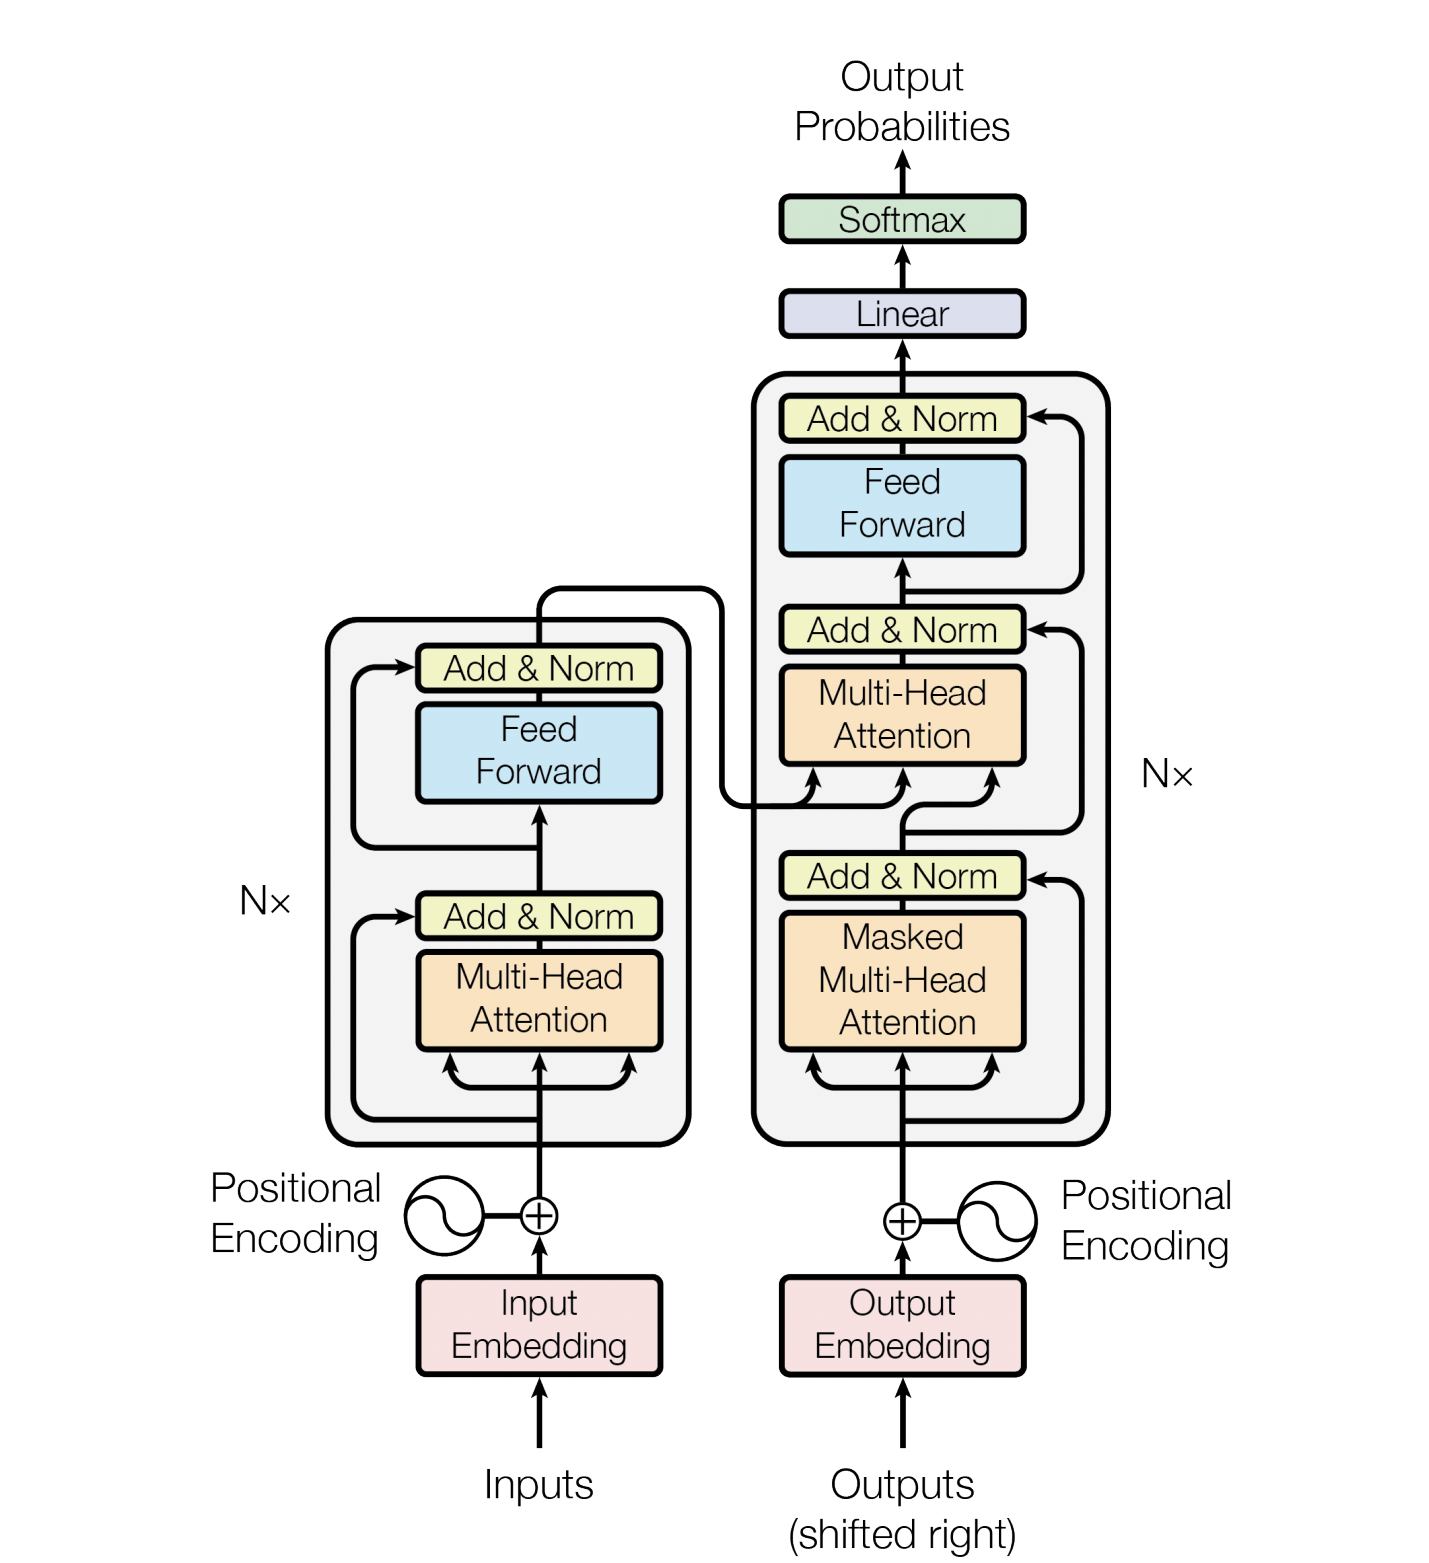
\includegraphics[width=0.9\textwidth]{images/transfo-arch.png}
    \caption{The Transformer architecture as proposed by \citet{vaswani2017attention}. We can see the encoder (left) and decoder (right) stacks and their interconnection.}
    \label{fig:trafo}
\end{figure}
The Transformer architecture is another neural network architecture capable of processing sequential data.
It was first proposed in \citet{vaswani2017attention}.
Unlike RNNs, the Transformer architecture does not work with a hidden state that is being passed forward in time.
Instead, the architecture is based solely on the attention mechanism, which allows the model to learn long-range dependencies between different parts of the input sequence.
The high-level equation describing the self-attention mechanism is formulated as follows:
\begin{equation*}
    Att(Q,K,V) = softmax\left(\frac{QK^T}{\sqrt{d_k}}V\right)
\end{equation*}
where $Q$, $K$ and $V$ are trainable square weight matrices corresponding to \emph{queries}, \emph{keys} and \emph{values} and with dimension $d_q$, $d_k$, $d_v$ respectively.
The attention mechanism allows the model to focus on different parts of the input sequence when producing the output sequence.
For example, if the model is translating a sentence from English to German, the attention mechanism can allow the model to focus on the English words most relevant to the German words that need to be produced.

The original Transformer architecture comprises an encoder and a decoder, depicted in Figure~\ref{fig:trafo}.
The encoder takes the input sequence and produces a sequence of hidden representations.
The decoder then takes these hidden representations and produces the output sequence.
The attention mechanism is used at both the encoder and decoder to allow the model to use different parts of the input sequence when producing the output sequence.
The decoding process might be autoregressive or non-autoregressive, depending on the use case.

Both the encoder and decoder are a stack of self-attention layers.
Each self-attention layer takes the hidden representations from the previous layer and produces a new set of hidden representations.

The decoder also includes an attention component that allows the model to attend to the output sequence generated so far when producing the next token.
This allows the model to learn how to generate the output sequence consistently with the input sequence and the prefix generated so far.

The Transformer architecture has been shown to achieve state-of-the-art results on various natural language processing tasks. 
Moreover, the Transformer architecture was used as a base for many models pre-trained on large natural language corpora, allowing efficient transfer of the learned information to downstream tasks and thus revolutionizing the NLP field.

\section{pre-trained Language Models (PLMs)}
\label{background:plms}
The appearance of PLMs marked a new era in NLP.
Although Language Modeling with neural networks has been in the community focus for some time with transforming works such as  \citet{mikolov2010recurrent,mikolov2013distributed}, it was not until RNN-based models such as ELMo \cite{peters-etal-2018-deep} and ULMFiT \cite{howard-ruder-2018-universal} were proposed that we were able to create PLMs that could be fine-tuned for a variety of tasks with comparably low data requirements.

Shortly after ELMo, models based on the Transformer architecture started to appear, such as BERT for efficient language encoding \cite{devlin2019} or GPT for generation \cite{radford2018improving}.
BERT introduced a novel approach to Transformer usage by employing only the encoder part of the original Transformer architecture.
Importantly, BERT pre-training introduced the task of Masked Language Modeling, randomly masking some of the input tokens and reconstructing them correctly at the output.
Additionally, BERT is trained to estimate the probability that two input sentences follow each other.
These pre-training techniques make BERT great at encoding natural language inputs into useful representations.
GPT, on the other hand, consists only of Transformer decoder blocks.
It is trained for next token prediction and can perform autoregressive Language Modeling.
Therefore, GPT is a perfect candidate for a base model to be fine-tuned on language generation tasks, including data-to-text, summarization, etc.


Both BERT and GPT showed great potential for fine-tuning downstream tasks and established themselves as strong baselines for many NLP tasks and benchmarks.
They are often referred to as \emph{foundational} models because of their language understanding and generation abilities and the potential to apply these abilities to various tasks.
From a certain point of view, the usability of PLMs lies in the ability to create useful and contextual representations of input words and phrases, often called \emph{(word) embeddings}.
This ability has been observed in the word2vec model \cite{mikolov2013distributed} and improved by ELMo~\cite{peters-etal-2018-deep}, BERT~\cite{devlin2019}, SBERT~\cite{reimers2019sentence} and others.

Many model architectures based on Transformer blocks followed both for encoders \cite{liu2019roberta,reimers2019sentence}; decoders \cite{radford2019language,brown2020language} or even encoder- decoder~\cite{raffel2020exploring,lewis-etal-2020-bart}.
The NLP community largely adopted these models.


\subsection{Large Language Models (LLMs)}
The foundational models changed the NLP paradigm but still need substantial in-domain data to perform some tasks well.
Moreover, fine-tuning those larger models requires more computational resources.
Therefore, more lightweight methods were proposed to adapt the models to downstream tasks, such as Transformer Adapters \cite{pfeiffer2020AdapterHub}.
However, as researchers started to scale up the models with GPT-2 and GPT-3 leading the efforts \cite{radford2019language,brown2020language}, new abilities emerged \cite{wei2022emergent}.
With model sizes exceeding billions of parameters, the large pre-trained Transformer decoders can perform many tasks that they were not explicitly trained for \cite{brown2020language}.
Such large models can perform tasks like summarization, translation, question answering, or even reasoning and arithmetics to some extent without any task-specific training.
However, it is unclear how many examples of the abovementioned tasks were seen during these models' training phase.
Those tasks can be presented to the LLMs purely in the form of textual task descriptions in the inference time.
This approach of \emph{in-context learning} is frequently used with great success \cite{min2022rethinking,dong2022survey}.
The textual input for LLMs is frequently called a \emph{prompt}.

\paragraph{On LM scaling}
Scaling laws in language models describe the relationship between the size of a language model and its performance.
It has been shown that with the next token prediction objective (which is what virtually all LMs are trained for), some abilities start to emerge when exceeding a certain size threshold \cite{kaplan2020scaling}.
However, bigger models also need to be trained longer and with more data \cite{hoffmann2022training}.
In general, larger language models tend to perform better than smaller models but also require more computational resources to train.
This line of research can help us understand how the size of a language model affects its performance and predict the performance of a language model before it is trained.

\paragraph{Instruction Tuning}
Although the LLMs have great abilities and potential to accomplish various tasks, providing them with correct instructions is not always straightforward.
Therefore, significant effort was made to \emph{align} the LLMs better with the human requirements.
Consequently, even rather inexperienced users can instruct the model to accomplish custom tasks according to their needs.
For this purpose, reinforcement learning techniques were explored \cite{ziegler2019fine,ouyang2022training}.
Although these techniques proved to be quite effective, the process is still very demanding in collecting user feedback.
Consequently, several datasets were proposed \cite{supernaturalinstructions,black2022gpt} that contain tasks like summarization, reasoning, etc. formulated using instructions in natural language and desired outputs.
These datasets allow tuning of the models using reinforcement learning or supervised fine-tuning methods.

\paragraph{Prompt engineering vs. LLM fine-tuning}
\label{02:in-context}
The in-context learning approach has great advantages because it makes it possible to obtain great performance from LLMs by simply formulating the task and desired output structure in the LLM input (i.e. prompt).
There are multiple strategies to formulate the prompt of the in-context learning technique.
We can include examples for better model guidance or just formulate the instructions.
These approaches are referred to as \emph{few-shot} or \emph{zero-shot} settings, respectively.
Although this approach might be very efficient for some tasks, especially those that are well described in the corpora available to the LLM during training \cite{wei2022emergent}, some more specific tasks might yield better results after fine-tuning of the model \cite{tu-etal-2022-prompt}.
However, the LLM fine-tuning process is quite demanding regarding computational resources.
Therefore, alternative approaches were proposed, such as LoRA \cite{hu2021lora} or Transformer Adapters \cite{pfeiffer2020AdapterHub}.
These approaches make LLM fine-tuning much more accessible.
In general, fine-tuning and in-context learning can offer great performance and be beneficial in certain situations~\cite{mosbach-etal-2023-shot}.

\section{Variational autoencoders}
\label{02:sec:vae}
In neural network training, the network learns to create internal data representations to accomplish a given task.
In the case of autoencoders, the task is to encode an input $\mathbf{x}$ in a way that allows for its reconstruction into the original form.
The autoencoder model consists of an encoder function $\varphi^{enc}$, which encodes an input $\mathbf{x}$ into a latent representation $\mathbf{z}$, and a decoder $\varphi^{dec}$, which models the conditional re-generation probability $p(\mathbf{x}|\mathbf{z})$.
In the case of sequence autoencoders, both the encoder and decoder can be realized with an RNN.
However, vanilla autoencoders often fail to extract global semantic features of natural language sequences \cite{bowman2015generating}; therefore, adjustments must be made to obtain better representations.
The technique proposed by \citet{kingma2013auto} uses the Variational Autoencoder (VAE) framework to tackle this issue.
The architecture is modified so that $\varphi^{enc}$ represents a recognition model $q(\mathbf{z}|\mathbf{x})$ which parameterizes an approximate posterior distribution over $\mathbf{z}$.
Figure~\ref{fig:vae-vs-ae} illustrates the differences.
VAEs impose prior distribution on the latent variable $\mathbf{z}$, which acts as regularization during training and makes drawing samples from $q$ possible.
Consequently, the VAE latent space is smooth because it is possible to interpolate between two points and obtain reasonable representations.
The latent space structure is depicted schematically in Figure \ref{fig:vae}.
The modeled distributions are typically Gaussian; the prior is the standard normal distribution $N(0, 1)$.
\begin{figure}[t]
    \centering
    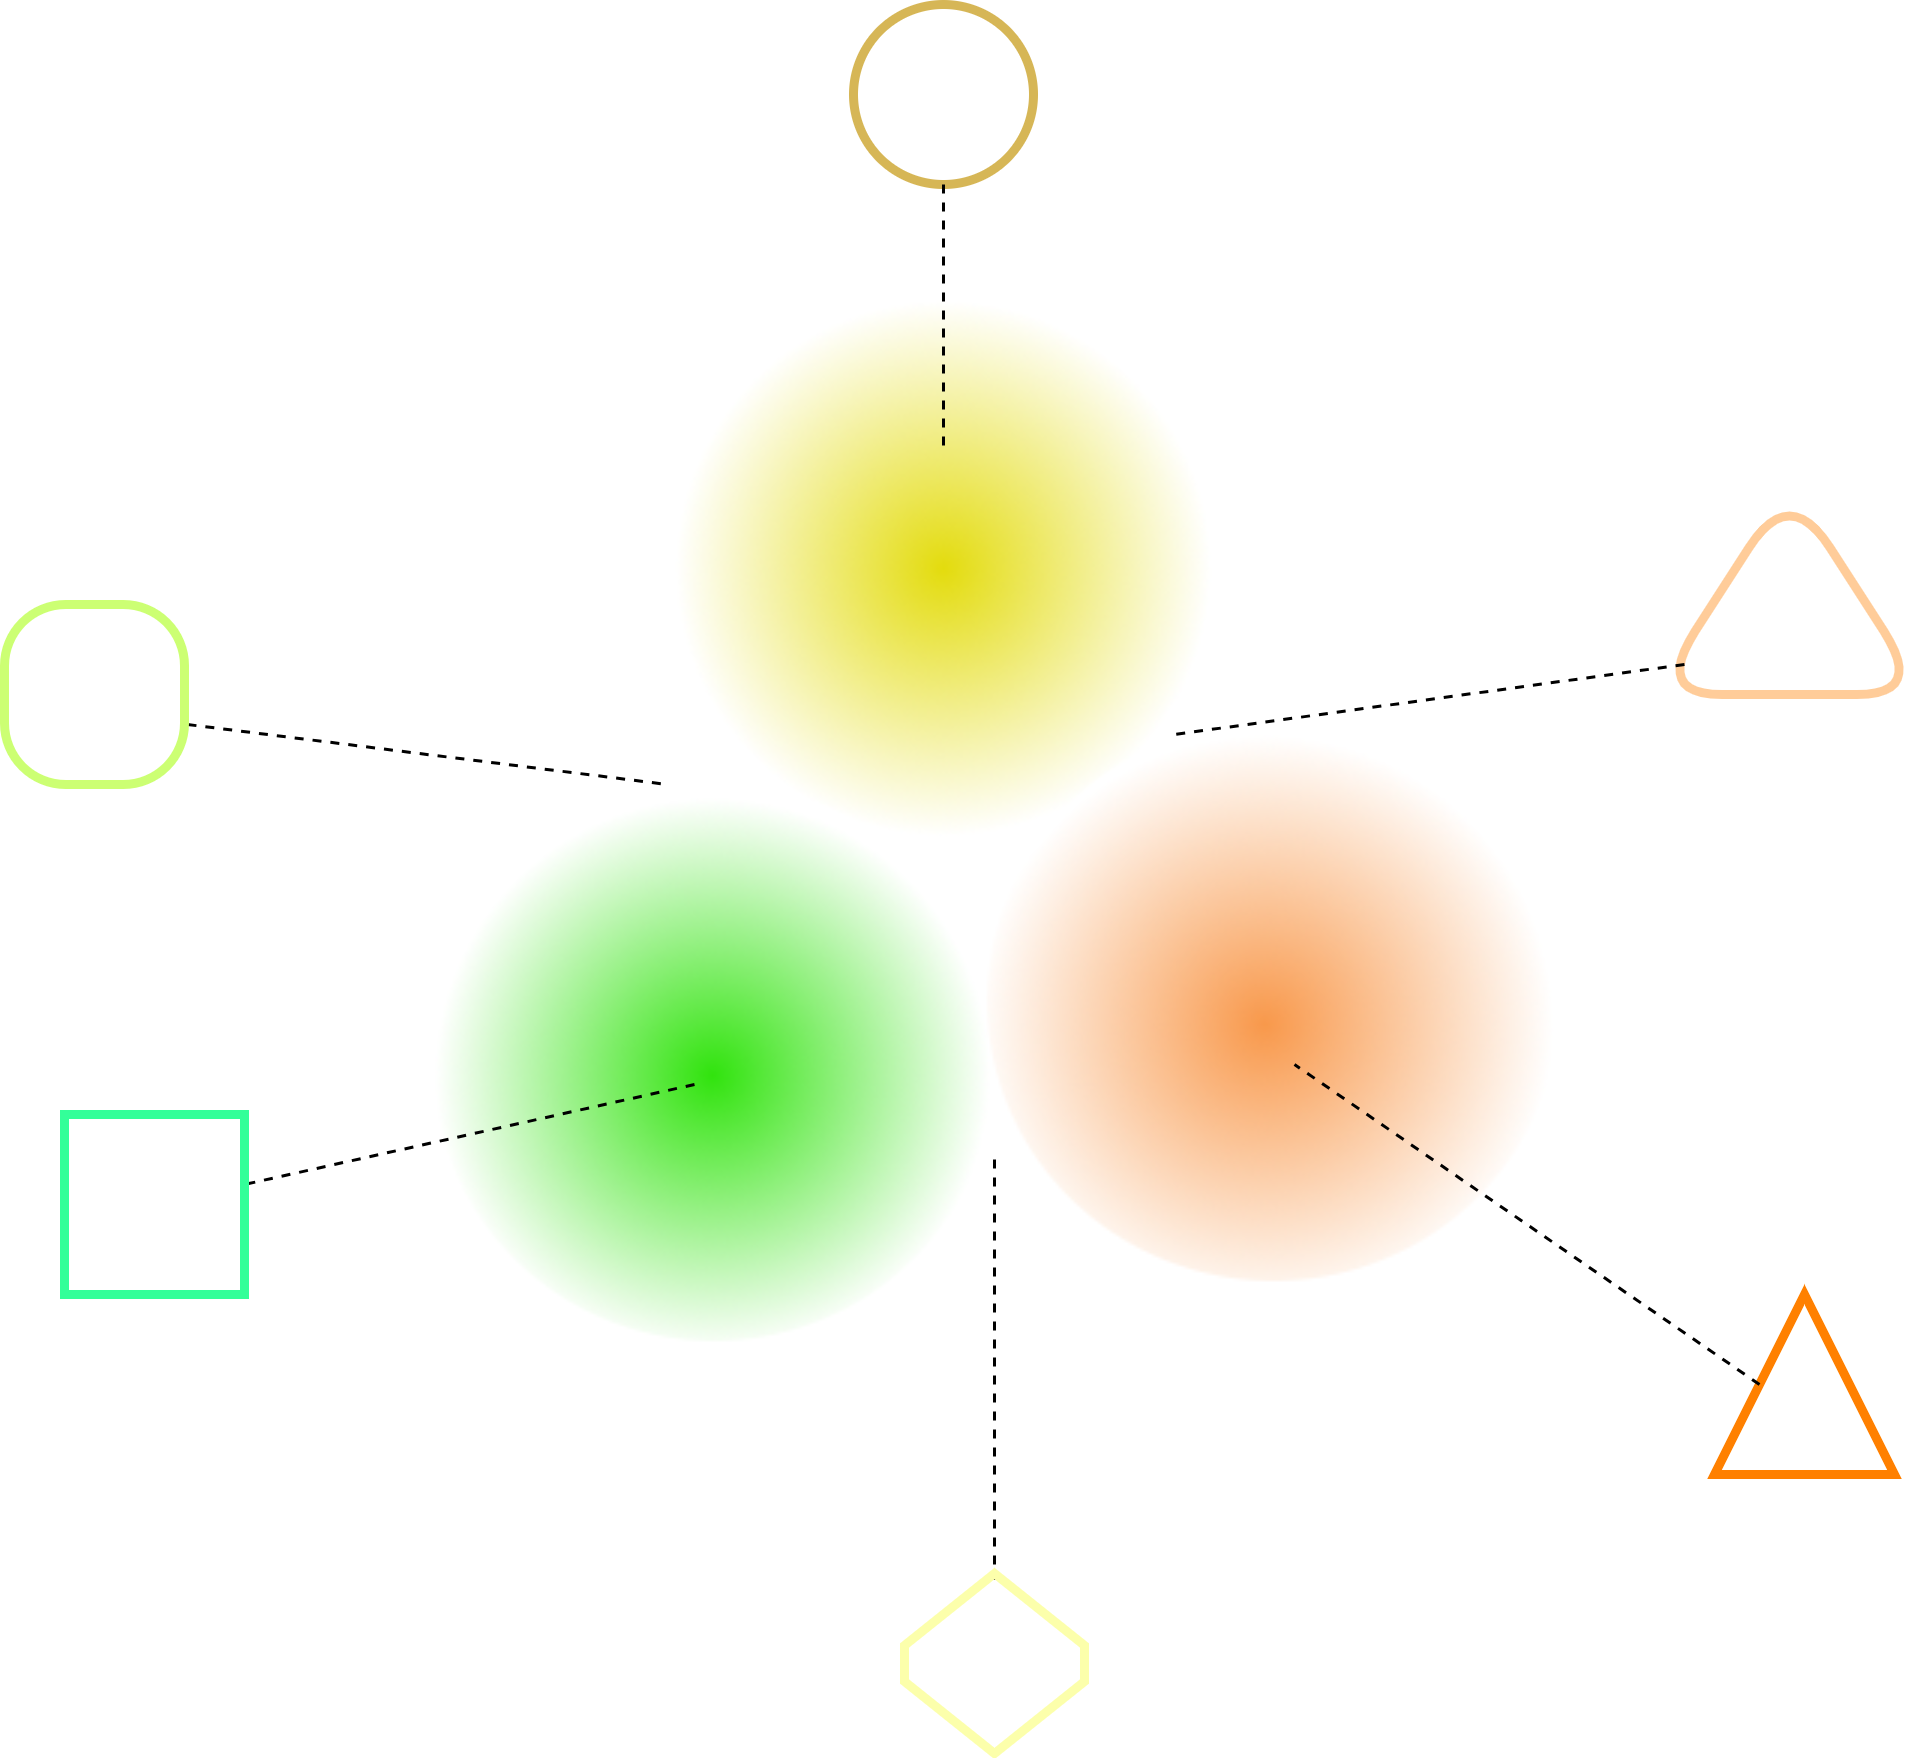
\includegraphics[width=0.46\textwidth]{images/VAE.png}
    \caption{Variational autoencoder latent space. Colors and different classes by shapes distinguish the encoder distributions. It illustrates that we can interpolate between two points in the latent space smoothly.}
    \label{fig:vae}
\end{figure}
\begin{figure}[t]
    \centering
    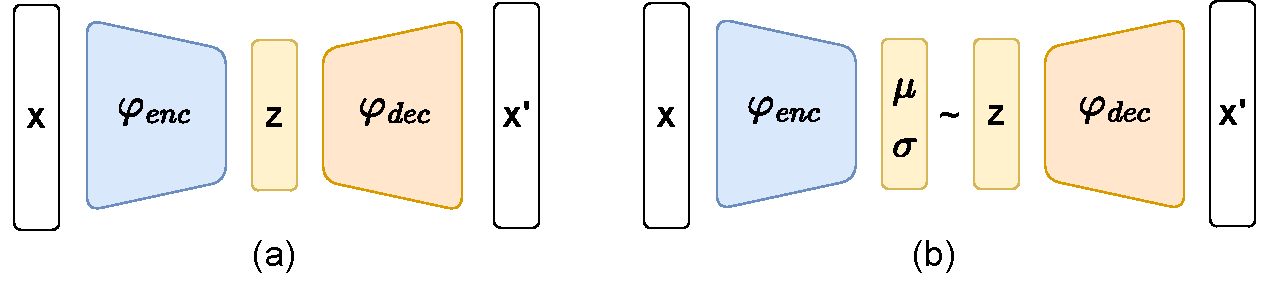
\includegraphics[width=0.9\textwidth]{images/enc-dec.pdf}
    \caption{Illustration of differences between the architectures of a vanilla autoencoder (a) and its variational version (b). The VAE encodes the input by predicting parameters of probabilistic distribution from which the data are drawn rather than encoding the data directly into a hidden representation, as done with the vanilla autoencoder.}
    \label{fig:vae-vs-ae}
\end{figure}
We can realize the encoder and decoder modules in VAE using neural networks.
However, there is a drawback regarding the implementation of sampling.
The sampling operation is not differentiable and, therefore, cannot be trained using standard approaches.
A solution to this problem is to use the \textit{reparameterization trick} \cite{kingma2013auto}.
The reparameterization trick exploits that a random variable under a certain conditional distribution can be expressed as a deterministic transformation of some other variable with an independent marginal distribution.
Distributions that allow us to do such a transformation include \textit{Gaussian, Logistic}, or \textit{Gumbel}~\cite{jang2016categorical}.

\subsubsection{VAE latent space discretization}
\label{02:sec:vae_discrete}
Although VAE training yields robust representations that are also more interpretable thanks to the regularized latent space, in some cases, we require the latent representations to be discrete.
The motivation is mainly to improve interpretability and uncover underlying processes in sequential tasks.
Incorporating discrete variables into neural network models is problematic because the widely used backpropagation algorithm requires smooth differentiable functions to propagate the gradients correctly.
\citet{van2017neural} propose a vector quantization technique to discretize the latent variables in VAEs.
Another approach is to use the Gumbel-softmax distribution \cite{jang2016categorical} that, together with the reparameterization trick (Section \ref{02:sec:vae}), enables working with categorical variables while not breaking the gradient flow in the network.

\subsection{Variational Recurrent Neural Networks}
\label{02:sec:vrnn}
\begin{figure}
    \centering
    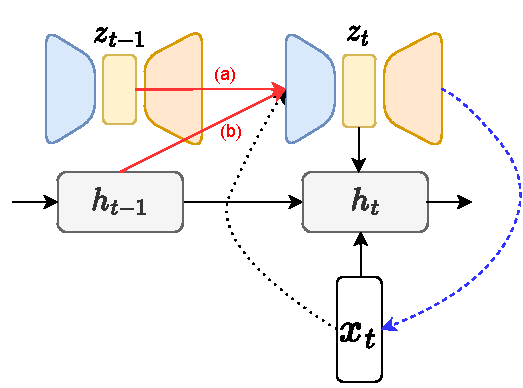
\includegraphics{images/DVRNN.pdf}
    \caption{A schematic architecture of the VRNN model. The input in time step $t$ is input to the variational autoencoder (black dotted line). The VAE prior is conditioned either on the previous hidden state (a) or previous latent variable $z_{t-1}$ (b) (red lines). To regenerate the output, the decoder from latent space is used (blue dashed line). Finally, the hidden state update is based on latent representation $z_t$, previous hidden state, and current input (solid black lines).}
    \label{fig:DVRNN}
\end{figure}
The VRNN model \cite{chung2015recurrent} exploits the idea of variational training to model sequences with latent states.
Intuitively, the VRNN model can be seen as a recurrent network with a VAE in every timestep.
The VRNN architecture is depicted in Figure~\ref{fig:DVRNN}.
It assumes that the sequence of observations was generated from a sequence of unknown latent states and uses a VAE to model these latent variables $\mathbf{z}$.
Formally, we want to estimate the joint probability distribution of a sequence of observations and corresponding latent variables $p(\mathbf{x}, \mathbf{z}) = p(\mathbf{x}|\mathbf{z})p(\mathbf{z})$.
The conditional distribution $p(\mathbf{x}|\mathbf{z})$ is parameterized with a neural network.
However, we still need to estimate the posterior $p(\mathbf{z}|\mathbf{x})$ to connect the latent variables with the observations.
The VAE uses a variational approximation $q(\mathbf{z}|\mathbf{x})$ that allows maximizing the evidence lower bound (ELBo) of the log-likelihood of the data:
\begin{equation}
\begin{split}
    \log~p(\mathbf{x}) \ge -\mathrm{KL}(q(\mathbf{z}|\mathbf{x})||p(\mathbf{z}))\\ + \mathbb{E}_{q(\mathbf{z}|\mathbf{x})}[\log~p(\mathbf{x}|\mathbf{z})]
    \label{eq:vae}
\end{split}
\end{equation}
where KL is the Kullback-Leibler divergence.

We consider a prior network $\varphi_{prior}$ and a posterior network $\varphi_{post}$, which compute the parameters of $p(\mathbf{z})$ and $q(\mathbf{z}|\mathbf{x})$ respectively.
In a VRNN, $\varphi_{prior}$ and $\varphi_{post}$ additionally depend on the RNN hidden state $\mathbf{h}^t$ to allow for a context-aware prior distribution.
In each time step, we obtain the distribution parameters as follows:
\begin{equation}
\label{eq:distr_theta}
\begin{gathered}
    \mathbf{\theta}_{q}~=~\varphi_{post}(\mathbf{h}^t, \varphi_{enc}(\mathbf{x}^t))\\
    \mathbf{\theta}_{p}~=~\varphi_{prior}(\mathbf{h}^t)
\end{gathered}
\end{equation}
where $\varphi_{enc}$ is the encoder and $\theta_q, \theta_p$ are parameters of the respective distributions.
With distribution parameters available, we can sample the latent variable and predict the output:
\begin{equation}
\label{eq:x_infer}
\begin{gathered}
    \mathbf{z}^t~\mathtt{\sim}~p(\mathbf{z};\theta_{p})\\
    \mathbf{x}^t~=~ \varphi_{dec}(\mathbf{z}^t)
\end{gathered}
\end{equation}
where $\varphi_{dec}$ represents the decoder network.
The update of the hidden state $\mathbf{h}^t$ is as follows:
\begin{equation}
    \label{eq:hidden_update}
    \begin{gathered}
        \mathbf{h}^{t+1} = \text{RNN}([\varphi_{enc}(\mathbf{x}^t),\varphi_{z}(\mathbf{z}^t)], \mathbf{h}^t)
    \end{gathered}
\end{equation}
where $[.,.]$ is concatenation, $\varphi_z(.)$ is a feature extractor, and $\text{RNN}()$ is a step transition function of a recurrent neural network, in our case an LSTM \cite{hochreiter1997}.

\subsection{Latent Action Spaces via Variational Auto-encoding -- LAVA}
\label{02:sec:lava}
\todo{More details}
The LAVA framework~\cite{lubis-etal-2020-lava} focuses on learning latent variables in a way that they store dialogue-related actions.
To achieve this, they employ VAE-based model architecture.
The architecture comprises an RNN utterance encoder, VAE module, and RNN decoder.
They train the model in multiple stages and different variants.
Specifically, they first pre-train the encoder module using an autoencoding objective.
Then, they use the pre-trained decoder and train an additional encoding module for the next response prediction.
In the end, they use reinforcement learning to tune the model parameters further.
Formally, the authors first train an encoder-decoder network with an autoencoding objective version of ELBo parameterized by $\phi$.
\begin{equation}
    \mathbb{L}_{ae}(\phi) = \mathbb{E}_{q_{\phi}(\mathbf{z}|\mathbf{x})}[\log~p_{\phi}(\mathbf{x}|\mathbf{z})] -\mathrm{KL}(q_{\phi}(\mathbf{z}|\mathbf{x})||p(\mathbf{z}))
\end{equation}
where $\mathbf{x}$ represents dialogue utterance.
Then, they train the response generation network parameterized by $\theta$ using the lite ELBo objective~\cite{lubis-etal-2020-lava}.
\begin{equation}
    \mathbb{L}_{lite}(\theta) = \mathbb{E}_{q_{\theta}(\mathbf{z}|\mathbf{c})}[\log~p_{\theta}(\mathbf{x}|\mathbf{z})] - \beta\mathrm{KL}(q_{\theta}(\mathbf{z}|\mathbf{c})||p(\mathbf{z}))
\end{equation}
where $\mathbf{c}$ is a sequence of utterances representing the dialogue context.
For the second step, the decoder network $p_{\theta}$ is initialized by pre-trained $p_{\phi}$.

\subsection{Difficulties of the VAE training}
\label{background:vae-problems}
For text VAEs~\citep{bowman-etal-2016-generating}, the KL divergence term measured between the posterior and prior distributions often tends to zero.
Consequently, the modeled latent space degrades, and the latent variables do not contain useful information.
This phenomenon is called posterior collapse, where the model ignores the latent variables and solely focuses on the decoder for maximum likelihood estimation.
To address this issue, several modifications were proposed.
A common approach is to use \emph{warm-up} or \emph{annealing schedules}~\cite {fu-etal-2019-cyclical}.
In this method, the weight of KL divergence in the loss function starts at zero and gradually increases to its maximum value over several epochs.
This allows the decoder to learn useful information before the encoder starts learning the prior.
Another method is called \emph{free bits}~\cite{li2019surprisingly}.
This method decouples the optimization of the likelihood and the KL term.
Each dimension in the latent space can use a fixed capacity (bits) to encode the data before the KL term is minimized.

\section{Memory Networks}
\label{02:sec:mem_nn}
\begin{figure}[t]
    \centering
    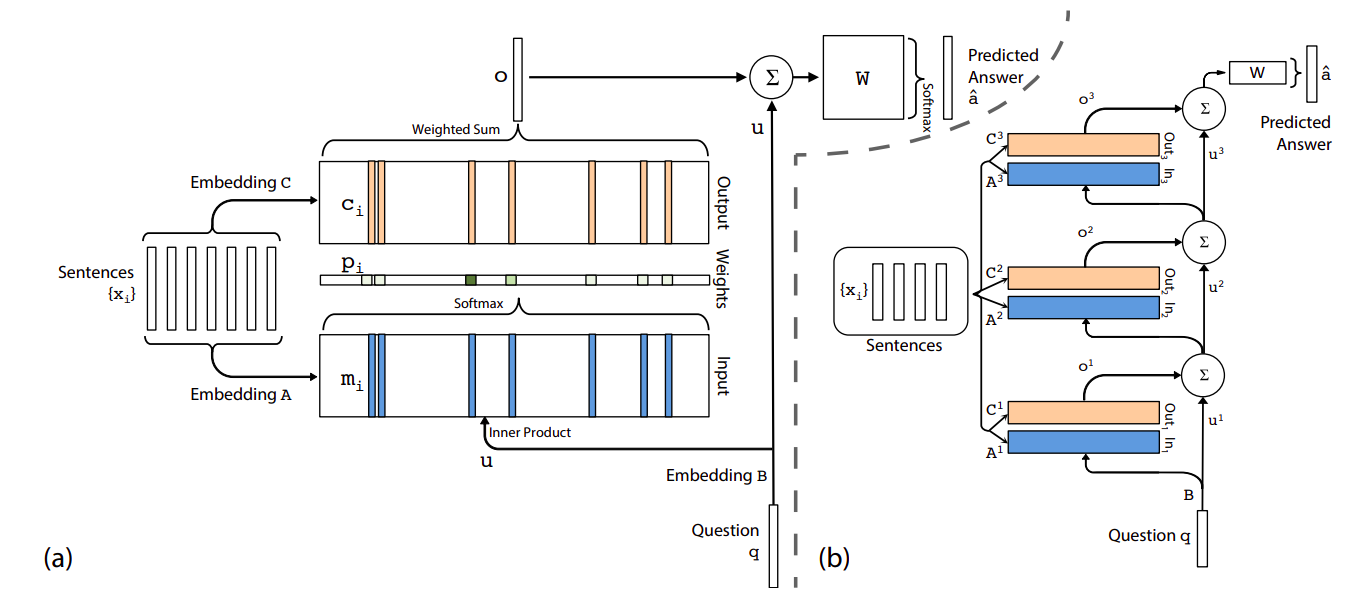
\includegraphics[width=\textwidth]{images/e2e_mem_nn.png}
    \caption{The end-to-end Memory Network model introduced in \citet{sukhbaatar2015end}. It shows the computation process of (a) a single-layer and (b) a 3-layer model version. }
    \label{fig:e2e_memnn}
\end{figure}
The Memory Network model (MemNN) addresses the issue associated with RNN networks, which typically suffer from catastrophic forgetting and exponential decay of stored information \cite{neil2016phased}.
The Memory Network model was originally introduced in \citet{DBLP:journals/corr/WestonCB14}.
\subsection{The Memory Network architecture}
The key idea behind memory networks is to incorporate an external memory component into the network architecture, allowing the model to store and access information over long sequences of inputs.
The memory component acts as a separate storage module, similar to a computer's memory, which the network can read from and write to during its computation.
The MN model architecture's main component is a memory array $\mathbf{m} = \{\mathbf{m}_1,...,\mathbf{m}_n\}$.
The basic Memory Network takes an input $\mathbf{x}$ and processes it in four processing steps:
\begin{enumerate}
    \item The input $x$ is processed with \emph{input feature map} $I$ to obtain internal representations of the input $I(x)$.
    \item The memory array is updated using the \emph{generalization component} $G$. In this step, each memory entry gets updated following the equation $\mathbf{m}_i = G(\mathbf{m}_i, I(\mathbf{x}), \mathbf{m})$.
    \item The output features are computed with the \emph{output feature map} using the memory and transformed input $ o = O(I(\mathbf{x}, \mathbf{m}))$
    \item Finally, the output representation is used to decode the final response: $r = R(o)$
\end{enumerate}

The components $I, G, O$, and $R$ can be represented with any function capable of doing the task.
However, in most cases in the literature, we see models that use neural networks to instantiate these components.
Consequently, the whole model is end-to-end differentiable and thus trainable with algorithms such as backpropagation.
In that case we talk about Memory Neural Networks (MemNNs).
Although various kinds of data can be input and output to MemNNs in general, we consider only MemNNs that work with text in this work.
Let us describe a basic MemNN for text.
When given text input, such a basic model can save each text memory into a new memory slot.
Therefore, old memories are not updated, and new inputs are stored sequentially.
The most interesting components of this simple text model are $O$ and $R$.
The $O$ module scores the saved memory vectors given text input $x$ and subsequently retrieves $k$ supporting entries with the highest scores from the memory.
The $R$ module takes the input $x$ and $k$ retrieved memories to produce a response.
It generates an output by copying one of the memories or creating new outputs, for example, with an auto-regressive RNN decoder. 

\subsection{Multi-hop end-to-end MemNN}
The MemNN architecture's disadvantage is that it requires supervision at each layer during training, as pointed out by \citet{sukhbaatar2015end}.
In this work, the authors address this problem and present a fully end-to-end trainable memory network model, which we call \emph{e2e MemNN}.
In the e2e MemNN, we input a set of vectors $x$ to be stored in the memory and a query $q$.
Each input $x_i$ is then embedded with two distinct embedding functions $E_m$ and $E_c$ to obtain a memory entry $m_i$ and corresponding output embedding $c_i$, respectively.
The query $q$ is then embedded with the different function $E_q$ to obtain query embedding $u$.

\begin{figure}[t]
    \centering
    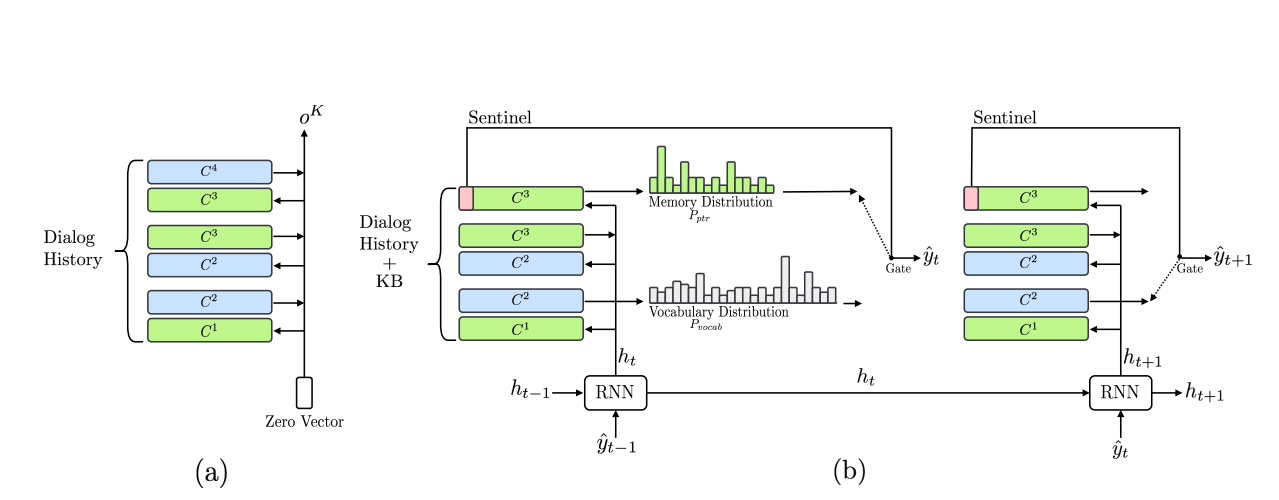
\includegraphics[width=\textwidth]{images/mem2seq.png}
    \caption{The Mem2Seq model \cite{madotto-etal-2018-mem2seq} showing the memory encoder with 3 hops (a) and 2 steps of the memory decoder (b) }
    \label{fig:mem2seq}
\end{figure}

Upon embedding the inputs, a memory distribution $p$ is computed as a match between $u$ and each memory $m_i$ as $\operatorname{softmax} (u^Tm_i)$.
The memory distribution $p$ is then used to create an output $o$ computed as a weighted sum over the output embeddings $\sum_i p_ic_i$.
The output $o$ is then used to produce the final answer, a categorical label or textual response generated with an auto-regressive model.

The authors also introduce a multi-layer version of this model.
In the multi-layer version, each layer $k$ has distinct embedding matrices $E^k_m$ and $E^k_c$. The output $o_k$ from layer $k$ is used to form input query embedding $u_{k+1}$ to the layer $k+1$: $u_{k+1} = u_k + o_k$.
The multi-layer processing is sometimes referred to as \emph{multi-hop} where a \emph{hop} refers to processing by one layer.

\subsection{Mem2Seq model}
\label{02:sec:mem2seq}
The Mem2Seq model \cite{madotto-etal-2018-mem2seq} is a task-oriented dialogue model that builds on top of the end-to-end architecture introduced in \citet{sukhbaatar2015end}.
The architecture is described in Figure \ref{fig:mem2seq}.
The model consists of encoder and decoder parts.
The encoder is a 3-hop memory network that encodes the dialogue context.
The more interesting part is the decoder, a recurrent neural network enhanced with a memory network in every time step.
This memory network contains conversation history and knowledge base entries encoded as memory vectors.
At each step, the hidden state of the RNN is used as a query vector. Then, a distribution over memory is computed, as described earlier. 
Also, a distribution over vocabulary is computed from the RNN hidden state, similar to standard RNN-based decoders.
One special entry is added to the memory, so-called \emph{sentinel}.
The vocabulary distribution generates the next token if the highest probability is assigned to the sentinel token.
Otherwise, the next token is chosen according to the memory distribution.
In other words, the model uses the RNN state at each generation step to decide whether to copy something from memory (conversation history + knowledge base info) or generate an arbitrary new token from vocabulary distribution.
This way, the model can use information from the past effectively.

\section{Dialogue System implementations}
\label{02:ds-background}
\begin{table*}[tp]
\small
\setlength\fboxsep{2pt}
        \centering
        \begin{tabular}{rll}
        \textbf{\texttt{USER:}} & \textit{\texttt{I would like a cheap restaurant.}} & \textbf{\texttt{\colorbox{pastelyellow}{inform}(\colorbox{lightblue}{price}=\colorbox{pastelgreen}{cheap})}} \\
        \textbf{\texttt{SYSTEM:}} & \textit{\texttt{Golden plate is cheap.}} & \textbf{\texttt{\colorbox{pastelyellow}{inform}(\colorbox{lightblue}{name}=\colorbox{pastelgreen}{Golden plate})}} \\
        \hdashline[1.5pt/2pt]
        \textbf{\texttt{USER:}} & \textit{\texttt{What is the cuisine?}} & \textbf{\texttt{\colorbox{pastelyellow}{request}(\colorbox{lightblue}{cuisine})}} \\
        \textbf{\texttt{SYSTEM:}} & \textit{\texttt{They serve chinese food.}} & \textbf{\texttt{\colorbox{pastelyellow}{inform}(\colorbox{lightblue}{cuisine}=\colorbox{pastelgreen}{chinese})}} \\
        \hdashline[1.5pt/2pt]
        \textbf{\texttt{USER:}} & \textit{\texttt{Sounds good. Bye!}} & \textbf{\texttt{\colorbox{pastelyellow}{goodbye}()}} \\
        \textbf{\texttt{SYSTEM:}} & \textit{\texttt{Have a great day.}} & \textbf{\texttt{\colorbox{pastelyellow}{goodbye}()}} \\
        \end{tabular}
\normalsize
        \caption{Example of task-oriented dialogue in the restaurant reservation domain. Utterance representations as dialogue acts are depicted on the right. Intents are highlighted in orange, slot names in blue, and respective values in green. Note that not all dialogue acts include slots and values.}
    \label{fig:das}
\end{table*}
First, we describe various approaches to constructing dialogue systems pipelines and provide insights about approaches to modeling the underlying processes.
The architectures may vary greatly because of the varying use cases of Dialogue Systems (DS).
We thus introduce a classification of dialogue systems that reflects the expected capabilities.
There are multiple approaches to defining a dialogue system taxonomy in the literature.
Here, we introduce the widely used classification scheme \cite{jurafsky2000speech}.
\begin{enumerate}
    \item \textbf{Question Answering (QA)} - Although sometimes not mentioned in the context of dialogue systems, the QA task can be seen as a simple conversation. A QA system's main task is to answer the user's questions.
    The topics may vary; good understanding and knowledge representation are essential for this task.
    The dialogues are usually quite simple and often consist of just one question and the respective answer.
    \item \textbf{Task-oriented DS} - In this setting, the system's goal is to complete a task based on the user's instructions.
    The successful completion may depend on several attributes the system has to learn from the user utterances.
    The system is also allowed to ask for additional information if needed and typically works with some external source of information, such as a database.
    Here, the dialogues are usually much more complex than in the QA setting, and dialogue context has to be considered.
    \item \textbf{Chit-chat} - Sometimes, we might be interested in a system that can talk to the user casually and provide entertainment.
    Such systems might be combined with task-oriented systems to serve as human-like virtual assistants or use the dialogue to advertise products, etc.
    The context and knowledge base are also important, but in most cases, there is no well-defined task to be completed, so the evaluation is subjective.
\end{enumerate}

Another way of classifying the dialogues considers their domain of operation.
\textbf{Single-domain} systems can work only in one topic area, e.g. public transport or restaurant information, whereas \textbf{multi-domain} systems can handle multiple domains.
These types of systems cannot give meaningful answers outside the domains they are trained on.
A dialogue system is considered \textbf{open-domain} if it can have a conversation not limited to a predefined set of domains.
In practice, this is achievable only to some extent since the knowledge base of the program is always limited.
However, the systems can cover many domains with internet access and smart information retrieval methods.

Here, we focus on the task-oriented DS and discuss it more deeply.
From the domain perspective, task-oriented DS are usually single or multi-domain systems.
Open-domain dialogue systems are rare, at least in the research community.
We can see a task-oriented dialogue as a composition of two tasks - slot-filling and response generation.
Task-oriented dialogue systems are widely used for various applications, such as customer service, personal assistance, and information retrieval. These systems aim to assist users in accomplishing specific tasks by engaging in a natural language conversation. 
That means we have a predefined set of semantic \textit{slots} that must be filled with the right \textit{values}.
Each utterance in the task-oriented dialogue is considered an action that potentially changes the state of the conversation.
Such actions can be represented using \textit{Dialogue Acts (DA)}~\cite{core1997coding}.
To define the Dialogue Act, we first must introduce the concept of \emph{slots} and \emph{intents}.
To represent the meaning of user utterances, annotation based on \emph{slots} is commonly employed \cite{young_pomdp-based_2013}. Slots, which describe semantic concepts relevant to completing the task, serve as a means of capturing the user's desires as well as facilitating the system's communication with the user. Typical examples of slots include \emph{area}, \emph{price}, and \emph{address}, among others. By tracking slots and their values throughout the dialogue, a dialogue system can maintain a \emph{dialogue state}, effectively planning the next actions \cite{williams2013dialog}. The dialogue state represents explicitly all the important knowledge known to the system at a specific point in the dialogue. Consequently, it can be utilized to communicate with external sources of information and data, such as databases, structured knowledge bases, or various APIs, to provide users with accurate and relevant information.
Intent describes the user's intention expressed by a respective utterance.
In other words, intent represents what the user wants and what their wish is.
Slots describe attributes of this wish and ground it to an ontology.

DA is a tuple consisting of an \textit{intent} and \textit{slot} and the corresponding \textit{value}.
If multiple slot values are present, all are considered to have the same intent.

An example dialogue with respective DA representation is depicted in Table \ref{fig:das}.
Most dialogue system modules for limited domains can be implemented by designing a set of rules and templates.
Such systems can yield satisfying results in some use cases.
Nevertheless, they are inflexible and generally not considered promising from the research point of view.

\subsection{Dialogue System Architectures}
\begin{figure}[t]
    \centering
    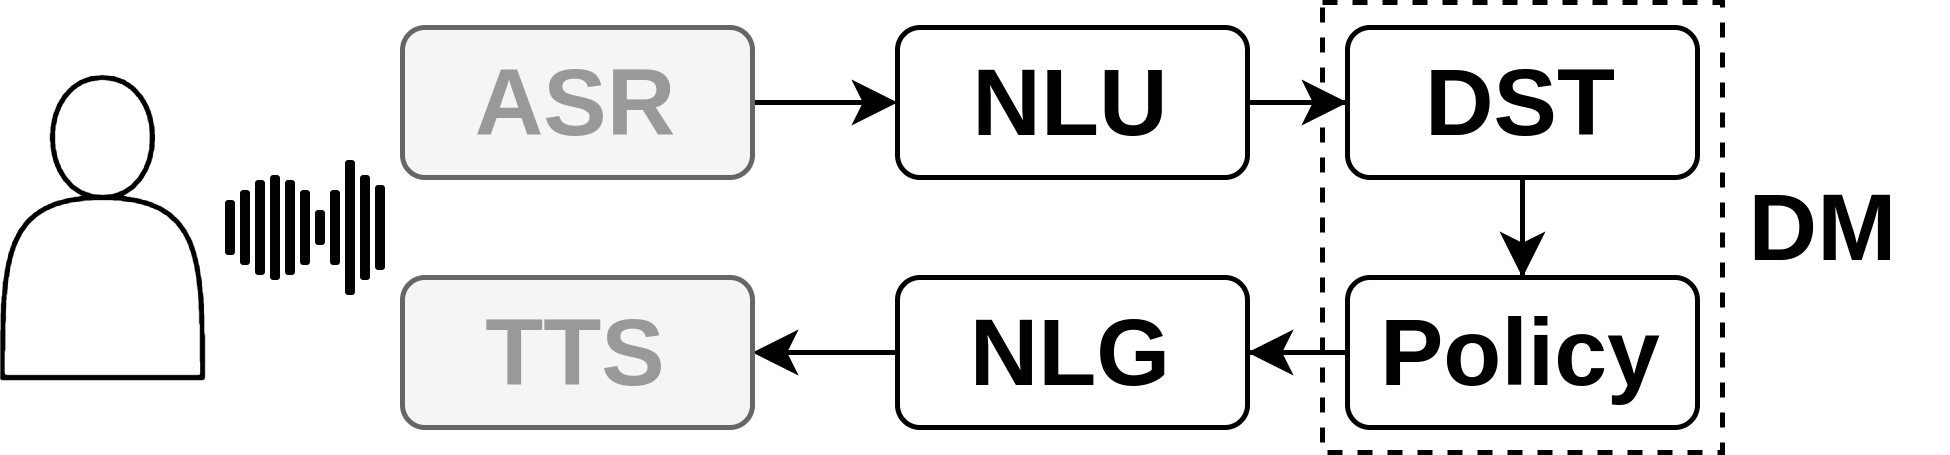
\includegraphics[width=0.80\textwidth]{images/pipeline.png}
    \caption{Overall architecture of task-oriented dialogue system pipeline. The data flow is outlined with arrows. This work does not discuss ASR and TTS modules (depicted in gray), often included with the rest of the components.}
    \label{fig:overall}
\end{figure}
A typical approach to task-oriented DS implementation is to create a modular system with several modules that handle the conversation flow together.
An example of such architecture is depicted in Figure \ref{fig:overall}
We shortly discuss the responsibilities of each component:
\begin{itemize}
    \item \textbf{Natural Language Understanding (NLU)} The purpose of NLU is to extract the meaning of input utterances in natural language and transform it into a structured representation, i.e., dialogue acts.
    Basically, the NLU module has three subtasks.
    (1) It has to determine the domain of the utterance, (2) detect the user intent, and (3) capture any slot values, if present.
    \item \textbf{Dialogue State Tracking (DST)} Dialogue state keeps track of the dialogue history, effectively providing the necessary context.
    Dialogue State Trackers update the state with correct values after each turn.
    \item \textbf{Dialogue Policy} The core component of the DS is the dialogue policy.
    Its responsibility is to decide which action the system should take at each turn.
    In other words, Dialogue Policy's responsibility is to guide the dialogue to follow the desired path.
    Dialogue policy and the DST component are sometimes called \emph{Dialogue Manager}.
    \item \textbf{Natural Language Generation (NLG)} When the decision on a system action is made, the system needs to verbalize the action.
    In other words, we need to create an utterance in natural language that expresses the information in the system's underlying representation.
\end{itemize}

The module-based approach is advantageous thanks to its good level of explainability.
In case of low performance, we can track the respective modules' outputs and find the source of problems.
On the other hand, error accumulation makes it difficult to recover from errors made by the modules early on in the pipeline.
Another disadvantage is the way these systems are trained \cite{li-etal-2017-end}
Each component requires specific data annotation.
Thus, obtaining a dataset suitable for training all components can be difficult and costly.
Also, the system design itself is more complicated since it requires the implementation of multiple models.
Because of the drawbacks, many current research works focus on dialogue modeling end-to-end, i.e., using systems without explicit components that can be trained jointly.
\label{02:delex}
One of the commonly used concepts in end-to-end dialogue modeling is that of \emph{delexicalization} \cite{wen-etal-2015-stochastic}.
When using delexicalization, the slot values in the text of the utterances are replaced by placeholders.
This addresses the problem of data sparsity because the model can learn just the important concepts and does not have to remember full ontology or use the correct values.
Also, delexicalized values are better suited for interaction with external interfaces -- we can fill (lexicalize) them later in a deterministic way to prevent the model from hallucinating incorrect values.
However, delexicalization also suffers from several drawbacks.
First, it is not straightforward to perform and requires ontology knowledge.
Second, the inverted lexicalization process is sometimes difficult to implement and might require complex rules.

\subsection{Modeling TOD without supervision}
\label{02:no-super}
Here, we introduce some challenges concerning TOD modeling without external structured supervision.
We discuss every step in the pipeline (Section~\ref{02:sec:basics}) separately.

\paragraph{Natural Language Understanding (NLU)}
Recall that the purpose of the NLU component in a traditional dialogue pipeline is to extract the meaning from input utterances in natural language and represent it in a structured way.
Doing this unsupervised is challenging because we do not have the labeled data for training and do not know the structure itself in the first place.
However, there are some possible ways to approach this problem.
Works focus on automated annotation schema induction (\ref{sec:relwork-unsup}).
Another way is to let the model handle NLU implicitly, i.e., effectively omitting the NLU step.

\paragraph{Action Selection}
One of the tasks of the dialogue manager is to select the next system action in a given situation.
Most implemented systems implicitly perform this task, i.e., there is no explicit representation of the system action, just a surface realization (verbalized utterance).
The reason for this option is that it requires less supervised labels, which might be hard and costly to obtain.
However, modeling the information about system action can benefit the overall performance~\cite{DBLP:conf/aaai/LiangTCY20}.
We explore the possibility of implicitly learning this information by introducing a network bottleneck in Chapter~\ref{chap:modeling}.

\paragraph{Handling external interfaces}
Task-oriented dialogue systems must provide accurate and complete information based on user requests, which requires interaction with external interfaces such as databases or some structured knowledge base.
To communicate with such external entities, we typically need to design some representation with a predetermined structure so we can construct API queries, etc.
This can be troublesome in a setting where no supervision in the form of labels is present.
Without a known structure, it is very challenging to design the communication protocol with external sources of information.

\subsection{Modeling a dialogue with Language Models (LMs)}
\label{background:2stage-lm-modeling}
\begin{figure}[h]
    \centering
    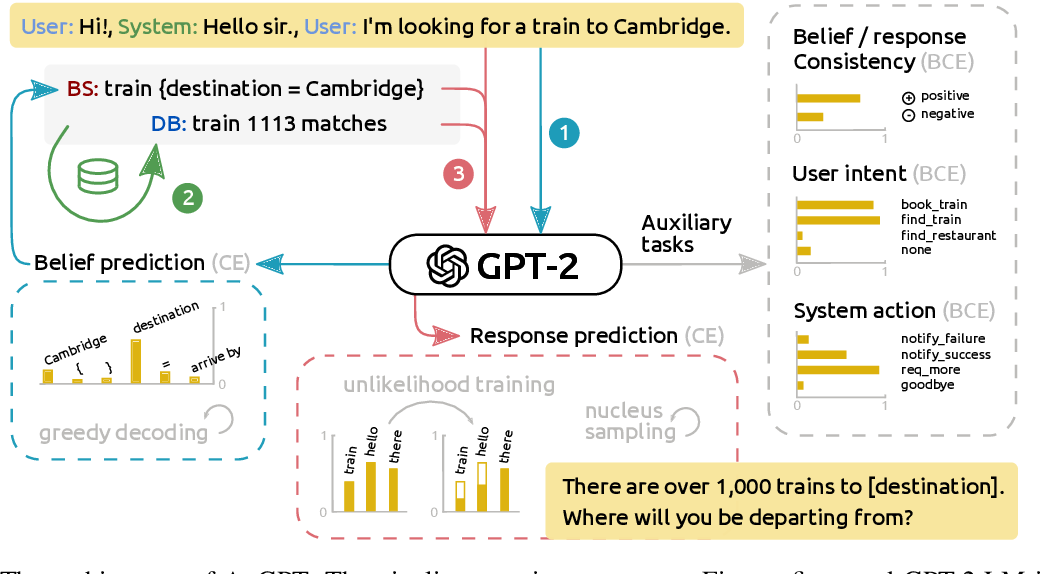
\includegraphics[width=\textwidth]{images/augpt.png}
    \caption{An explanation of two-stage LM-based dialogue model as described in \citep{kulhanek-etal-2021-augpt}}
    \label{fig:augpt-2-stage}
\end{figure}
The pre-trained LMs can generate fluent and natural-sounding text and work with structured data.
It is desirable to leverage these properties for end-to-end dialogue modeling.
However, it's not a straightforward application.
Task-oriented dialogues require interaction with external interfaces, so there is a need to have some intermediate structured representation 
to allow this interaction.
A common approach (depicted in Figure~\ref{fig:augpt-2-stage}), pioneered in \citep{lei2018sequicity}, proposes to split the generation into two steps: (1) belief state generation and (2) response generation.
This allows us first to decode a structured representation that can be used to interact with external interfaces and extend the context.
In the subsequent step, the model has all the needed information in the input and can generate the final response.

\section{Datasets}
\label{02:sec:input-data-desc}
We describe some of the most prominent datasets we use for our experiments.
Most of them are largely used in the dialogue community and provide common benchmarks used for the evaluation.
All these datasets have several task-oriented dialogue characteristics that define the conversation according to \cite{young_pomdp-based_2013}:
\begin{enumerate}
\item \textbf{Domain(s)} define the topic (or range of topics) which are mentioned in the dialogue. There can be several domains per dialogue.
\item \textbf{Task}: the users in each dialogue attempt to reach a certain goal (such as booking a restaurant or finding a tourist attraction).
\item \textbf{Turns} We consider \emph{turn-taking} dialogues, i.e.\ the participating sides exchange utterances alternately.
One such utterance exchange is called a dialogue turn.
Utterance is considered the linguistic realization of the speaker's thoughts and will. It can be spoken or written. 

The meaning of each utterance can be represented in a structured way with \textbf{Dialog Act(s)} \cite{Weisser2016}.
It is a meta-information that emerges from the respective utterance and qualifies it. It describes the beliefs, desires, and intentions.
Dialogue acts can be represented using \emph{Domains}, \emph{Intents}, and \emph{Slots} as described in Section~\ref{02:ds-background}.
The slots can also be further categorized.
Typically, we define \emph{inform} and \emph{request} slots (Table~\ref{02:tab:inf-req}). Inform slots correspond to information provided by the user and inform about constraints the user has, while request slots communicate the kind of information that the user wants to obtain.
\begin{table}[tp]
    \centering
    \begin{tabular}{l|l}
    \toprule
         \textbf{User} & \texttt{I am looking for a {\color{cyan!80!yellow!80!black!100 } Chinese} restaurant} \\
         \textbf{System} & \texttt{The Golden Dragon is a nice place in the South} \\
         \textbf{User} & \texttt{Please, give me their {\color{orange!50!yellow!90!black!100!}phone number} and {\color{orange!50!yellow!90!black!100!}address}} \\
         \bottomrule
    \end{tabular}
    \caption{An illustration of the difference between {\color{cyan!80!yellow!80!black!100 }\textbf{inform}} and {\color{orange!50!yellow!90!black!100!}\textbf{request}} slots.}
    \label{02:tab:inf-req}
\end{table}
The intent represents the user's intention, i.e., the sub-goal that the user wants to achieve with a particular utterance.
For an example of dialogue act annotation, we refer to Figure~\ref{fig:das} in Section~\ref{02:ds-background}.
Slots represent the attributes that instantiate the dialogue act.
Each domain is associated with certain intents; each intent can be combined with multiple slots. A slot, however, can be used by multiple intents as well.
We provide statistics about the dialogue datasets we use in this work in Table \ref{02:tab:data_stats} and some samples in Tables \ref{02:tab:mw_example} and \ref{02:tab:smd_example}.
\end{enumerate} 

\subsection{Datasets description}
\label{02:sec:data-desc}
\paragraph{MultiWOZ} (\textbf{MW}) is an established task-oriented dataset introduced by \citet{budzianowski-etal-2018-multiwoz}.
It has been released in several versions; the standard most commonly used nowadays are MultiWOZ 2.1 and MultiWOZ 2.2.
MultiWOZ 2.2 is a version of the original dataset improved by (1) fixing some annotation errors, inconsistencies, and ontology issues and (2) adding slot span annotations for utterances.
MultiWOZ contains over 10,000 annotated dialogues and spans multiple domains -- restaurant and hotel reservations, tourist attraction search, and taxi and train reservations.
While some of the dialogues use only a single domain, most of them are multi-domain.
For example, after finding a restaurant, the user also asks for a hotel and orders a taxi.
This makes the dataset more relevant to real-world use cases.

The data were gathered via a crowd-sourcing Wizard-of-Oz scheme described in~\citet{wen-etal-2017-wizard-of-oz}.
As MW is used most in our work, we provide further information on the data distribution in Figure~\ref{02:fig:mw-dist} and a sample of the data in Table~\ref{02:tab:mw_example}.

\paragraph{DSTC2} \cite{henderson_robust_2014} was introduced as a part of a challenge to improve state tracking within dialogue systems. It contains over 3,000 dialogues covering a single domain around restaurant reservations. The dialogue corpus was collected using Amazon Mechanical Turk\footnote{\url{https://www.mturk.com/}} with a POMDP-based spoken dialogue system. It is the only human-machine dataset in our collection.

\paragraph{CamRest676} (\textbf{CR}) \cite{wen2016network} is another crowd-sourced dialogue corpus gathered via the Wizard-of-Oz scheme. CamRest676, with its 676 conversations, is the smallest of the datasets used in this work, and it is also a single-domain dataset focused on helping users to find a restaurant in Cambridge, UK. 

\paragraph{Schema-guided dialogue} (\textbf{SGD}) is a large (more than 20,000 dialogues) multi-domain (around 20 domains covered) dataset containing a total of 45 API services based on a pre-defined schema. First, the data was collected via a simulator that interacts with the API services, and then the dialogues were paraphrased using crowd-sourcing. \\

\paragraph{ATIS} (\textbf{AT}) \cite{hemphill_atis_1990} contains utterances taken from conversations about flight searches and reservations. \footnote{There are multiple ATIS data versions available. We used one from \url{https://www.kaggle.com/siddhadev/atis-dataset-from-ms-cntk}.}

\paragraph{Cambridge SLU} (CS) \cite{henderson2012discriminative} resembles the CamRest 676 dataset but is larger and focuses only on other user parts of the conversations.
Therefore, Cambridge SLU is not a true dialogue dataset as it contains only single utterances and can be used solely for the NLU task.

\paragraph{Stanford Multidomain Dialogues} (\textbf{SMD}) \cite{eric-etal-2017-key} contains concise dialogues between a driver and an in-car virtual assistant about appointments, navigation, and weather.
The dataset assumes interaction with the database or external APIs.
However, the information is provided with each dialogue in the form of relevant Knowledge Base entries.
We provide an example from the data in Table~\ref{02:tab:smd_example}.

\subsection{Dataset limitations}
\label{02:sec:data-limits}
Although the number of dialogue datasets is quite big, and there is arguably a lot of variance with respect to the size, data collection approach, etc. there are some limitations that are inherently present with this type of data.
We want the data to be used for two main purposes: training and evaluation.
Both these aspects are influenced by the static nature of the data.
Dialogue is a dynamic process that requires interaction.
Hundreds of alternatives exist for a conversation representing a certain information exchange with different phrasing, length, or turn ordering.
All of this is impossible to capture in a static dataset.
Therefore, dialogue modeling should somehow consider this.
A similar issue stems from the fact that there are multiple valid responses under a specific dialogue context, not only with respect to the phrasing but also considering dialogue acts.
Consequently, model evaluation with these data tends to penalize generated responses that are meaningful and relevant but do not correspond to the ground truth found in the data.

Another consideration regards the focus of these datasets.
We almost exclusively work with \emph{task oriented} datasets in this work.
Therefore, the instances contain some structured annotation, most frequently in a dialogue state.
While this addresses the above-mentioned issues to some extent, the conversations usually lack variability and do not exhibit user behavior like repetitions, small talk, clarifications, hesitation, etc.
Therefore, there is a substantial gap with respect to real-world data distribution.
On the other hand, the other type of dialogue datasets tries to exhibit these properties but lacks any structure.
Recently, some efforts were made to join these two approaches \cite{sun-etal-2021-adding}.

\begin{table}[tp]
    \centering\footnotesize
    \begin{tabular}{l@{\hspace{0.8em}}r@{\hspace{0.3em}}r@{\hspace{0.3em}}r@{\hspace{0.3em}}r@{\hspace{0.3em}}r@{\hspace{0.3em}}r@{\hspace{2em}}r}
        \toprule
        \textbf{Data}         & \textbf{SGD} & \textbf{MW} & \textbf{DSTC} & \textbf{CR} & \textbf{SMD} & \textbf{ATIS} & \textbf{Total} \\ \midrule
        \textbf{Domains}        & 18        &    7        &      1        &      1  & 3 & 1  &    19$^{\ast}$ \\
        \textbf{Slots}        & 145       &    29       &     10        &      7    & 15 &  79 & 166$^{\ast}$ \\
        \textbf{Dialogues$^{\ast\ast}$}       & 22.8    & 10.4     &    3.2     &      0.7    & 3 & -- & 37.1\\
        \textbf{Turns$^{\ast\ast}$}        & 463.3   & 143.0     &    51.0  &     5.5   & 16.1 & 4.9 & 662.8\\
        \textbf{Turns/Dial.}   & 20.30     & 13.71       &   15.77        &     8.12   & 5.25 & -- & 17.83 \\
        \textbf{Avg. utt. length} & 9.86      &  13.23      &   8.47        &  10.71     & 9 & 11.37  & 10.49 \\
        \textbf{Unique Words}$^{\ast\ast}$ & 32.3 & 23.2 & 1.3 & 1.7   & 1.6 & 0.9 & 49.9 \\

     \bottomrule
    \end{tabular}
    \caption{Basic statistics of the datasets we use in this work. Overall and for individual sources (number of domains and slots, total numbers of dialogues and turns, average number of turns per dialogue, and average utterance length in terms of words. Due to ontology overlap, $^{\ast}$ is not a sum. $^{\ast\ast}$ in thousands.}
    \label{02:tab:data_stats}
\end{table}

\begin{table}[tp]
    \centering
    \begin{tabular}{l|l}
    \toprule
         \textbf{User} & \texttt{I need to book a hotel in the {\color{cyan!80!yellow!80!black!100 }east} that has { \color{orange!50!yellow!90!black!100!}4 stars.}} \\
         \textbf{System} & \texttt{I can help you with that. What is your price range?} \\
         \textbf{State} & \texttt{restaurant \{\}, ..., hotel \{"area": "{\color{cyan!80!yellow!80!black!100 }east}", "stars": "{\color{orange!50!yellow!90!black!100!}4}" \}} \\
         \textbf{User} & \texttt{That does not matter as long as it has {\color{cyan!80!yellow!80!black!100 } wifi} and {\color{orange!50!yellow!90!black!100!}parking}.}\\
         \textbf{System} & \texttt{If you'd like something cheap, I recommend the Allenbell.} \\
         \textbf{State} & \texttt{restaurant \{\}, ..., hotel \{"area": "east", "stars": "4",}\\
         & \texttt{"wifi": {\color{cyan!80!yellow!80!black!100}yes}", "parking": "{\color{orange!50!yellow!90!black!100!}yes}"\}} \\
         & \texttt{...} \\
         \bottomrule
    \end{tabular}
    \caption{A simplified example taken from the MultiWOZ corpus. It shows a snippet from a conversation between the customer and the agent about booking a hotel. It also shows this corpus' annotation schema for tracking belief state.}
    \label{02:tab:mw_example}
\end{table}


\begin{table}[tp]
    \centering
    \begin{tabular}{l|l}
    \toprule
         \textbf{Driver} & \texttt{What {\color{cyan!80!yellow!80!black!100}gas stations} are here?} \\
         \textbf{NLU} & \texttt{\{"poi\_type": "{\color{cyan!80!yellow!80!black!100}gas stations}" \}} \\
         \textbf{Car} & \texttt{There's a Chevron} \\
         \textbf{Driver} & \texttt{That's good! Please pick the {\color{cyan!80!yellow!80!black!100}quickest} route }\\ & \texttt{to get there and {\color{orange!50!yellow!90!black!100!}avoid all heavy traffic}!} \\
         \textbf{NLU} & \texttt{\{"distance": "{\color{cyan!80!yellow!80!black!100}quickest}",} \\
            & \texttt{"traffic\_info": "{\color{orange!50!yellow!90!black!100!}avoid all heavy traffic}"\} }\\
         \textbf{Car} & \texttt{Taking you to Chevron} \\
         \midrule
         \textbf{KB} & \texttt{"items": [} \\
          & \texttt{    \{"distance": "5 miles",} \\
          & \texttt{    "traffic\_info": "moderate traffic",} \\
          & \texttt{    "poi\_type": "gas station",} \\
          & \texttt{    "address": "783 Arcadia Pl",} \\
          & \texttt{    "poi": "Chevron"\}} \\
          & \texttt{    ...} \\
          & \texttt{]} \\
          \bottomrule
    \end{tabular}
    \caption{A simplified example taken from the SMD corpus with utterance-level annotations. Compared to MultiWOZ, some of the slot values are open, such as "avoid all heavy traffic"}
    \label{02:tab:smd_example}
\end{table}
\begin{figure}[ht]
    \centering
    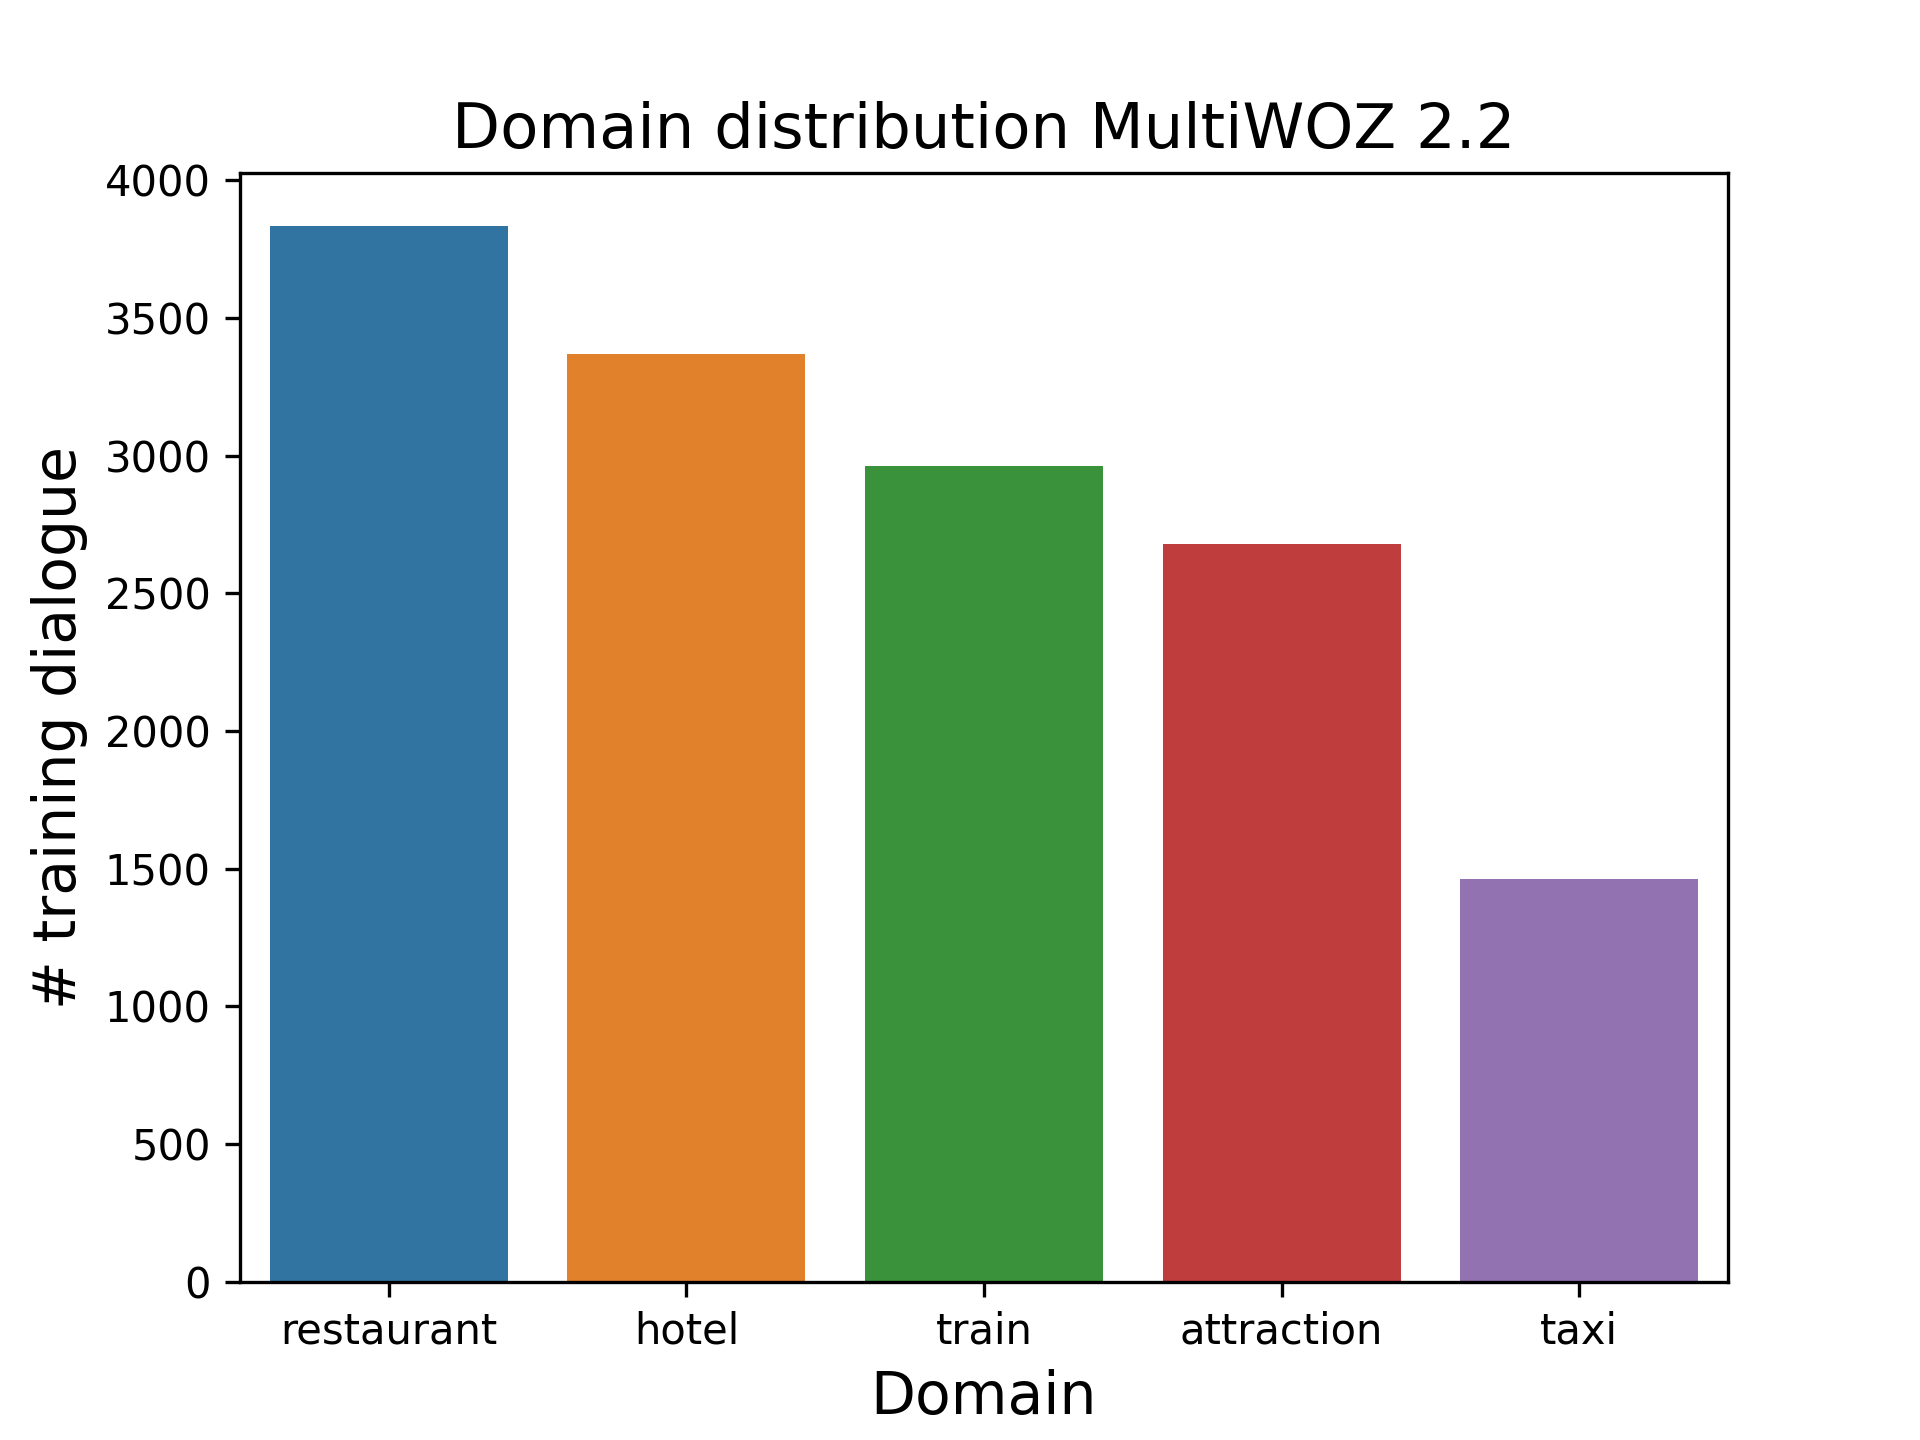
\includegraphics[width=0.8\textwidth]{images/multiwoz-distribution.png}
    \caption{The distribution of respective domains in the MultiWOZ dialogue dataset, showing how many of the dialogues contain the respective domain.}
    \label{02:fig:mw-dist}
\end{figure}


\section{Evaluation metrics}
\label{02:sec:eval_metrics}
Here, we provide a set of commonly used metrics to evaluate the quality of dialogue modeling and response generation.
We also use some less common metrics for specific tasks.
Those metrics are described together with experiments in respective sections of this work.
\subsection{NLU metrics}
    \begin{itemize}
        \item \textbf{$F_1$ Score} (F-score, F-measure)~\cite{goutte2005probabilistic} is a widely used metric to evaluate binary classification.
    To measure F1 score, we first compute the number of occurrences of True Positives (TP), False Positives (FP), and False Negatives (FN).
    Subsequently, we can compute Precision (P) and Recall (R) in the following way:
    \begin{equation*}
        P = \frac{TP}{TP + FP}; R = \frac{TP}{TP + FN}
    \end{equation*}
    The $F_1$ score is then computed as a harmonic mean of P and R:
    \begin{equation*}
        F_1 = \frac{2\cdot P \cdot R}{P + R}
    \end{equation*}
    $F_1$ score is sometimes used also to measure multiclass classification performance.
    Usually, two ways of $F_1$ generalization are used. \emph{Micro $F_1$ score} averages per-class $F_1$ scores with weights corresponding to the respective class frequencies whereas \emph{Macro $F_1$ score} considers all classes equally important.
    $F_1$ is a classification evaluation metric task, and in the context of dialogue NLU it is frequently used to evaluate the performance of slot filling.
        \item \textbf{Intent Accuracy} is the percentage of slot occurrences assigned into the correct intent cluster under the reference mapping.
        \item \textbf{Domain Detection Accuracy} is simply the ratio of cases in which the system correctly detects the domain.
        \item \textbf{Entity Match Rate (EMR)}~\cite{wen2016network} calculates the last turn's entity in each dialogue. Using the final constraints, it verifies if a correct entity would be retrieved from the database.
    \end{itemize}
\subsection{State tracking metrics}
    \begin{itemize}
    \item \textbf{Joint Goal Accuracy (JGA)}~\cite{mrkvsic2016neural} is computed as the ratio of dialogue turns for which the predicted belief state matches the ground truth.
    We use fuzzy matching of the slot values so that capitalization or minor typos do not influence the result.
    \item $F_1$ score on the slot level can also be used to evaluate the performance of state tracking.
    \end{itemize}
\subsection{Dialogue-level metrics}
    \begin{itemize}
        \item The main \emph{overall measure} for evaluating a task-oriented dialogue is the dialogue \textbf{success rate} \cite{deriu_survey_2021}.
For MultiWOZ, we use the standard evaluation of dialogue success as the ratio of dialogues where the user reaches the desired goal, based on goal annotation provided with the data \cite{nekvinda-dusek-2021-shades}. 
The SGD dataset does not include goal annotation but contains information about the requested slots. Therefore, we compute SGD success rate as the proportion of dialogues in which (1) the system captures all the informed slots correctly and (2) all the requested slots are provided.
For more details about the inform and request slots, we refer the reader to Section~\ref{02:sec:input-data-desc}.
    \item  \textbf{BLEU score} \cite{papineni-etal-2002-bleu} is largely used to evaluate response generation in machine translation, summarization, and other tasks, including dialogue generation.
    Although it has some flaws \cite{callison-burch-etal-2006-evaluating} and was designed mainly for corpus-based evaluation, it is widely used, so it is desirable to measure it for comparison with other works.
\end{itemize}

There are multiple different criteria for dialogue systems evaluation.
In the case of modular systems, the individual modules can be evaluated separately.
It is considerably harder to measure a system's overall performance.
The policy module's decision is difficult to evaluate without turn-level action annotations.
BLEU usage is controversial for dialogue systems since it often fails to capture the semantics of the utterance, which is perhaps more critical than in the translation task \cite{lowe2017towards}.
It is also common to measure \textbf{Dialogue success rate}.
However, it is not straightforward how to define dialogue success robustly.
Many systems use user simulators to allow the employment of reinforcement learning techniques.
In such scenarios, the user behavior is model-based and can be non-deterministic. Therefore, defining success is challenging.
Usually, it is based on evaluating user and system dialogue acts, which rely on good and extensive data annotation.

\subsection{Human Evaluation}
Due to the mentioned challenges, \textbf{human evaluation} remains the best way to evaluate dialogue systems.
Human evaluation plays a crucial role in developing and refining dialogue systems. Automated tools or metrics often fail to capture human communication's nuanced responses and language variations. 

Dialogue systems, including chatbots and virtual assistants, are directly designed for human interaction, making their performances depend heavily on how effectively they can understand and respond.
Therefore, assessing their capabilities requires a human-like understanding of the conversations.

Moreover, human evaluation is important to measure aspects beyond the correctness of the system's responses. For instance, the engagingness of the conversation or the appropriateness of the system's tone requires human judgment. Also, human evaluators can better identify and evaluate cultural and social aspects than automated methods.

While human evaluations are more time-intensive and costlier than automated ones, they offer a more detailed, insightful, and accurate assessment of the dialogue system's performance.
Therefore, they are crucial for improving these systems to make them more user-friendly and effective for human interaction.
% %%%%%%%%%%%%%%%%%%%%%%%%%%%%%%%%%%%%%%%%%%%%%%%%%%%%%%%%%%%%%%%%%%%%%%%%%%%%
\chapter{Related Work}%
\label{chap:related}
% %%%%%%%%%%%%%%%%%%%%%%%%%%%%%%%%%%%%%%%%%%%%%%%%%%%%%%%%%%%%%%%%%%%%%%%%%%%%
\label{sec:relwork}

\subsection{Modular dialogue architectures}
\label{relwork:modular}
The traditional dialogue system implementation, especially for task-oriented dialogues, is based on modular architecture.
The modular system consists of several components connected to form a pipeline.
First, the Natural Language Understanding (NLU) module parses the utterance and creates structured representation.
Based on NLU outputs, the dialogue management module determines the next action.
Dialogue Management usually consists of the state tracker that updates state based on NLU outputs and the policy module that chooses the action.
Finaly, the language generation module is used to verbalize the chosen action.
\subsubsection{Natural Language Understanding (NLU)}
From the machine learning point of view, the intent and domain detection can be seen as a classification task and sentence-level classification can be utilized \cite{yaman2008integrative,schapire2000boostexter}.
The slot-value filling can be approached as a sequence tagging problem.
Many approaches have been proposed to tackle this issue, ranging from SVM \cite{shi2016recurrent} and HMM \cite{surendran2006dialog} based taggers to various neural models \cite{adel2016comparing, zhang2017position, mesnil2014using}.
Because of the similar nature of these three sub-tasks, it is reasonable to model them jointly.
Especially modeling the intent detection together with slot filling proved to be beneficial for the model performance \cite{zhang2017position, liu2016attention, xu2013convolutional}.

\subsubsection{Dialogue State Tracking (DST)} 
\label{relwork:DST}
The most straightforward solution to this problem is a rule-based system that simply tracks the current slot values based on NLU.
However, the situation is usually more complicated.
We need to take into account a distribution of slot value probabilities and the update rules can be rather complex.
\citet{vzilka2013comparison} provides a comparison of different data-driven models for dialogue state tracking.
Neural networks have also been used to model the distributions \cite{mrkvsic2016neural, zhong2018global} and deal with multiple domain handling \cite{rastogi2017scalable}.

\subsubsection{Dialogue Policy}
\label{relwork:policy}
The policy decision can thus be framed as a classification task \cite{gavsic2013gaussian}.
Learning the policy just from the offline data might not produce robust policy due to low variability in the data.
Therefore, many works model the dialogue as a partially observable Markov decision process \cite{gavsic2010gaussian, thomson2010bayesian}.
Reinforcement learning techniques are then applied to learn the policy and incorporate human feedback \cite{peng2017composite, su2016line}.

\subsubsection{Natural Language Generation (NLG)}
NLG is often realized with a set of handcrafted templates which are selected heuristically \cite{rudnicky_creating_1999}.
Variability of the generated utterances is limited and the scalability is poor.
Therefore corpus-based methods have been proposed \cite{oh2000stochastic, mairesse-young-2014-stochastic}.
Lately, neural network based systems were proposed as well \cite{wen-etal-2015-semantically, wen-etal-2016-multi}

\subsection{End-to-end architectures}
\label{relwork:end-to-end}
Various end-to-end solutions have been proposed to address the drawbacks of modular system training.
This was made possible largely thanks to the growing popularity of Neural Networks (NN) and the backpropagation algorithm over the last decade.
NN form a family of models that naturally allow us to combine multiple models and train them using a single training algorithm.
Therefore several solutions were proposed that implement the respective modules using neural network-based models, interconnect them to form the pipeline and train them jointly \cite{li-etal-2017-end,wen-etal-2017-network}.
Although the end-to-end training improves the scalability of the models, the proposed architectures still require multiple levels of data annotation for training.
To mitigate this problem, \citet{serban2016building} proposed a hierarchical end-to-end model that uses two levels of encoder-decoder Recurrent Neural Networks (RNN), one operating on dialogue turn level for keeping long-term context and one operating on word level for analyzing the current user input.
It does not follow the traditional pipeline scheme and thus does not require expert annotations.
However, it is not suitable for practical use in task-oriented DS in its raw form due to overall low performance and insufficient robustness.
The idea was further extended by \citet{williams2017hybrid} who introduced the \textit{Hybrid Code Networks}, an architecture that uses multiple utterance representations which are customizable by the developer.
Despite good performance and flexibility, the proposed model again required a non-trivial amount of data annotation.
\citet{lei2018sequicity} came up with a novel idea to model the dialogue with an extended sequence-to-sequence model.
\label{sec:sequicity}
They use an encoder-decoder architecture based on RNN that generates a dialogue state prior to response generation.
They summarize the dialogue history in the RNN hidden state and use a system of copy mechanisms to be able to track the dialogue state.
The proposed dialogue state representation is greatly simplified and doesn't require explicit NLU input, thus the annotation process is significantly easier.

In recent years, the NLP word has witnessed a great success of attention-based models (Transformers) \cite{vaswani2017attention} and their usage as pre-trained language models \cite{devlin-etal-2019-bert}.
In the area of dialogue systems, these models also show prominent results in the open-domain setting \cite{DBLP:journals/corr/abs-1901-08149} or for dialogue state tracking \cite{chao2019bert}.
The pretrained models are naturally utilizable for transfer learning, which proved to be useful in dialogue domain adaptation task \cite{shalyminov-etal-2019-shot}.
Recently, attention-based architecture was proposed that models latent dialogue actions \cite{bao2019plato}.
\
\subsection{Large Language Models}
\label{relwork:llm-dialogue}
The Transformer architecture \cite{vaswani2017attention} enabled training larger and more capable language models.
The research on their few-shot and zero-shot abilities probably dates back to the GPT-2 and GPT-3 models \cite{radford2019language,brown2020language}, which are scaled versions of the Transformer decoder.
Many followed this path of training large Transformer decoders \cite{zhang2022opt,black2022gpt}, yielding models of sizes up to hundreds of billions parameters big \cite{zhao_survey_2023}.
There are also models that leverage the whole original Transformer architecture (encoder and decoder) such as T5 \cite{2020t5}.
Recently, we've seen research focusing on training smaller architectures with similar capabilities and thus making the usage of LLMs available to the general public \cite{touvron2023llama}.

\subsubsection{Instruction Tuning}
The idea of using reinforcement learning techniques to align model-based agents better with users' intents was pioneered in game agent development \cite{christiano2017deep} and later explored for training language models \cite{ziegler2019fine,ouyang2022training}.
Although these techniques proved to be quite effective, the process is still very demanding in terms of collecting feedback from the users.
Consequently, several datasets were proposed \cite{supernaturalinstructions,iyer2022opt,black2022gpt} that collected millions of instructions-based tasks in natural language and can be applied to align LMs in a fashion similar to reinforcement learning.

\subsubsection{LM-based modeling of task-oriented dialogue}
Task-oriented dialogue modeling with the use of pretrained language models was researched by \citet{zhang2019dialogpt} or \citet{peng-etal-2021-soloist} who followed the ideas of text-based state encoding and 2-stage generation proposed in the Sequicity model \cite{lei2018sequicity}.
In this approach a text-based model is first used to decode the structured belief state.
The belief state is later used to optionally retrieve db information and finally, the model is called once more, conditioned on the belief state and retrieved information to generate a response.
Several other improvements were then proposed to the architecture which either improve on contrastive state training \cite{kulhanek-etal-2021-augpt} or redefine state tracking as generation of belief state differences \cite{lin-etal-2020-mintl}.
Others also proposed a combination of the purely generative models and retrieval-based approaches\cite{pandey-etal-2018-exemplar,cai-etal-2019-retrieval,nekvinda-dusek-2022-aargh}.
All of the above-mentioned works finetuned the model on the in-domain data, which is in contrast with the pure in-context learning approach that we apply.

\subsection{Unsupervised and transfer learning methods}
\label{sec:relwork-unsup}
The research of methods that reduce the amount of supervision needed can be divided into two paradigms.
One direction of research tries to construct a method of unsupervised or weakly supervised data analysis, focusing on a certain part of the dialogue pipeline.
Such a method can provide artificial supervision for the supervised models introduced earlier.
The other option is to design a model that inherently doesn't need supervision or requires less annotation.

\subsubsection{Unsupervised analysis and labeling}
Various methods have been proposed to deal with NLU without explicit supervision.
\citet{chen2016zero} first proposed a model for zero-shot user intent embedding prediction by training convolutional neural network that is trained to score the sentence-intent similarities.
Recently, \citet{shi2018auto} proposed an intent detection model with the use of sentence clustering based on sentence-level features.
They have applied their method successfully for the task of intent detection.

The idea of using semantic relations to perform language understanding in the unsupervised setting was proposed by \citet{heck2012exploiting}.
Here the authors use the Semantic Web \cite{berners2001semantic} which is a triple-based database of entity relations.
Their approach relies heavily on structured web pages for the target domain.
They exploit the structure to obtain semantic annotations in an unsupervised setting.

\label{sec:relwork-chen}
\citet{chen2014leveraging} combine the paradigms of semantic frame parsing with distributional semantics to perform unsupervised semantic slot induction.
The authors further improve their model in \citet{chen2015jointly} where they select the most prominent slot candidates using lexical knowledge graphs.
However, both approaches only output a ranking of potential slot candidates based on frames.
Since frame annotation is very fine-grained, this produces a huge number of candidates, requiring their manual merging  %of frame labels 
into slots for any practical use.
In contrast, we determine domain-relevant slots automatically.
\citet{coope_span-convert_2020} focus on a few-shot setting and perform span extraction of slot values using pretrained models. Their approach, however, still requires some expert annotation.
Another direction of research focuses on zero-shot slot filling.  \citet{bapna2017towards}'s recurrent-neural-network-based slot tagger is pretrained on multiple domains and takes a textual description of the target slot on the input in addition to the user utterance. This way, adapting to a new domain only involves providing new slot descriptions.
Further works extend this idea with more complex architectures \cite{shah2019robust,liu2020coach}.
An interesting follow-up work was presented in \citet{yu-etal-2022-unsupervised} who discover dialogue schema slot candidates by analyzing attention spans of pretrained LMs and clustering the spans with the DBSCAN algorithm.
Recently, \citet{qiu2022structure} proposed an alternative way to dialogue slot discovery by using pretrained sequence tagging models based on BERT taggers.

\subsubsection{Dialogue structure discovery}
\citet{brychcin2016unsupervised} focused on modeling the dialogue as Markov decision process using HMMs.
By fitting the HMMs to the data, they explore the dialogue dynamics and assign Dialogue Acts to the HMM states.
Later, people based the structure discovery on the VRNN-based models.
In the DVRNN model \cite{shi2019unsupervised} the authors train an unsupervised VRNN model with discrete latent states and explore transition probabilities of the neighboring latent states to explore the dialogue structure.
This approach is later improved by \citet{qiu-etal-2020-structured} who propose to augment VRNN with the CRF layer in their SVRNN model.
Yet another work which combines LM-based representations and HMM is presented in \citet{lu-etal-2022-unsupervised}.

\subsubsection{Modeling dialogue generation with less supervision}
Work regarding the usage of semi-supervised or unsupervised methods for the dialogue response generation task as a whole in the task-oriented setting has been limited so far.
One of the main challenges is to model the dialogue state with no supervision since it is by definition structured and might be quite complex.

The method proposed by \citet{jin2018explicit} builds on \citet{lei2018sequicity}'s sequence-to-sequence dialogue model (see Section~\ref{sec:sequicity}) by introducing a posterior regularization term in the loss function.
The model has two modules, a teacher and a student, to track the dialogue state and works in a semi-supervised way.
For supervised data, both tracker modules are trained with supervised classification loss.
For unsupervised data, teacher module can look at system responses, therefore it operates with more input information and makes more accurate predictions.
The student module is then trained to minimize the KL divergence loss.
The teacher module is conditioned on the system response, so it can't be used when the model is deployed, but it helps to train the student even with unlabeled data.

\citet{wen2017latent} introduced a model that learns latent intentions, bypassing the explicit dialogue state modeling.
\citet{zhao-eskenazi-2018-zero} approached the problem differently.
They designed a novel dialogue system model based on VAEs.
Their model uses supervised data from one domain to learn latent action representations.
Their recognition module is learned to map utterance representations to the same feature space as the action representations.
When transfering to another domain, the model needs only a small number of so-called seed responses to adapt.
Based on this idea, other works followed \citep{shalyminov-etal-2019-shot, huang2019mala}.

\subsubsection{Few-shot dialogue modelling}
One of the first neural network based models focusing on learning dialogue from few in-domain examples were the Hybrid Code Networks  \cite{williams-etal-2017-hybrid}, a trainable system based on recurrent neural networks, with partially handcrafted components.
Another approach  was proposed in \citet{zhao-eskenazi-2018-zero} who used latent actions representations to enable transfer of domain knowledge.
Latent actions were also used in \citet{huang2020mala} or \citet{shalyminov-etal-2019-data}.
More recent approaches use the Tansformer architecture and pretrained language modesls \cite{shalyminov_fast_2020} to leverage the abilities that these models obtained during large-scaled pretraining.
Another example is \citet{madotto2020language} or
\citet{hu-etal-2022-context} who used LLMs and in-context learning to perform belief state tracking.
They did not use instruction tuned models and formulated the task as an SQL query generation.
However, they omit the response generation as well as database retrieval.

% %%%%%%%%%%%%%%%%%%%%%%%%%%%%%%%%%%%%%%%%%%%%%%%%%%%%%%%%%%%%%%%%%%%%%%%%%%%%
\chapter{Discovering dialogue slots}%
\label{chap:data_analysis}
% %%%%%%%%%%%%%%%%%%%%%%%%%%%%%%%%%%%%%%%%%%%%%%%%%%%%%%%%%%%%%%%%%%%%%%%%%%%%
Getting raw, unlabeled data for dialogue system training is not difficult, especially if we restrict the target domain.
In general, recording conversations in real life or artificial conditions is sufficient.
A requirement for dialogue state labels, which we discuss in Section~\ref{02:ds-background} makes this process much more costly.
The sets of slots and their values typically must be designed by domain experts.
This procedure consists of multiple tasks:
\begin{enumerate}
    \item Determine which concepts need to be captured.
    \item Define them in a consistent way.
    \item Label the occurrences of these concepts in the training data.
\end{enumerate}
As mentioned, these steps require expert knowledge and sometimes non-trivial domain understanding.
Although we might design a system that does not rely on the usage of slots, both traditional pipeline systems \cite{young_pomdp-based_2013} and end-to-end task-oriented architectures \cite{wen2016network} typically require such annotation.
While some systems presented in Section~\ref{relwork:modular} use implicit, latent state representation and do not require explicit labels, the behavior of such systems is hard to interpret or control, which can be crucial in practical applications.
Moreover, slots enable communication with external interfaces, as discussed in~\ref{02:ds-background}.
Several works are aiming at keeping interpretability and reducing the annotation needs by automating it \citep{chen2014leveraging,chen2015jointly} or transferring annotation across domains \cite{zhao_zero-shot_2018,coope_span-convert_2020}, but they still require significant manual effort.
We present a novel approach to discovering a set of domain-relevant dialogue slots and their values given a set of dialogues in the target domain (such as transcripts from a call center).
Our approach requires no manual annotation to tag slots in dialogue data.
This substantially simplifies the dialogue system design and training process, as the developer no longer needs to design a set of slots and annotate their occurrences in training data.
The content of this Chapter was published at ACL 2021~\cite{hudecek-etal-2021-discovering}.
We also present extensions to the published content to address the requirement of 3rd party models and put our method in the context of instruction-tuned LLMs.
These extensions are discussed in Section~\ref{04:sec:candidate_selection}.

\section{Method overview}
\label{04:sec:overview}
\begin{figure}[h]
    \centering
    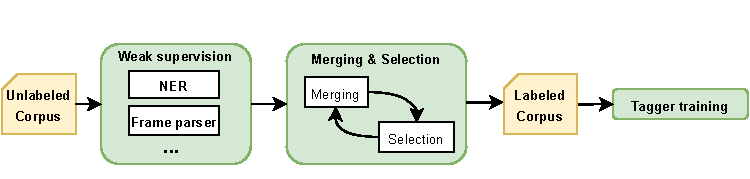
\includegraphics[width=0.9\textwidth]{images/weakly-supervised.pdf}
    \caption{Illustration of our pipeline. First, we analyze an unlabeled in-domain corpus with supplied domain-agnostic linguistic annotation models, such as a frame-semantic parser or NER. This results in slot candidates. Next, we iteratively merge and select slot candidates to obtain domain-relevant slots. Finally, we use the resulting slot labels in the corpus to train a neural slot tagger.}
    \label{fig:discover_overall}
\end{figure}
Figure \ref{fig:discover_overall} depicts a diagram describing our approach.
Our slot discovery method has three main stages:
\begin{enumerate}
    \item We obtain weak supervision labels from automatic generic annotation.
    We obtain this annotation using domain-independent natural language taggers such as a semantic frame parser or a named entity recognizer (NER).
    These models can detect important and relevant concepts in natural language utterances and subsequently group them using a set of pre-determined generic labels.
    Nevertheless, the raw output of these models is not polished and cannot be used for the purpose of the dialogue system directly.
    For more details, see Section~\ref{04:sec:tagging_concepts}.
    \item We identify domain-relevant slots based on the annotation labels by iteratively (a) merging and (b) ranking and selecting the most viable candidates (Section~\ref{04:sec:candidate_selection}).
    
    \item We use the discovered slots to train an independent slot tagger (Section~\ref{04:sec:training_tagger}).
\end{enumerate}

We refer to this approach as "weak supervision" because it uses noisy labels as input instead of the desired ones.

Consider an example in Figure \ref{fig:tagged_example}.
First, we note that it helps to use multiple tagging models since a respective model might not capture some of the concepts.
The set of tagged words from all the sources covers all the dialogue slot values (\emph{cheap}, \emph{Georgetown}).
However, it contains irrelevant words (\emph{restaurant}).
This behavior is expected since the tagging models are trained on generic open-domain data and detect all semantic concepts mentioned in the utterances.

Therefore, to exploit the output of generic models, we need to polish and customize it to the specific domain.
Our method combines multiple sources of semantic labels and selects only relevant slot candidates.
Slots discovered by our approach can then be used to design a schema relevant to a specific domain.
\begin{figure}[h]
\centering
    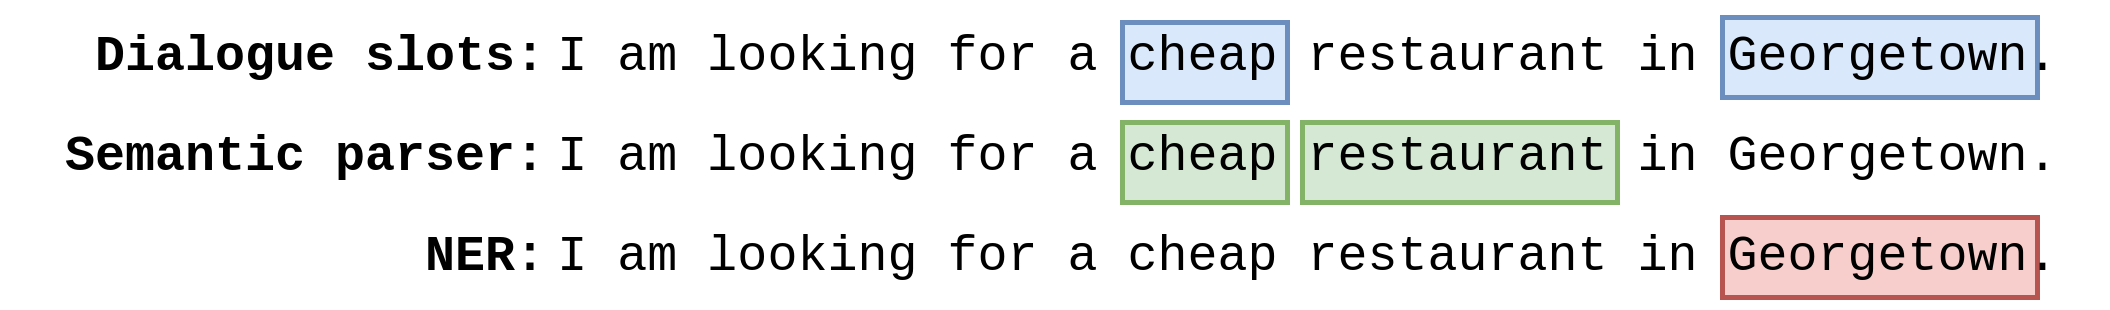
\includegraphics[width=0.8\textwidth]{images/tagging-example.png}
    \caption{An utterance from the restaurant recommendation domain tagged with generic semantic parser (green) and Named Entity Recognition system (red). We provide a comparison with ground truth dialogue slot labels (blue).}
    \label{fig:tagged_example}
\end{figure}

\section{Slot candidate identification by tagging semantic concepts}
\label{04:sec:tagging_concepts}

Our approach to selecting candidates for our method requires an initial pool of carefully chosen options representing coherent concepts. This step is critical to ensure the effectiveness of our selection process. We strive to gather as many candidates as possible to achieve this goal while preserving the above constraint.
One of the key features of our method is its ability to merge several concepts into one, which means that we aim for high granularity and specificity in our input labels. As a result, we need to ensure that each candidate represents a unique, distinguishable concept.

Given that we cannot rely on human annotations, we use an automatic procedure to gather the initial set of candidates.
This procedure combines multiple sequence tagging models to label the input corpus.
This procedure aims to identify words or phrases in the text representing distinct concepts that can be used as candidate labels.
We can use any sequence tagging NLP model that meets the following criteria: (1) a set of words with the same label indicates semantically coherent, distinct concepts, (2) no additional annotation is needed, and (3) the model is domain-independent.

For our experiments, we chose two types of taggers to obtain the input tags: Frame Semantic Parser and Named Entity Recognition (NER).
We can quickly and accurately identify candidate labels that meet our criteria by leveraging these models.


.
\begin{figure}[h!]
\centering
    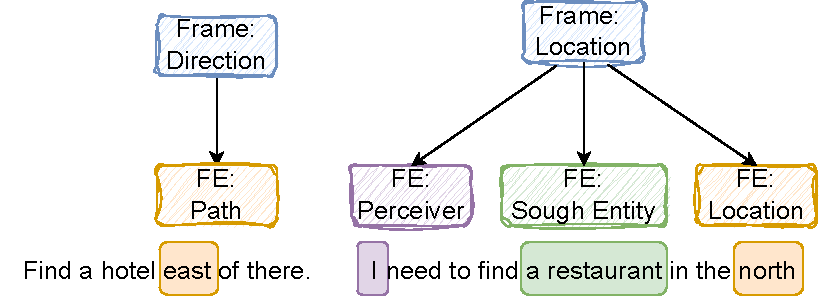
\includegraphics[width=0.8\textwidth]{images/framenet.pdf}
    \caption{An example of two Frames defined in the FrameNet dataset, together with core Frame Elements and respective instances. In this example, we can see that a semantic concept representing the location of some place can be captured by multiple frames (\emph{Direction} and \emph{Location}). However, from the perspective of dialogue systems, these differences are negligible. Therefore, we merge some of the candidates to obtain a simpler schema.}
    \label{fig:framenet}
\end{figure}

\paragraph{Frame Semantic Parser} The parser is based on the FrameNet project \cite{baker1998berkeley}.
FrameNet is a lexical database of the English language (although similar datasets exist in other languages) that aims to represent the usage of words in actual texts.
It contains over 200,000 utterances with over 1,200 frames, each representing one semantic concept.
From the NLP perspective, it can be approached as a task of Semantic Role Labeling.
Each frame is formed by one or more frame elements, which together form an instance of a certain semantic situation (e.g., \emph{Locale}, \emph{Offenses}, \emph{Size},...).
See Figure \ref{fig:framenet} for the example of FrameNet instances.
We take the individual Frame Elements as a source for our slot candidates.

\paragraph{Named Entity Recognition (NER)} is a well-established task of labeling occurrences of certain named entities in the input text data.
Typically, the NER labels \textit{word spans} that belong to a particular entity in the annotated utterance.
A common approach to identify the spans is BIO tagging \cite{ramshaw-marcus-1995-text}.
See the example in Table~\ref{04:tab:ner_example}.
\begin{table}[tp]
    \centering
    \begin{tabular}{c|c|c|c|c|c|c}
    \toprule
        \texttt{I} & \texttt{want} & \texttt{to} & \texttt{leave} & \texttt{from} & \texttt{{\color{cyan!80!yellow!80!black!100 }Edinburgh }} & \texttt{{\color{cyan!80!yellow!80!black!100 }Waverley}}. \\
        \textbf{O} & \textbf{O} & \textbf{O} & \textbf{O} & \textbf{O} & \textbf{B} & \textbf{I}\\
    \bottomrule
    \end{tabular}
    \caption{An example of BIO tagging to identify named entities.}
    \label{04:tab:ner_example}
\end{table}
It fits our requirements well because the task is universal, and the named entities definition is not specific to any particular domain.

\section{Unsupervised candidate identification}
\label{04:sec:unsup_candidate_selection}
The approach introduced in this chapter is limited by the requirement of third-party models to gather the initial set of candidates.
Therefore, we experiment with alternative ways of obtaining slot candidates completely unsupervised.
This can lift the requirement of using generic models fine-tuned on out-of-distribution data.

\subsection{Memory Networks for candidates identification}
\label{04:sec:memnn}
The end-to-end Memory Networks architecture described in Chapter~\ref{02:sec:mem_nn} suits our needs for an unsupervised slot candidate identification.
We train the Mem2Seq (see Sec.~\ref{02:sec:mem2seq}) model on the target dataset to learn the copy behavior.
We then use the trained model to obtain a set of slot candidates.
To achieve this, we let the model generate the test dialogues individually and inspect its behavior.

The Mem2Seq model's knowledge base entries represent entities or their properties, such as addresses.
Furthermore, the model saves the conversation context via the memory mechanism.
The content of the memory is further used to copy its entries directly to the produced response.
Specifically, during the response generation process, the model decides whether the new token will be generated from decoder vocabulary distribution or copied from memory.
The intuition is that when a certain token should appear in the generated response, the model decides to copy it rather than generate it to prevent mistakes.
We save each token that is copied into the produced response rather than generated.
These tokens will likely be slot candidates as they supposedly correspond to entities and slot values mentioned in the context.
We then run k-means clustering to obtain a set of slot candidates.
This way, we obtain multiple groups of word forms that can be used as input for our slot discovery pipeline.

We also note the similarity of this approach to the two-step generation process used in multiple architectures~\citep{lei2018sequicity, peng2021soloist}.
In the first step of this process, the model generates placeholders such as \emph{[address]} instead of specific values.
This delexicalized utterance is then lexicalized in the second step by replacing the placeholders with actual values, e.g. using the database.
This is almost exactly what happens in the Mem2Seq model.
Only the two steps are joined in one, so the model puts the database values indirectly.
Also, the lexicalization procedure of placing values instead of placeholders is learned rather than hardcoded.

\subsection{LLMs for candidate identification}
\begin{table}[tp]
    \centering
    \begin{tabular}{r|l}
    \toprule
        \textbf{Prompt} & \texttt{{\color{cyan!80!yellow!80!black!100 }Extract important concepts or objects }}\\
        & \texttt{{\color{cyan!80!yellow!80!black!100 }from the following utterance. }} \\
        & \texttt{{\color{cyan!80!yellow!80!black!100 } Yield all the concepts in one-level JSON dictionary. }} \\
        & \texttt{{\color{cyan!80!yellow!80!black!100 } Include only entities and concepts that}} \\
        & \texttt{{\color{cyan!80!yellow!80!black!100 } are mentioned in the utterance.}} \\
        & \texttt{{\color{cyan!80!yellow!80!black!100 } Don't provide the intent.}} \\
        & \texttt{{\color{cyan!80!yellow!80!black!100 } See the following examples:}} \\
        & \texttt{{\color{orange!50!yellow!90!black!100!} ---------- Example ------}} \\
        & \texttt{{\color{orange!50!yellow!90!black!100!} Utterance: "I am looking for a theater }} \\
        & \texttt{{\color{orange!50!yellow!90!black!100!} that is reasonably priced." }} \\
        & \texttt{{\color{orange!50!yellow!90!black!100!} Output: \{'venue': 'theater', 'price': 'reasonable'\} }} \\
        & \texttt{{\color{orange!50!yellow!90!black!100!} -------------------------}} \\
        & \texttt{{\color{cyan!80!yellow!80!black!100 } Now complete the following example: }} \\
        & \texttt{{\color{cyan!80!yellow!80!black!100 } Utterance:}  {\color{red!100!yellow!90!black!100!}"I am looking for a cheap hotel."}} \\
        & \texttt{{\color{cyan!80!yellow!80!black!100 } Output:  }} \\
        \bottomrule
    \end{tabular}
    \caption{The {\color{cyan!80!yellow!80!black!100 }prompt}, which is used to obtain slot candidates from the input utterance. It contains an {\color{orange!50!yellow!90!black!100!} example} to specify the desired output structure }
    \label{04:tab:prompt}
\end{table}

Another way of obtaining the slot candidates is by employing Large Language Models.
These models can be instructed in the input text (prompted) to perform virtually any task (see Section~\ref{background:plms}).
In our case, we instruct the model to extract the potential slot candidates directly from the input utterance.
We use two models: \emph{Tk-Instruct-11B} \cite{supernaturalinstructions}, which is T5 encoder-decoder architecture \cite{2020t5} tuned on a dataset of over 5M task instances with instructions and \emph{ChatGPT} which is a closed source product introduced by the OpenAI company\footnote{\url{https://openai.com/blog/chatgpt}}.
The used prompt is given in Table~\ref{04:tab:prompt}.
We use both models in parallel to obtain two sets of candidates.
We then use a clustering procedure similar to the process described in~\ref{04:sec:memnn}.
Note that although the model categorizes the extracted words as part of the output, the category names are arbitrary and inconsistent among examples.
For example, the model can categorize a word \emph{Italian} once as \textit{food\_type} and on another occasion as \emph{nationality}.
Therefore, we do not use them to obtain the slot groups directly.
This leaves us with a set of slot candidates again used as input to our pipelined method.

\section{Selection of slot candidates}
\label{04:sec:candidate_selection}
% \begin{figure}[ht]
%     \centering
%     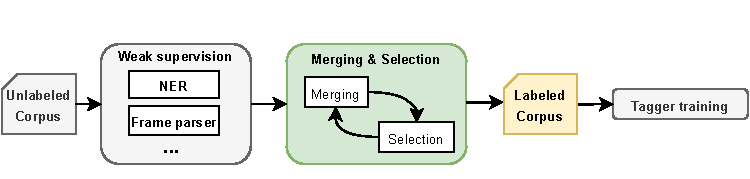
\includegraphics[width=0.9\textwidth]{images/merging.pdf}
%     \caption{The selection step in our pipeline processes the input data and yields a set of slot candidates that should be relevant to the target domain.}
%     \label{fig:candidate_selection}
% \end{figure}
In the previous step, we obtained a superset of all the slot candidates using weak supervision from the tagging models.
Subsequently, we need to identify domain-relevant slots based on candidates provided by the automatic annotation.
To achieve this, we design an iterative slot discovery procedure -- in each iteration, we: 
(1) merge similar candidates, 
(2) rank candidates' relevance and eliminate irrelevant ones.
Once no more frames are eliminated, the process stops and we obtain slot labels, which are used to train a slot tagger (see Section~\ref{04:sec:training_tagger}).

We refer to the automatically tagged tokens as \emph{(slot) fillers}, and the tags are considered slot candidates.
To be able to select relevant candidates, we need to represent them in continuous space.
We use word embedding vectors and compute \emph{slot embeddings} $e(s_k)$ for each 
distinct slot candidate $s_k$ as word embedding averages over all respective slot fillers, weighted proportionally by filler frequency.
The merging step requires the slot embeddings to be re-computed after each iteration.
We will now describe the individual steps.

\subsection{Candidate Merging}
\label{03:candidate_merging}
Since automatic annotation may have a very fine granularity, multiple slot candidates often capture entities/objects of the same type.
This is the case for frame-semantic annotation, which we mostly use in our experiments.
With a frame parser, for instance, the frames \emph{Direction} and \emph{Location} both relate to the concept of \emph{area}, which can be represented as a single slot.
Thus, we must merge similar slot candidates subsets $s_1 \dots s_n$ under a single candidate.
We further use a syntactic parser to obtain dependency relations in which the slot fillers appear in the data and use this information to get more accurate similarity scores.
We measure the similarity of slot candidates $s_1,s_2$ as:
\begin{equation}
    \text{sim}(s_1,s_2) = \text{sim}_{e}(e(s_1),e(s_2)) + \text{sim}_{\text{ctx}}(s_1,s_2)
\end{equation}
where $\text{sim}_{e}$ is a cosine similarity and $\text{sim}_{\text{ctx}}(s_1,s_2)$ is a normalized number of occurrences of $s_1$ and $s_2$ with the same dependency relation.
If the similarity exceeds a pre-set threshold $T_{\text{sim}}$, the candidates are merged into one.

\subsection{Candidate Ranking and Selection}
\label{04:candidate_select}
In this step, we aim to eliminate irrelevant slot candidates and exclude them from the selection process.
To achieve this, we rank the slot candidates with respect to their importance computed from the data.
We hypothesize that different slots are likely to occur in different contexts (e.g., addresses are mentioned more when the system provides information to the user rather than stated by the user).
Some slots can occur rarely but still be relevant.
However, such rare slots would be overshadowed by more frequent slot candidates.
To preserve relevant slots that only occur in rarer contexts, we cluster the data into multiple clusters and then rank the candidates within each cluster separately.
Finally, we filter the candidates according to a threshold.
Specifically, we consider all candidates with a score higher than the chosen threshold relevant and select them for the next iterations.
The threshold is determined as an $\alpha$-fraction of a given cluster mean where $\alpha$ is chosen empirically.
If a slot candidate is selected in at least one of the clusters, it is considered viable overall.

\paragraph{Clustering the data}
The data clustering step aims to distinguish contexts in which the candidates appear.
We simplify the notion of context to the head verb connected with the respective slot filler word.
We process the data with a generic semantic role labeling tagger to obtain verb dependency relations.
Each occurrence of a filler is thus associated with a \emph{head verb} whose semantic argument the corresponding word is, if such exists. 
To give an example, consider \emph{verb-filler} pairs such as \emph{want-chinese} or \emph{reserve-hotel}.
We then compute embeddings of the formed pairs.
To do this, we take an embedding of both the head verb and the fillers and average them.
The pairs are then clustered using agglomerative (bottom-up) hierarchical clustering with average linkage according to the cosine distance of their embeddings.
Note that fillers for the same slot candidate may end up in multiple clusters.
This does not mean that the respective slot candidate is split -- it is just ranked for relevance multiple times (with respect to multiple contexts).
The process stops when a predetermined number of clusters is reached.

\paragraph{Candidate Ranking criteria}
We need a function that computes a score for each candidate to rank the candidates.
Since it is unclear how to compute the score, we combine multiple attributes to compute the final score.
Specifically, we compute the following characteristics for each candidate:
\begin{itemize}
    \item \textbf{Frequency} $\text{frq}(s)$ is used since candidates that occur frequently in the data are likely important.
    
    \item \textbf{Coherence} $\text{coh}(s)$ is the average pairwise similarity of all fillers' embeddings:
    \begin{equation}
        \text{coh}(s) = \frac{\mathlarger{\sum}_{(v,w) \in C^2_s}{d_{\cos}(e(v), e(w))}}{|C^2_s|}
    \end{equation}
    where $C^2_s$ is a set of all pairs of fillers for the slot candidate \emph{s}.
    We follow \citet{chen2014leveraging}'s assumption that fillers with high coherence, i.e., focused on one topic, are good slot candidates.
    
    \item \textbf{TextRank} \cite{mihalcea2004textrank} is a keyword extraction algorithm similar to the well-known PageRank~\citep{page1999pagerank}.
    It constructs a graph where nodes represent words and edges represent their co-occurrence.
    The dominant eigenvector of the adjacency matrix of this graph then gives the individual words' scores.
\end{itemize}
The final score is a simple sum of rankings with respect to all three scores.
For TextRank and frequency, we use a placeholder representing the slot candidate instead of the respective fillers.
Therefore, we obtain scores relevant to candidates rather than the individual words.

\section{Training standalone tagger}
\label{04:sec:training_tagger}
% \begin{figure}[h]
%     \centering
%     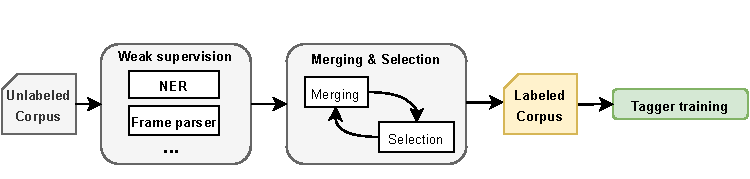
\includegraphics[width=0.9\textwidth]{images/tagging.pdf}
%     \caption{After the set of slots is selected we assign the obtained labels to their occurrences in the data and use this labeled corpus to train a standalone tagger. }
%     \label{fig:training_tagger}
% \end{figure}
The steps described in Sections~\ref{04:sec:tagging_concepts}, \ref{04:sec:unsup_candidate_selection} and \ref{04:sec:candidate_selection} can give us a good set of dialogue slots. % to be tracked.
However, directly using the merged and filtered slots may result in low recall since the original annotation models used as weak supervision are not adapted to our specific domain.
Therefore, we use the obtained labels to train a new, domain-specific slot tagger to improve performance.
The tagger has no access to better labels than those derived by our method; however, it has a simpler task, as the set of target labels is now much smaller, and the domain is much narrower.

The motivation for training a tagger is two-fold.
First, its usage makes it possible to discard a dependency on the candidate identification models in runtime.
Thus, the method is simpler to apply. 
Second, although the selection process can yield a good set of slot candidates, we experimentally discovered that the quality of the taggers used for initial input labeling can be insufficient, especially for some domains.
Therefore, directly using the merged and filtered slots may result in low recall since the original annotation models used as weak supervision are not adapted to our specific domain.

We model the slot tagging task as sequence tagging, using a convolutional neural network that takes word- and character-based embeddings of the tokens as the input and produces a sequence of respective tags \cite{lample2016neural}.\footnote{\url{https://github.com/deepmipt/ner}}
The output layer of the tagger network gives softmax probability distributions over possible tags.

\paragraph{Increasing recall} To further increase recall, we add an inference-time rule -- if the most probable predicted tag is `O' (i.e., no slot) and the second most probable tag has a probability higher than a preset threshold $T_{\text{tag}}$, the second tag is chosen as a prediction instead.
As we discuss in Section \ref{04:sec:discovery_results}, this threshold is crucial for achieving substantial recall improvement.

\paragraph{Tagging model robustness} 
We only use 10\% of the original in-domain training set (with labels from Section~\ref{04:sec:tagging_concepts}) to train the slot tagger model.
The rest of the training set is used for a grid search to determine model hyperparameters (hidden layer size, dropout rate, and $T_{\text{tag}}$ threshold). We choose the parameters that yield the best F1 score when compared against the automatic slot discovery results (i.e., no manual annotation is needed here; the aim is a good generalization and improved robustness of the resulting model).


\section{Experimental setup}
\label{04:sec:discovery_results}
In this section, we provide a quantitative analysis of the results with respect to the NLU performance and quality of the discovered slots.
We also evaluate the application of this method as a module in the end-to-end dialogue system model.
\paragraph{Datasets}
We use multiple datasets to evaluate the proposed method extensively and gain more insights.
The datasets vary in several properties, like domain count or collection process.
This means we can compare the results on different data distributions and tasks with different complexities.
For more detailed dataset descriptions, please refer to Section \ref{02:sec:input-data-desc}.
Here, we provide only a concise list with basic descriptions.
\begin{itemize}
    \item \textbf{CamRest676} (\textbf{CR}) is dataset of 2,744 user utterances, all in the restaurant reservation domain.
    \item \textbf{Cambridge SLU} (\textbf{CS}) is in the same domain as CamRest676 but only focuses on NLU annotation of  10,569 user utterances.
    \item \textbf{MultiWOZ} is a multi-domain dialogue corpus. For experiments in this chapter, we picked only single-domain dialogues from two domains -- hotel reservation and attraction recommendation -- to form \textbf{WOZ-hotel} (\textbf{WH}) with 14,435 utterances, 9 slots, 3 intents and \textbf{WOZ-attr} (\textbf{WA}) with 7524 utterances, 8 slots and 3 intents respectively.
    \item \textbf{ATIS} (\textbf{AT}) is focused on flight search and contains nearly 5,000 utterances.
\end{itemize}
\paragraph{3rd party models}
As sources of weak supervision providing slot candidates, we mainly use the frame semantic parsers \textit{SEMAFOR} \cite{das2010semafor} and \textit{open-sesame} \cite{swayamdipta2017frame} -- a union of labels provided by both parsers is used in all our setups. In addition, to explore combined sources on the named-entity-heavy ATIS dataset, we include a generic convolutional NER model provided by SpaCy.\footnote{\url{https://spacy.io}}
To provide features for slot candidate merging and selection, we use AllenNLP \cite{Gardner2017AllenNLP} for SRL
and FastText \cite{bojanowski2017enriching} as pre-trained word embeddings.

\subsection{Training details}
\begin{itemize}
    \item Slot merging and selection parameters were set heuristically in an initial trial run on the CamRest676 data and proved stable across domains.
    \item Slot tagger hyperparameters are chosen according to grid search on a portion of the training data.
    \item Since the models are rather small concerning the number of parameters, it is sufficient to use a regular desktop PC. In our experiments, we require about 4 GB of RAM and use Intel Xeon E5-2630 v4 CPUs. 
    \item Our slot candidate selection step takes roughly 1 hour.
    The tagger model is lightweight, with only 150k parameters. Its training requires 10-30 minutes, depending on the exact configuration and data size.
    \item We conduct a hyperparameter search using a basic grid search algorithm. We tested hidden size values $\in [50,200]$, dropout $\in [0.5,0.85]$ and the threshold $T_{\text{tag}} \in [0.05,0.3]$. Therefore, we ran $4\times8\times6 = 192$ search trials.
    \item The best parameters were determined by tagger accuracy on the validation set: hidden\_size = 250, dropout = 0.7, $T_{\text{tag}} = 0.3$, $T_{\text{sim}} = 0.9$.
    \item For data without explicit \emph{train:validation:test} splits we use ratio of sizes \emph{8:1:1}.
\end{itemize}

\subsection{Evaluated systems}
We test multiple variants of our system.
This gives us an idea about the contributions of all the individual methods we propose.
Here we give an overview of all the system variants:
\begin{itemize}[nosep,leftmargin=10pt]
    \item \textit{Ours-full} is the full version of our method (full annotation setup and trained slot tagger).
    \item \textit{Ours-nothr} does not use the recall-increasing second-candidate rule in the slot tagger.
    \item \textit{Ours-notag} excludes the slot tagger. This means that the outputs of input taggers are used directly to annotate the data.
    \item \textit{Ours-nocl} further excludes the clustering step; slot candidate ranking and selection is performed over all candidates together.
\end{itemize}
We also compare to previous work of \citet{chen2014leveraging}\footnote{We use our re-implementation of their approach.}.
This method is similar to the variant \textit{Ours-nocl} but does not merge similar frames and uses different ranking criteria.
Essentially, they use the outputs of the input tagger directly after the selection step without further processing.

To put our results into perspective, we also include two supervised models for comparison:
\emph{Tag-supervised} is the same model that we use as our slot tagger (see \ref{04:sec:training_tagger}), but it is trained on supervised data with all ground truth labels available.
The other supervised baseline is called \emph{Dict-supervised}.
It uses a simple dictionary of slot fillers obtained directly from the training data.
We use straightforward word matching based on regular expressions to tag occurrences of these values.

Apart from evaluating the tagging performance with respect to NLU, we are also interested in the intrinsic evaluation of the verb-slot pair clusters formed for slot ranking.
Specifically, we ask how well these clusters are formed and if they are meaningful.
We compare to gold-standard intent annotation with respect to the following baselines: (1) a majority baseline (assigning the most frequent intent class to all instances), and (2) a simple method that represents the utterances as averages of respective word embeddings and performs sentence-level intent clustering.
All the slots in a given utterance are assumed to have the same intent.

\section{Evaluation}
We need a way of comparing the predicted structure to the ground truth to evaluate the discovered set of slots.
Therefore, we construct a handcrafted mapping between our discovered slots and the respective ground-truth slots.
Importantly, this mapping is only needed for evaluation; \textbf{our method does not depend on it}.
The mapping is domain-specific, but it is very easy to construct even for an untrained person -- the process takes less than 10 minutes for each of our domains.
It amounts to matching slots from the domain ontology against slots output by our approach, represented by the FrameNet labels.
We provide an example of such a reference mapping in Table \ref{03:ref_mapping}.
\label{sec:app-ref-mapping}

\begin{table}[tp]
    \centering
    \small
    \begin{tabular}{rcl}
    \textbf{\emph{Ours-full} output} & & \textbf{CambridgeSLU ontology}\\\hline
     Expensiveness & $ \mapsto$ & Pricerange\\
     Origin + People\_by\_origin & $ \mapsto$ & Food\\
     Direction + Part\_orientational & $ \mapsto$ & Area\\
     Contacting + Artifact & $ \mapsto$ & Phone\\
     Locale\_by\_use & $ \mapsto$ & Type \\
     

    \end{tabular}
    \caption{An example of reference mapping between the output of \emph{Ours-full} represented by FrameNet labels (left) and ground-truth CambridgeSLU ontology (right).
    Frames merged by our method are shown on a single line, separated by “+”.
    }
    \label{03:ref_mapping}
\end{table}

We use some common metrics described in Section \ref{02:sec:eval_metrics} for quantitative evaluation.
Specifically we use \textbf{Intent Accuracy}, \textbf{Joint Goal Accuracy} and \textbf{Entity Match Rate.}
We also use some metrics specific to this part of the work:
\begin{itemize}
    \item \textbf{Slot F1 score}: To reflect slot tagging performance, we measure precision, recall, and F1 for every slot individually.
    An average is then computed from slot-level scores, weighted by the number of slot occurrences in the data.
    We measure slot F1 on standalone user utterances (slot tagging) and in the context of a dialogue system (dialogue tracking).
    \item \textbf{Slot-level Average Precision (AP)}. The slot candidates picking task is a ranking problem, and we use the \textit{average precision} metric following \citet{chen2014leveraging}.
    Considering a ranked list of discovered slots $l = s_1, \dots, s_k, \dots, s_n$ we compute AP:
    \begin{equation}
        AP(l) = \frac{\sum_{k=1}^n P@k(l)\mathbbm{1}_k}{\mbox{\#\,mapped\ slots}}
    \end{equation}
    where $\mathbbm{1}_k$ is an indicator function that equals one if slot $k$ has a reference mapping defined and $P@k(l)$ is precision at $k$ of the ranked list $l$.
    \item \textbf{Slot Rand Index (RI)} is a clustering metric used to evaluate slot candidate merging. RI is the proportion of pairs of slot candidates correctly assigned to the same or different slots (following the reference mapping).\footnote{We compute RI on a union of labels with a ground-truth slot mapping and all labels selected by our method. Labels without ground-truth mapping are assumed to form single-item “pseudo-slots”.}
    
    \item \textbf{Normalized Mutual Information (NMI)} is the mutual information between two clusterings normalized into the (0, 1) interval.
    Thanks to the normalization, it is suitable for comparing two clusterings with different numbers of clusters.
\end{itemize}

For slot tagging and ranking evaluation, we sampled a random data order 50 times and performed 5-fold cross-validation for each permutation.
For the dialogue generation evaluation, we trained the models 100 times and used averaged results.
All results are given with 95\% confidence intervals.

\begin{figure}[h]
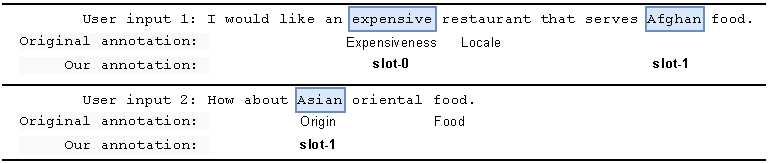
\includegraphics[width=1.0\textwidth]{images/label_example.pdf}
%\newtcbox{\bluebox}[1][]{nobeforeafter, tcbox raise base, shrink tight, sharp corners, extrude by=1mm, colback=blue!15, colframe=blue, #1}
%\newtcbox{\graybox}[1][]{nobeforeafter, tcbox raise base, shrink tight, sharp corners, extrude by=1mm, colback=gray!15, colframe=gray, #1}
%\small
%        \centering
%        \begin{tabular}{rl}
%        \hline
%        \texttt{user input 1:} & \textit{\texttt{I would like an \bluebox{expensive} \graybox{restaurant} that serves \bluebox{Afghan} food }} \\
%        \texttt{original annotation:} & \hspace{29mm} Expensiveness \hspace{4mm} Locale \hspace{33mm} - \\
        %\rowcolor{lightblue}
%        \texttt{our slot tagger:} & \bf\hspace{31mm} slot-0 \hspace{15mm} - \hspace{38mm}slot-1  \\
%        \hline
%        \texttt{user input 2:} & \textit{\texttt{How about \bluebox{Asian} oriental \graybox{food}?}} \\
%        \texttt{original annotation:} & \hspace{19mm} Origin \hspace{19mm} Food \\
        %\rowcolor{lightblue}
%        \texttt{our slot tagger:} & \bf\hspace{20mm}slot-0 \hspace{22mm} - \\
%        \hline
%        & ...
%        \end{tabular}
        \caption{A sample of a dialogue from CamRest676 data, with labels from a frame-semantic parser (middle) and our slot tagger (bottom).
        Although ``Afghan'' food is not in the frame parser output, our tagger could recognize it. The second utterance successfully captures the change in value for slot-1 (corresponding to food type). This shows that our model can categorize entities (both ``Afghan'' and ``Asian'' relate to the same slot).}
    \label{fig:example}
\end{figure}

\begin{figure}
    \centering
    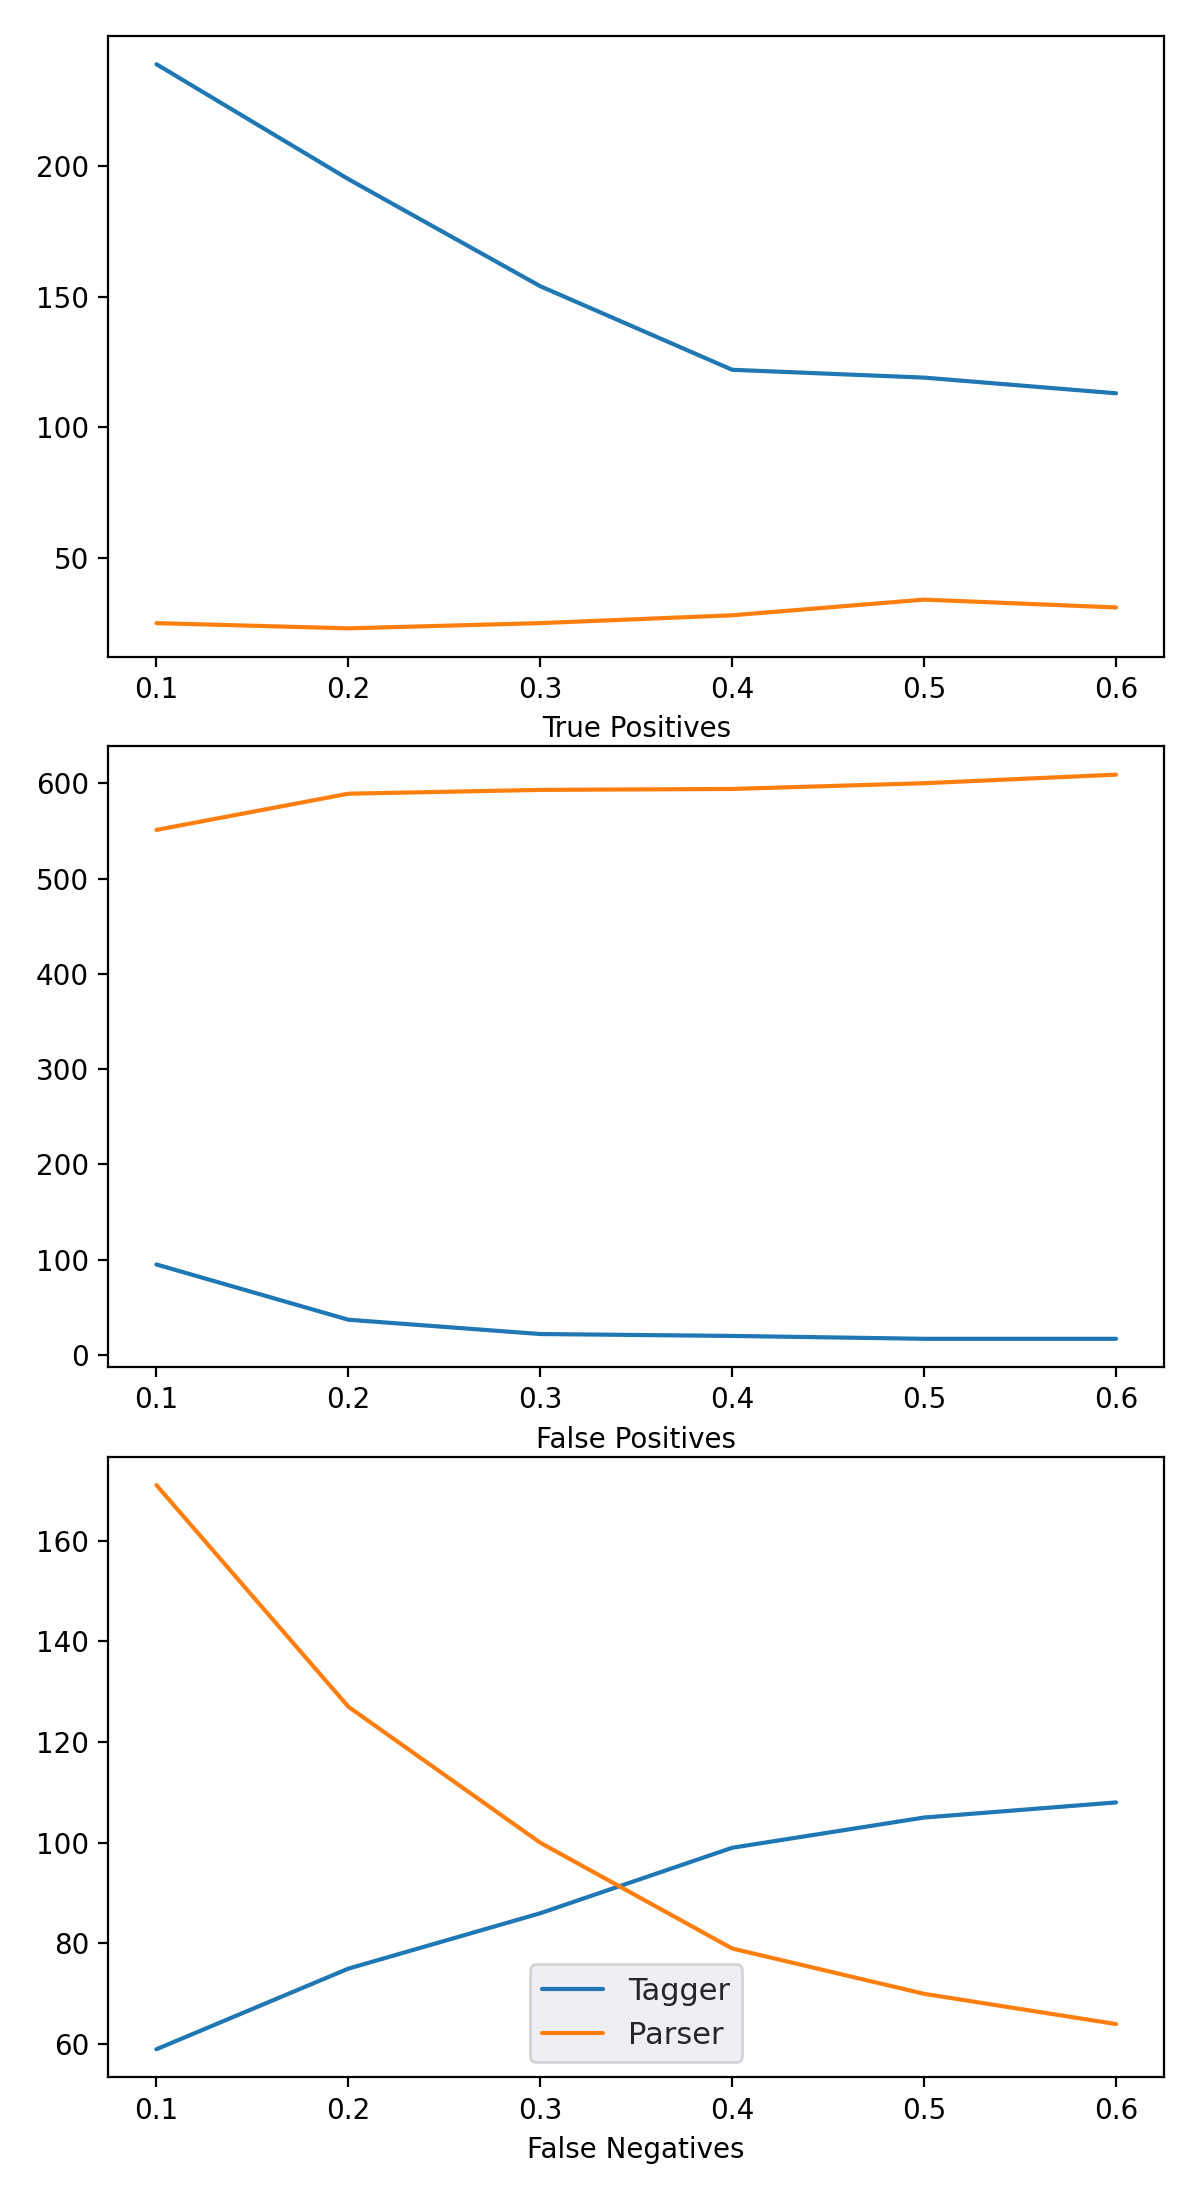
\includegraphics[width=0.6\textwidth]{images/slots.png}
    \caption{The comparison of outputs of our tagger and the parser. The plots show a number of cases in which the respective approach encounters more TPs, FPs, or FNs than the other.}
    \label{fig:tagger_comp}
\end{figure}

\section{Results}
We evaluate our approach to slot discovery by comparing the resulting slot labels to gold-standard supervised slot annotation.

\paragraph{Slot tagging}\hspace{-3mm} is evaluated in Table \ref{table:slotfilling}.
\emph{Ours-full} (slot selection + trained tagger) outperforms all other approaches by a large margin, especially regarding recall.

The performance cannot match the supervised models, but it is not far off in some domains.\footnote{Note that our measurements of slot F1 only consider the `O' tag as negative (the average is computed over slots only). This results in lower numbers than those reported in literature \cite{goo_slot-gated_2018}, but we believe this reflects the actual performance more accurately.}
\citet{chen2014leveraging}'s method has a slightly higher precision, but our recall is much higher than theirs.
Note that \citet{chen2014leveraging} do not reduce the set of candidates.
They only rank them so that a manual cut-off can be made.
In contrast, our method reduces the set of candidates significantly.
A comparison between \textit{Ours-notag} and \textit{Ours-full} shows that applying the slot tagger improves both precision and recall.
Tagger without the threshold decision rule (\textit{Ours-nothr}) mostly performs better than the parser; however, using the threshold is essential to improve recall.
Experiments on ATIS with NER as an additional annotation source proved that our method can benefit from it.
As discussed above, using the trained tagging model is crucial to improve the recall of our method. In Figure~\ref{fig:tagger_comp}, we compare the results with and without the tagger. We change the value of the prediction threshold and measure the number of cases in which the tagging model encounters more true positives, false positives, or false negatives, respectively. As the results show, lowering the threshold increases the number of cases in which the tagger finds more correct slot values (and therefore improves recall), while it does not affect the number of false positives much (and therefore retains precision).
\begin{table}[tp]
        \centering
        \small
        \begin{tabular}{l|c|c|c|c}
        \hline
         \textbf{method} $\downarrow$ / \textbf{dataset}$ \rightarrow$ &  \textbf{CS} & \textbf{WH} & \textbf{WA} & \textbf{AT} \\
         \hline
        Tag-supervised$^\ast$ & $0.724 \pm .003 $ & $\pmb{0.742} \pm .008$ & $\pmb{0.731} \pm .002$ & $\pmb{0.848} \pm .003$ \\
         Dict-supervised$^\ast$ & $\pmb{0.753} \pm .005 $ & $\pmb{0.750} \pm .018$ & $0.665 \pm .003$ & $0.678 \pm .002$ \\\hline
        \bf weak supervision $\rightarrow$ & frames & frames & frames &  frames,NER \\\hline
         Chen et al. & $0.590 \pm .001 $ & $0.382 \pm .001$ & $0.375 \pm .001$ & $0.616 \pm .001$  \\\hdashline[0.5pt/2pt]
         %\hline
         Ours-nocl & $0.393 \pm .011 $ & $0.122 \pm .001$ & $0.266 \pm .008 $ & $ 0.677 \pm .002$ \\
         %\hline
         Ours-notag & $0.664 \pm .007$ & $0.388 \pm .002$ & $0.383 \pm .002$ & $ 0.648 \pm .003$ \\
         Ours-nothr & $0.569 \pm .031$ & $0.485 \pm .032$ & $0.435 \pm .002 $ & $0.698 \pm .004$\\
         %\hline
         Ours-full & $\pmb{0.692} \pm .008$ & $\pmb{0.548} \pm .004$ & $\pmb{0.439} \pm .001$ & $\pmb{0.710} \pm .002$ \\
         \hline
        \end{tabular}
                 
        \caption{F1 score values with 95\% confidence intervals for slot tagging performance comparison among different methods. The measures are evaluated using a manual slot mapping to the datasets' annotation, which is unnecessary for the methods. $^\ast$Note that supervised setups are not directly comparable to our approach.
        \label{table:slotfilling}
        }
\end{table}

\paragraph{Performance of unsupervised candidate identification}
We separately evaluate the setup in which we used unsupervised sources of candidate identification described in Section~\ref{04:sec:unsup_candidate_selection}.
In Table~\ref{04:tab:unsup-discovery}, we present the performance of the overall pipeline for various candidate identification methods with and without applying our full pipeline (see~\ref{04:sec:overview}).
We can see that applying our pipeline improves the performance, especially the overall recall.
We also compare the pipeline performance with various candidate identification methods in Figure~\ref{04:fig:compare_sources}.
This comparison shows that the FrameNet-based candidate identification mechanism outperforms unsupervised variants.
\begin{figure}[h]
    \centering
    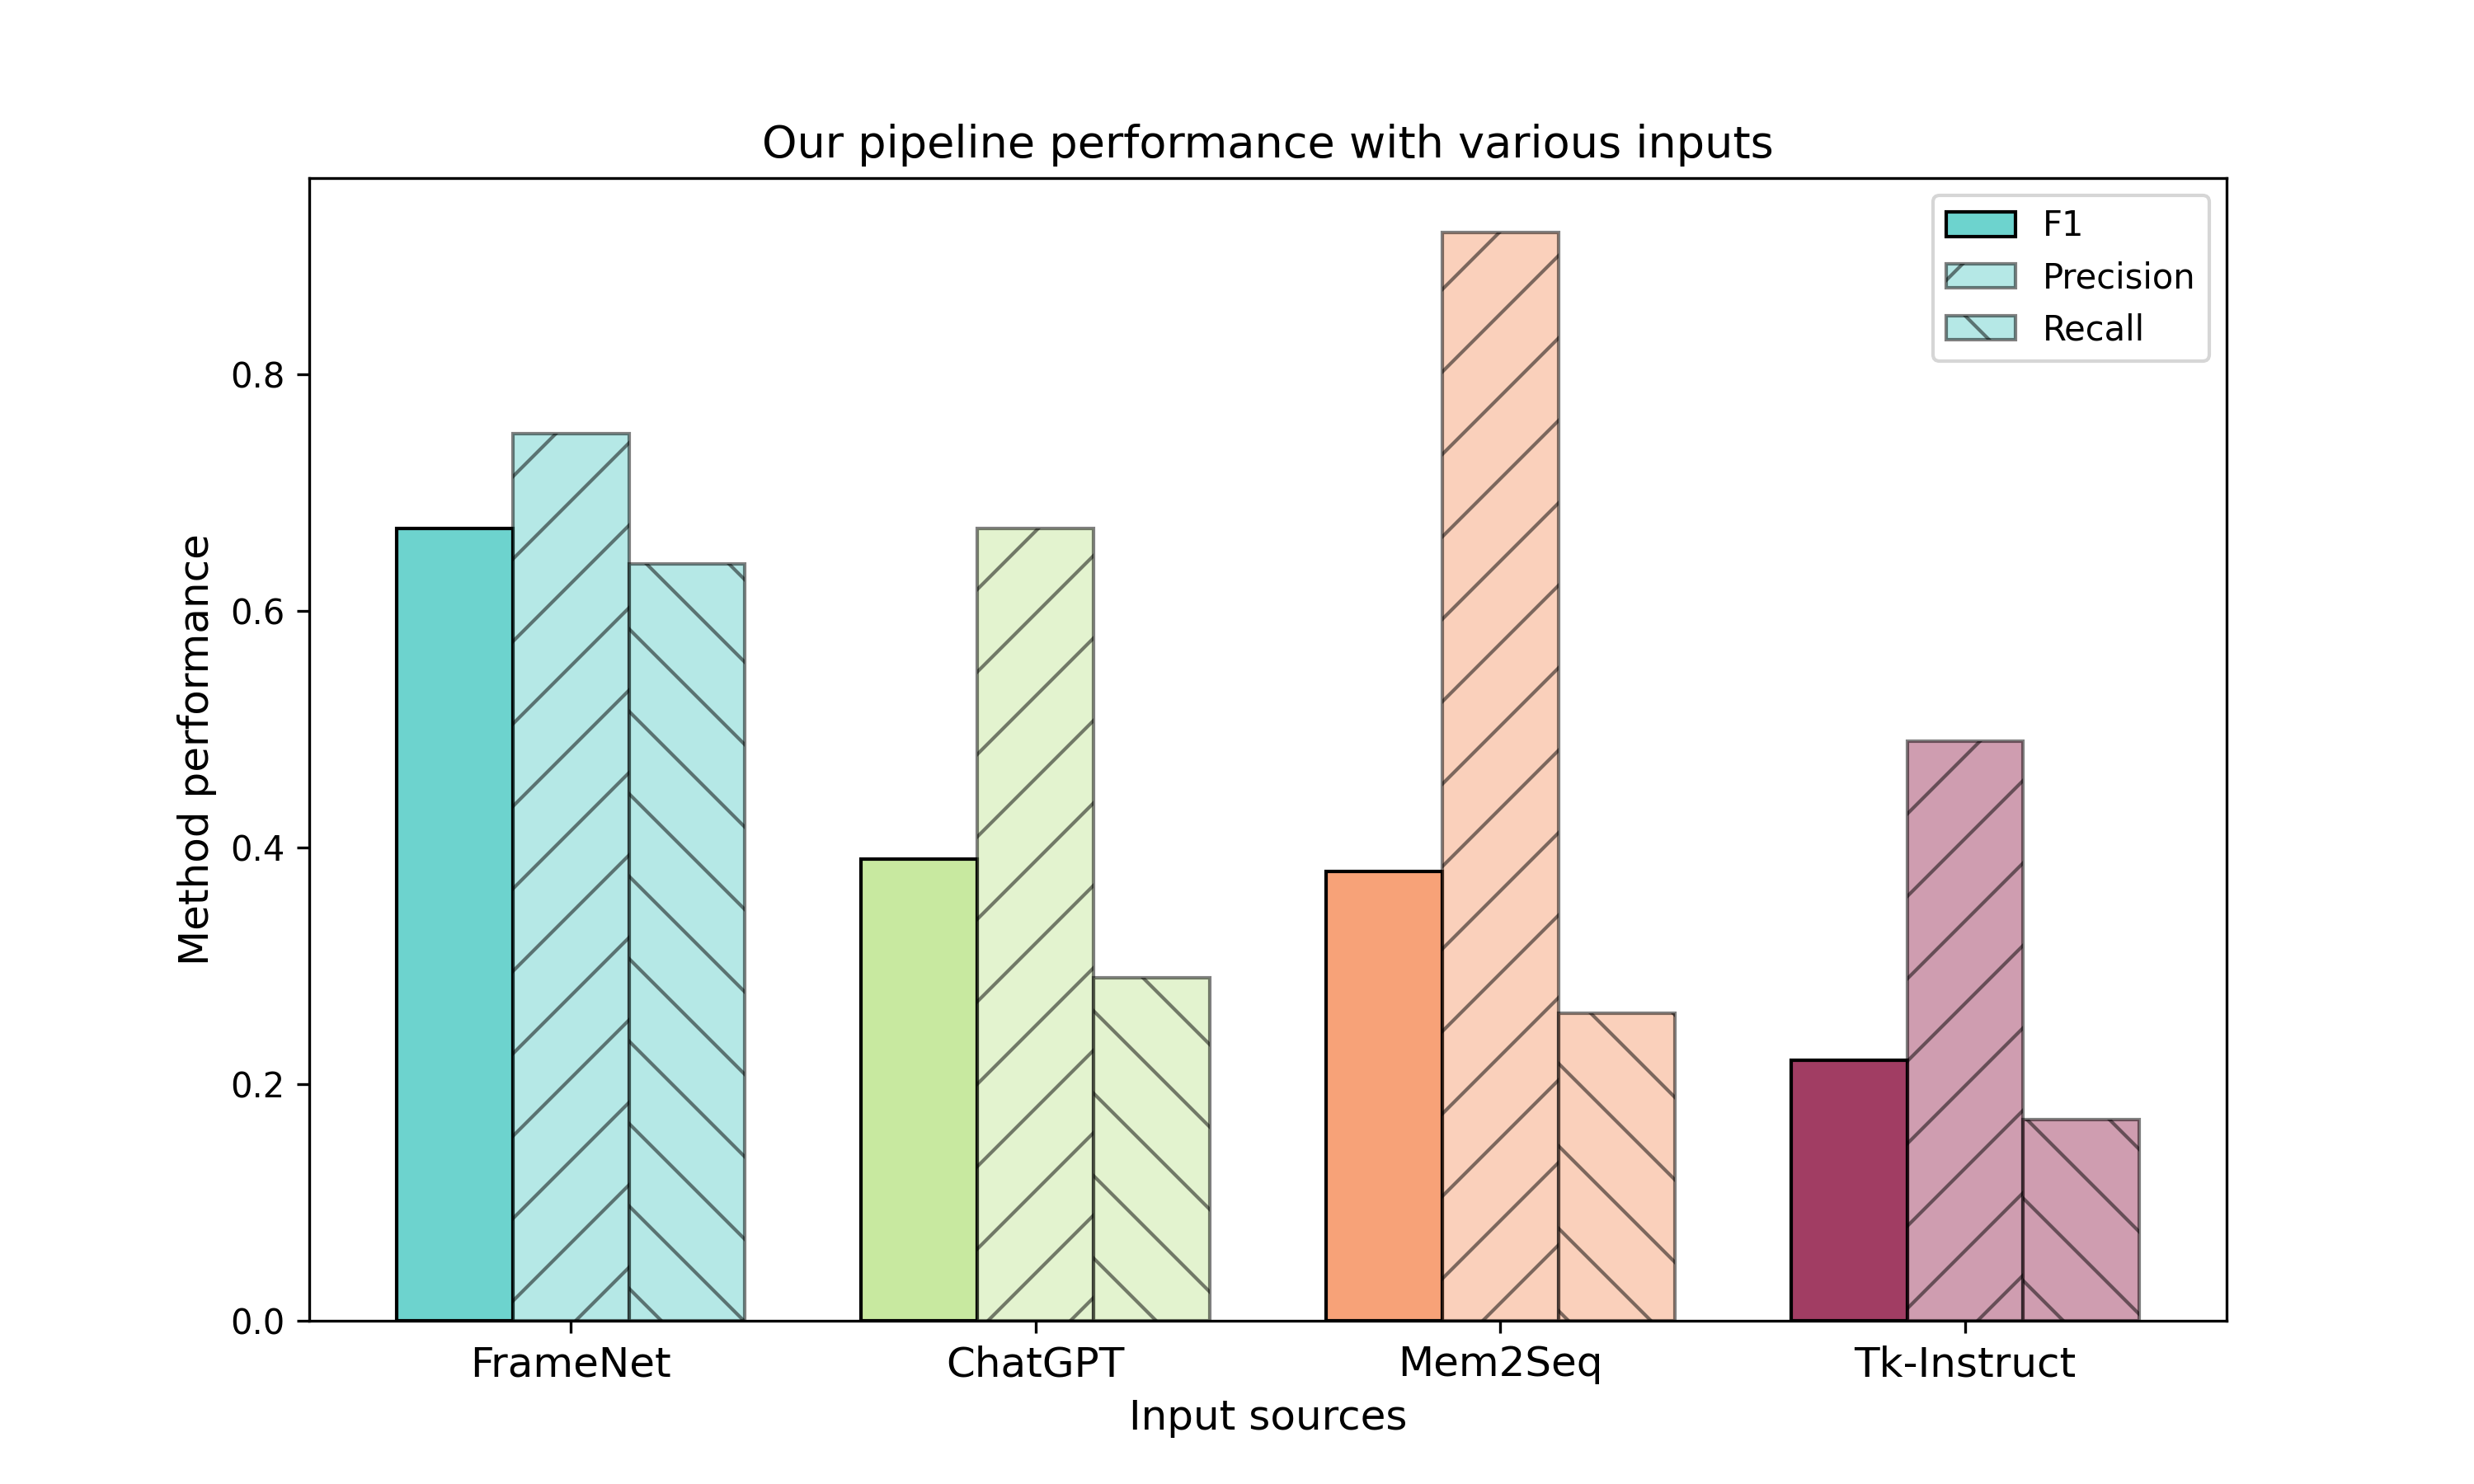
\includegraphics[width=0.9\textwidth]{images/slot-discovery.png}
    \caption{Comparison of our pipeline performance with different input sources. Note that FrameNet achieves both the best performance and the best trade-off between Precision and Recall}
    \label{04:fig:compare_sources}
\end{figure}

\begin{table}[tp]
    \centering
    \small
    \begin{tabular}{lccc}
    \hline
     \textbf{method} & \textbf{Precision} & \textbf{Recall} & \textbf{F1} \\
     \hline
     Mem2Seq & 0.72 & 0.22 & 0.31 \\
     LLM-ChatGPT & 0.76 & 0.23 & 0.35 \\
     LLM-Tk-instruct & 0.78 & 0.08 & 0.14 \\
     Mem2Seq+Ours & 0.92 & 0.26 & 0.38 \\
     LLM-ChatGPT+Ours & 0.67 & 0.29 & 0.39 \\
     LLM-Tk-instruct+Ours & 0.49 & 0.17 & 0.22 \\
     
     \hline
    \end{tabular}
    
    \caption{Cluster assignment accuracy of our methods if we interpret the clustering as user intent detection. \textit{Majority} is a majority baseline, and \textit{Embedding} refers to an average sentence embedding clustering approach.
    }
    \label{04:tab:unsup-discovery}
\end{table}


\subsection{Error analysis}
We conducted a manual error analysis of slot tagging to gain more insight into the output quality and sources of errors.
We found that the tagger can generalize and capture unseen values.

One source of errors is the relatively low recall of the frame-semantic parsers.
We successfully addressed this issue by introducing the slot tagger.
However, many slot values remain untagged.
This is expected as the input linguistic annotation quality inherently limits our method's performance.
The candidate merging procedure causes another error (see also below).
Due to frequent co-occurrence, two semantically unrelated candidates might be merged, and therefore, some tokens are wrongly included as respective slot fillers.
Nevertheless, the merging step is required to obtain a reasonable number of slots for a dialogue domain.

Our approach does leave some room for improvements, especially regarding the consistency of results across different slots, which can be imbalanced.
\begin{table}[tp]
    \centering
    \small
    \begin{tabular}{l|ccccccccc}
    \hline
    \textbf{dataset} & \textbf{price} & \textbf{area} & \textbf{request} & \textbf{type} & \textbf{food} & \textbf{day} & \textbf{people} & \textbf{stars} & \textbf{stay}
    \\ \hline
    \textbf{CR} & 0.54 & 0.76 & 0.76 & -- & 0.59 & -- & -- & -- & -- \\
    \textbf{CS} & 0.63 & 0.84 & 0.48 & 0.81 & 0.64 & -- & -- & -- & -- \\
    \textbf{WH} & 0.21 & 0.52 & 0.11 & 0.13 & -- & 0.15 & 0.82 & 0.82 & 0.34 \\
    \hline
    \end{tabular}
    
    \caption{Per-slot F1 scores of the \emph{Ours-full} method evaluated on selected datasets with slot intersection. For some slots, the performance varies a lot among datasets due to different ranges of values and contexts. The measures are evaluated using a manually designed slot mapping to the datasets' annotation, which is unnecessary for the methods.}
    \label{table:slotfilling_detail}
\end{table}

\paragraph{Slot candidate ranking}\hspace{-3mm} results are given in Table~\ref{table:avg-precision}.
Our pipeline significantly outperforms \citet{chen2014leveraging}'s approach on 4 out of 5 datasets.
We can also see that the slot-verb pairs clustering step is important -- in the ablation experiment where we do not perform clustering (\emph{Ours-nocl}),
performance falls dramatically on the WOZ-hotel, WOZ-attr, and ATIS data.
This is because, without the clustering step, many context-irrelevant slot candidates are considered, hurting performance.

In addition, we include a detailed evaluation of the contribution of the individual slot candidate ranking scores.
Results in Table~\ref{table:ablation-ranking} suggest that all of our proposed scores improve the performance.
\begin{table}[tp]
    \centering
    \small
    \begin{tabular}{lccccc}
    \hline
    %\textbf{method} 
    \textbf{method} & \textbf{CR} & \textbf{CS} & \textbf{WH} & \textbf{WA} & \textbf{AT} \\
    \hline
    \multirow{2}{*}{Chen et al.} & $0.315$ & $0.272$ & $0.269$ & $0.393$ & $\pmb{0.267}$ \\
    & $\pm .002$ & $\pm .001$ & $ \pm .001$ & $ \pm .002$ & $ \pm .003$ \\ 
    \multirow{2}{*}{Ours-nocl} & $\pmb{0.519}$ & $0.376$ & $0.069$ & $0.176$ & $0.069$ \\
    & $\pm .003$ & $ \pm .003$ & $ \pm .074$ & $ \pm .016$ & $ \pm .008$ \\
    \multirow{2}{*}{Ours-full} & $\pmb{0.520}$ & $\pmb{0.400}$ & $\pmb{0.317}$ & $\pmb{0.403}$ & $0.208$ \\
    & $\pm .004$ & $\pm .003$ & $\pm .008$ & $ \pm .006$ & $ \pm .018$ \\

\hline
    \end{tabular}
    
    \caption{Slot candidate ranking average precision for all datasets}
    \label{table:avg-precision}
\end{table}
\begin{table}[tp]
    \centering
    \small
    \begin{tabular}{lc}
    \hline
     \textbf{configuration} & \bf F1 score\\
     \hline
     Ours-full & $\mathbf{0.663} \pm 0.012$ \\
     %\hline
     Ours -frq & $0.600 \pm 0.008$ \\
     Ours -coh & $0.582 \pm 0.012$ \\
     Ours -TextRank & $0.514 \pm 0.006$ \\

     %\hline
     \hline
    \end{tabular}
    \caption{Ablation study of slot ranking features on CamRest676. The full model is compared to variants left out of the scores.}
    \label{table:ablation-ranking}
\end{table}

\paragraph{Slot merging}\hspace{-3mm} evaluation is shown in Table~\ref{table:merging}.
Although candidates in the CamRest676 data are merged into slots reasonably well, other datasets show a relatively low performance.
The low RI scores result from errors in candidate ranking, which wrongly assigned high ranks to some rare, irrelevant candidates.
These candidates do not appear in the reference mapping and are assumed to form singular “pseudo-slots”.
However, they are typically joined with similar candidates in the merging process.
This leads to many pairs of candidates merged into one slot by our approach but appearing separately in the reference mapping.
Nevertheless, this behavior barely influences slot tagging performance as the candidates are rare.
\begin{table}[tp]
    \centering
    \small
    
    \begin{tabular}{ll|ccccc}
    \hline
      & \textbf{method}\hspace{-3mm} & \textbf{CR} & \textbf{CS} & \textbf{WH} & \textbf{WA} & \textbf{AT} \\
     \hline
     \multirow{2}{*}{\textbf{RI}} & Rnd & $0.466$ & $0.268$ & $0.155$ & $0.153$ & $0.178$ \\
     & Ours & $0.587$ & $0.319$ & $0.168$ & $0.188$ & $0.171$ \\\hline
     \multirow{2}{*}{\textbf{NMI}\hspace{-2mm}} & Rnd & $0.212$ & $0.137$ & $0.061$ & $0.128$ & $0.171$ \\
     & Ours & $0.359$ & $0.207$ & $0.101$ & $0.117$ & $0.194$ \\

     \hline
    \end{tabular}
    
    \caption{Slot merging evaluation using RI and NMI on selected datasets, comparing our approach (\emph{Ours}) with a random baseline (\emph{Rnd}).}
    \label{table:merging}
\end{table}

\paragraph{Clustering evaluation:} 
Table \ref{table:intentclust} suggests that our clustering performs better than simple baselines and can yield useful results for intent detection.
Nevertheless, intent detection is more complex and presumably requires more features and information about the dialogue context, which we reserve for future work.
The complexity is also suggested by the naive embedding clustering performing worse than the majority baseline in 4 out of 5 cases.
\begin{table}[tp]
    \centering
    \small
    \begin{tabular}{lccccc}
    \hline
     \textbf{method} & \textbf{CR} & \textbf{CS} & \textbf{WH} & \textbf{WA} & \textbf{AT} \\
     \hline
     Majority & $0.592$ & $0.530$ & $0.883$ & $0.612$ & $\pmb{0.727}$ \\
     Embedding & $0.535$ & $0.551$ & $0.873$ & $0.595$ & $0.705$ \\
     Ours & $\pmb{0.705}$ & $\pmb{0.613}$ & $\pmb{0.882}$ & $\pmb{0.699}$ & $0.677$ \\
     \hline
    \end{tabular}
    
    \caption{Cluster assignment accuracy of our methods if we interpret the clustering as user intent detection. \textit{Majority} is a majority baseline, and \textit{Embedding} refers to an average sentence embedding clustering approach.
    }
    \label{table:intentclust}
\end{table}


% \subsection{Slot tagging precision and recall}
% \label{sec:app-pr}
% \begin{table}[tp][h]
%         \centering
%         \small
%         \begin{tabular}{l|cc|cc|cc|cc|cc|cc}
%          \hline
%           \multirow{2}{*}{\textbf{method}} & \multicolumn{2}{c|}{\textbf{CR}} & \multicolumn{2}{c|}{\textbf{CS}} & \multicolumn{2}{c|}{\textbf{WH}} & \multicolumn{2}{c|}{\textbf{WA}} & \multicolumn{2}{c}{\textbf{AT}} & \multicolumn{2}{c}{\textbf{AT(+NER)}} \\
%          %\hline
%            & P & R & P & R & P & R & P & R & P & R & P & R \\
%         \hline
%         Tag-supervised$^\ast$\hspace{-2mm} & $0.794$ & $0.814$ & $0.823$ & $0.696$ & $0.880$ & $0.683$ & $0.802$ & $0.715$ & $0.772$ & $0.913$ & -- & -- \\
%         Dict-supervised$^\ast$\hspace{-2mm} & $0.793$ & $0.710$ & $0.831$ & $0.752$ & $0.869$ & $0.710$ & $0.669$ & $0.859$ & $0.546$ & $0.990$ & -- & -- \\
%         \hline
%          Chen et al. & $\textbf{0.771}$  & $0.486$ & $\textbf{0.813}$ & $0.529$ & $0.384$ & $0.579$ & $0.362$ & $0.462$ & $0.701$ & $0.583$ & -- & --
%          \\\hdashline[0.5pt/2pt]
%          %\hline
%          Ours-nocl & $0.537$ & $0.347$ & $0.616$ & $0.371$ & $0.101$ & $0.218$ & $0.244$ & $0.340$ & $0.634$ & $0.595$ & $0.662$ & $0.704$ \\
%          %\hline
%          Ours-notag & $0.561$ &  $0.586$ & $0.690$ & $0.688$ & $0.369$ & $0.607$ & $0.335$ & $0.575$ & $0.715$ & $0.642$ & $0.685$ & $0.623$  \\
%          Ours-nothr & $0.636$ & $0.549$ & $0.585$ & $0.566$ & $0.458$ & $0.575$ & $\textbf{0.394}$ & $0.561$ & $0.701$ & $0.687$ & $\textbf{0.710}$ & $0.697$ \\
%          %\hline
%          Ours-full & $0.752$ & $\textbf{0.643}$ & $0.718$ & $\textbf{0.703}$ & $\textbf{0.494}$ & $\textbf{0.750}$ & $0.373$ & $\textbf{0.606}$ & $0.684$ & $0.672$ & $0.703$ & $\textbf{0.725}$ \\
%          \hline
%         \end{tabular}
                 
%         \caption{Precision (P) and recall (R) values slot tagging performance comparison among different methods (see Section~\ref{sec:setups}; frames are used as weak supervision in all setups, the rightmost column on ATIS additionally uses NER). We can see consistent recall improvement when using our slot tagger. The measures are evaluated using a manually designed slot mapping to the datasets' annotation, which is not needed for the methods themselves (see Section~\ref{lbl:mapping}). $^\ast$Note that supervised setups are not directly comparable to our approach.
%         \label{table:slotfilling_pr}
%         }
% \end{table}

\section{Dialogue generation application}
To verify the usefulness of the labels discovered by our method, we use them to train and evaluate an end-to-end task-oriented dialogue system.
We choose Sequicity \cite{lei2018sequicity} based architecture for our experiments, an LSTM-based encoder-decoder model that uses a system of copy nets and two-stage decoding.
First, it decodes the dialogue state so the database can be queried externally.
Sequicity generates the system response conditioned on the belief state and database results in the subsequent step.
This architecture works with a flat representation of the dialogue state, i.e. the state is represented as a sequence of tokens -- slot values.

The basic architecture is further extended by \citet{jin2018explicit}.
They propose to model the dialogue state explicitly in a semi-supervised way.
They extend the end-to-end encoder-decoder dialogue response generation model of \citet{lei2018sequicity} by introducing an additional decoder with access to posterior information about the system response.
This allows them to train a state representation with a reconstruction loss on unsupervised examples, using the state as a limited memory for essential concepts (roughly corresponding to slots).
Their method can be applied fully unsupervised, but it still requires some in-domain annotations to achieve good performance.
The default Sequicity model uses gold-standard dialogue state annotation. However, a compatible state representation is directly obtainable from our labels simply by concatenating the labels aggregated in each turn from user utterances. Whenever a new value for a slot is found in user input by our tagger, it is either appended to the state representation or replaces a previous value of the same slot.

We run three versions of the \citet{jin2018explicit}'s model: \emph{Jin et al.\ supervised} is a model that is trained fully on supervised data to provide perspective on the achieved performance.
\emph{Jin et al.\ unsupervised} is, on the contrary, fully unsupervised, i.e. we provide no labeled examples during the training phase to give a fair comparison against our model.
Finally, \emph{Jin et al.\ weak-labels} does not use supervised labels but presents labels obtained by our method.

\begin{table}[tp]
    \centering
    \smaller
    \begin{tabular}{l|c|c|c}
    \hline
      \textbf{method} & \textbf{Slot F1} & \textbf{Joint Goal Accuracy} & \textbf{Entity Match Rate} \\
      %\hline
 %      & onto & no-onto & onto & no-onto & onto & no-onto \\
      \hline
        Jin et al.\ supervised & $0.967 \pm .001$ & $0.897 \pm .002$ & $0.869 \pm .004$ \\
        Jin et al.\ unsupervised & $0.719 \pm .002$ & $0.385 \pm .003$ & $0.019 \pm .002$ \\
        Jin et al.\ weak-labels & $0.709 \pm .011$ & $0.335 \pm .008$ & $0.269 \pm .012$ \\\hdashline[0.5pt/2pt]
        Ours-full (unsupervised) & $\pmb{0.756} \pm .004$ & $\pmb{0.465} \pm .007$ & $\pmb{0.368} \pm .008$ \\
     \hline
    \end{tabular}
    \caption{Evaluation on the downstream task of dialogue generation on CamRest676 data. We evaluate with respect to three state tracking metrics. The best results in an unsupervised setting are presented in bold.}
    \label{table:downstream}
\end{table}
\footnotetext{We present results taken in an unsupervised setting, i.e. when no ontology is available.}

\subsection{Results} We explore the influence that our labels have on sequence-to-sequence dialogue response generation in an experiment on the CamRest676 data (see Table~\ref{table:downstream}).
We can see that our method provides helpful slot labels that improve dialogue state tracking performance.
Our approach significantly improves all metrics compared to \citet{jin2018explicit}'s system used in a fully unsupervised setting.
We achieve better results than \citet{jin2018explicit}'s system, especially regarding entity match rate, suggesting that our model can provide consistent labels throughout the dialogue.
To make a fair comparison, we further evaluate \citet{jin2018explicit}'s system in a setting where it can learn from the labels provided directly by weak supervision (i.e., the frame-semantic parser, not filtered by our pipeline).
We observe an improvement in entity match rate, but it does not match the improvement achieved with our filtered labels. Surprisingly, slot F1 and joint goal accuracy even decreased slightly, 
which suggests that label quality is important and the noisy labels obtained directly from weak supervision are not useful enough.

\section{Conclusion}
In this chapter, we propose a pipeline method that analyzes a set of clusters of semantically related values and yields a set of candidates for dialogue slots relevant to the given task.
The methods can take unstructured conversation data as inputs and require no data labels as inputs.

We show that our pipeline can work with various candidate identification methods and improve their performance regardless of the particular setup.
The method also compares favorably to similar proposed approaches.

The analysis shows that our method is rather sensitive to the quality of input clusters, i.e. the input source performance.
Our method is easy to apply and has reasonable performance that improves with the quality of provided input slot candidates.

For future work in this area, we can consider applying better methods for text representations and parsing, which would likely improve the qualitative performance.
It is also desirable to address the need for setting empirical thresholds, especially in the slot candidate selection and merging phase, exploiting the power of pre-trained language models.
Overall, the method is model-agnostic in the sense that various components of the pipeline can be swapped with better-performing models, which would likely improve the quantitative performance.
% %%%%%%%%%%%%%%%%%%%%%%%%%%%%%%%%%%%%%%%%%%%%%%%%%%%%%%%%%%%%%%%%%%%%%%%%%%%%
\chapter{Dialogue modeling with less supervision}%
\label{chap:modeling}
% %%%%%%%%%%%%%%%%%%%%%%%%%%%%%%%%%%%%%%%%%%%%%%%%%%%%%%%%%%%%%%%%%%%%%%%%%%%%
Dialogue modeling is a complicated task requiring the ability to communicate in a natural language and handle discrete decision processes representing the conversation logic.
Various architectures have been proposed over the years (see Sections~\ref{02:ds-background},\ref{relwork:end-to-end}), mostly relying on explicit data annotation on multiple levels to guide the model training process.
One of the biggest challenges is to model task-oriented dialogue that requires interaction with external interfaces such as databases or API services.
This aspect puts a hard constraint on the dialogue system architecture -- it requires some explicit representation that allows one to communicate with external systems.
It's challenging to achieve this in a fully unsupervised setting due to the lack of model guidance in the form of structured labels.
However, we explore some of the approaches in this chapter.
First, we discuss the challenges of unsupervised task-oriented dialogue modeling in more detail in Section \ref{05:sec:to-unsup}.
Next, we propose our architecture that uses latent representations and explore its abilities and performance in Section \ref{05:sec:vrnn-model}.
Finally, we discuss the usage of pre-trained Language Models as dialogue models and try to answer whether these models can close the gap between unsupervised and supervised systems.
In this chapter, we present a modeling approach proposed by \citet{hudecek-dusek-2022-learning} and propose alternative extensions of another architecture using latent representations~\citep{lubis-etal-2022-dialogue}. 

\section{Challenges of TOD interaction with external interfaces under less supervision}
\label{05:sec:to-unsup}
There are multiple challenges to overcome when we try to model TOD without guidance in the form of labels (Section~\ref{02:no-super}).
This chapter addresses the challenges of action selection and interface interaction.
To enable the model to interact with external sources of information via API, we annotated points in the training dialogues where interaction with an external API is needed.
Therefore, the model can learn to construct the database queries ad-hoc using special outputs.
A turn-level annotation of database queries would represent a similar amount of annotation used in supervised training. It thus would not lead to our desired setting, where the model is trained without labeled data.
To support database access while avoiding costly turn-level annotation, we follow \citet{bordes2016learning} and 
insert sparse database queries and results into the training data, forming special dialogue turns.
Specifically, we identify turns that require database results, e.g.\ to inform about entity attributes or the count of matching entities, and insert a query-result pair in front of those turns (see Table~\ref{05:tab:example}). We argue that this is the minimal level of supervision required to operate a task-oriented system with database access successfully; it is significantly lower than the full dialogue-state supervision used by most systems.
Moreover, this kind of supervision is readily available in a realistic setting (such as using call center recordings and agent activity logs).
In practice, database queries are only inserted for 24\% turns on average.
Per-dataset query counts are 36\%, 23\%, and 11\% for CamRest676, MultiWOZ, and SMD, respectively.
Note that this approach still covers the task of an explicit state tracker since the necessary entity values are provided when needed.
Database query results can be stored and used in follow-up questions to maintain consistency.
.
\begin{table*}[tp]
    \centering\scriptsize
    \begin{tabular}{crp{0.6\linewidth}}
        \toprule
         \multirow{4}{*}{\bf Turn 1}&\bf user:& \texttt{Is there a \textbf{moderately priced} restaurant serving \textbf{italian} food anywhere in town?} \\
         &\bf system gold: & \texttt{query italian moderate} \\
         &\bf action: & \texttt{QUERY()} \\
         \midrule
        \multirow{4}{*}{\bf Turn 2}&\bf user/database:& \texttt{pizza express, Regent Street City Centre, 01223 324033, C.B 2, 1 D.B, centre}  \\
         &\bf system gold:& \texttt{Pizza express serves Italian food and is located in the town centre and is in the moderate price range .} \\        
        &\bf action: & \texttt{OFFER()} \\
         \midrule
        \multirow{4}{*}{\bf Turn 3}&\bf user:& \texttt{what is the \textbf{address} and \textbf{phone number} ?} \\
        &\bf system gold:& \texttt{their address is  Regent Street City Centre. Their phone number is 01223 324033. can I help with anything else ?} \\
         &\bf action: & \texttt{GIVE\_DETAILS()} \\
        \bottomrule
    \end{tabular}
    \vspace{-2mm}
    \caption{An example dialogue drawn from the CamRest676 validation set illustrates our injection of database interaction turns. We show the user input (or inserted database results), the gold-standard system response, and system action annotation based on manual rules. A database query is constructed in the first turn, and the second turn illustrates how the result is retrieved and fed as input. Values inferred correctly by our system are depicted in green.
    The wrong inference is in red.}
    \label{05:tab:example}
\end{table*}

\section{Task-Oriented dialogue with TO-VRNN}
The VRNN model architecture (see Section~\ref{02:sec:vrnn}) is designed to model sequences of observations coupled with latent states.
It's a generative model that can learn the conditional generative distribution of observations given the state.
Moreover, although VRNN does not require a fixed set of states, it can be adjusted to model discrete states.
The VRNN is great for modeling the discrete decision processes behind conversation exchanges, thanks to the above-mentioned properties.
However, we propose some extensions for task-oriented dialogue modeling to distinguish between the user and system roles and incorporate the possibility of handling interaction with external interfaces.
\begin{figure}[t]
    \centering
    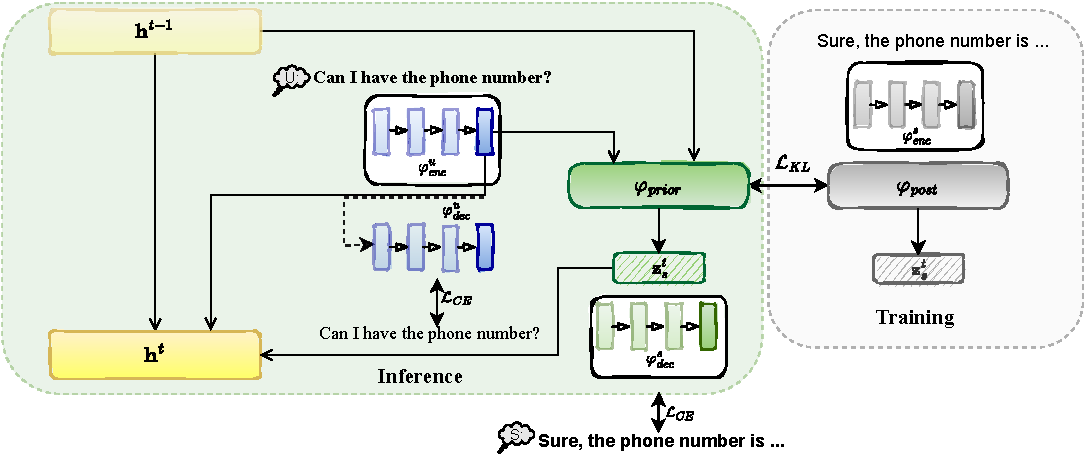
\includegraphics[width=0.9\textwidth]{images/vrnn-diagram.pdf}
    \caption{Visualization of our model architecture (one dialogue turn), described in Section~\ref{05:sec:vrnn-model}. Yellow boxes represent the turn-level VRNN's hidden state $h^t$. The user utterance is represented as the last hidden state of the encoder network $\varphi_{enc}^u$, which is trained as an autoencoder along with the decoder $\varphi_{dec}^u$. The system utterance, encoded by the network $\varphi_{enc}^s$, is an input to the posterior network $\varphi_{post}$ that helps to train the prior network $\varphi_{prior}$ to construct meaningful latent variables $\mathbf{z}_s$, which initialize the system utterance decoder $\varphi_{dec}^s$. The training uses the whole architecture, including the posterior network $\varphi_{post}$, while only the part shaded in green is used for inference. $\mathcal{L}_{CE}$ stands for cross-entropy loss, $\mathcal{L}_{KL}$ for KL-divergence loss.}
    \label{05:fig:vrnn_method}
\end{figure}

\subsection{TO-VRNN model description}
\label{05:sec:vrnn-model}
We extend the VRNN model introduced in Chapter \ref{02:sec:vrnn} to fit the task-oriented setup.
Figure \ref{05:fig:vrnn_method} depicts our model's architecture.
Following the original VRNN architectures (Section~\ref{02:sec:vrnn}), we employ a turn-level RNN that summarizes the context in its hidden state.
In each dialogue turn, we model user and system utterances with separate autoencoders to account for different user and system behaviors.
This contrasts with the original model described in~\ref{02:sec:vrnn}, which contains only one autoencoder in every time step.
We can divide the processing of one turn into two stages.
First, the user utterance, modeled with a standard vanilla autoencoder, is processed, and the last encoder hidden state $\varphi^u_{enc}(\mathbf{x}^t_u)$ provides the encoded representation used as an input for the next stage.

Next, the system part is used, which is realized by VAE with discrete latent variables $\textbf{z}_s$ conditioned on the context RNN's hidden state $\mathbf{h}^{t-1}$ and the user utterance encoding $\varphi^u_{enc}(\mathbf{x}^t_u)$.
The system module is trained as the VAE component in the VRNN model (\ref{02:sec:vrnn}) and creates latent representations interpreted as system actions.
This predicted latent variable is then used as an input to the system decoder that generates the realization of the latent action in the form of natural language.
Our model can thus be seen as a VRNN extended by an additional encoder-decoder module for input pre-processing.

To finalize the turn-processing step, we need to save the information into the turn-level network so it becomes part of the encoded context.
The turn-level network state update looks as follows:
\begin{equation}
    \begin{gathered}
        \mathbf{h}^{t+1} = \text{RNN}([\varphi^u_{enc}(\mathbf{x}_u^t),\varphi_{z}(\mathbf{z}^t_s)], \mathbf{h}^t)
    \end{gathered}
\end{equation}
In other words, we use representations from both user and system modules to pass the information necessary to update the overall state.

For word-level encoding and decoding modules ($\varphi_{enc}^u,\varphi_{enc}^s,\varphi_{dec}^u,\varphi_{dec}^s$), we use an RNN with LSTM cells.
We further experiment with attention \cite{bahdanau2014neural} over user encoder hidden states in the system decoder.
We train the model by minimizing a sum of the cross-entropy reconstruction loss on user utterances and the variational lower bound (Equation~\ref{eq:elbo}) on system responses.
\begin{equation}
\begin{split}
    \log~p(\mathbf{x}) \ge -\mathrm{KL}(q(\mathbf{z}|\mathbf{x})||p(\mathbf{z}))\\ + \mathbb{E}_{q(\mathbf{z}|\mathbf{x})}[\log~p(\mathbf{x}|\mathbf{z})]
    \label{eq:elbo}
\end{split}
\end{equation}
The final objective is presented in Equation~\ref{eq:loss-to-vrnn}.
There, $\phi$ and $\psi$ represent the parameters corresponding to system and user modules, respectively. $\mathbf{x}_s$ and $\mathbf{x}_u$ are system and user utterances and $\mathbf{u}$ is the encoded representation of the user utterance.
\begin{equation}
\begin{split}
    \mathbb{L}_{TO-VRNN}(\phi,\psi) = \mathbb{E}_{q_{\phi}(\mathbf{z}|\mathbf{x}_s)}[\log~p_{\phi}(\mathbf{x}_s|\mathbf{z})] \\
    -\mathrm{KL}(q_{\phi}(\mathbf{z}|\mathbf{x}_s)||p(\mathbf{z}))\\
    + log~p_{\psi}(\mathbf{x}_u|\mathbf{u})
\end{split}
    \label{eq:loss-to-vrnn}
\end{equation}
This objective directly extends the original training objective presented in \ref{02:sec:vrnn}.

When running in inference mode, only the prior distribution $p(\mathbf{z})$ is considered, which does not require the system utterance on the input.
Therefore, the model can generate the system response only with a user utterance on the input.

\paragraph{Latent Variables}
\label{05:sec:method_latent}
We use a set of $n$ \mbox{$K$-way} $(K=20;n=1,3,5)$ categorical variables to achieve good interpretability, following \citet{zhao2018unsupervised}.
This means that each variable is represented as a one-hot vector of length $K$, and we use $n$ such vectors.
Multiple ways exist to incorporate trainable discrete variables into a differentiable network (see Chapter~\ref{02:sec:vae_discrete}).
We use the Gumbel-Softmax distribution and the reparameterization trick \cite{jang2017categorical}.
We always take the item with the maximum probability concerning the predicted softmax distribution instead of sampling from it during inference.

\subsection{TO-VRNN Experiments}
In this section, we evaluate the quality of responses generated by our model.
We also inspect the model performance concerning dialogue success.
We focus on theoretical modeling and feasibility at this stage, which we believe is sufficiently demonstrated by corpus-based evaluation complemented by manual checks. Detailed interpretation of the learned representations follows in Section~\ref{05:sec:latents}.

\subsubsection{Data}
\label{05:sec:data}

We evaluate the model performance on three datasets: CamRest676 \cite{wen2016network}, MultiWOZ 2.1 (MW)\cite{budzianowski2018multiwoz,eric2019multiwoz} and Stanford Multidomain Dialogues (SMD) \cite{eric-etal-2017-key}
We use standard splits for MultiWOZ 2.1 and SMD.
We split CamRest676 in the 8:1:1 ratio, following previous work.
Detailed descriptions are given in Section \ref{02:sec:input-data-desc}.

\paragraph{Database queries} To include database information in the dialogues as described in Section~\ref{05:sec:to-unsup}, we first identify all turns in the original datasets where database information is required, using handcrafted rules.
These rules are very simple, and their creation requires minimal effort: whenever database results are provided in the data (based on simple pattern matches over system actions), we prepend a database query based on the ground truth state. The assumption is that these queries would naturally be available in a real-world scenario -- database queries induced by human operators can be logged along with client-operator conversations.
We then build database query turns based on the respective state annotation (see example in Table~\ref{05:tab:example}).
Note that database query parameters are the only annotation used to train our models apart from utterance texts; no other dialogue state annotation from the original datasets is used.

\subsubsection{Experimental Setup}
\label{05:sec:expe_setup}
We evaluate two versions of our model: one that uses the attention mechanism (\emph{attn}) and one without it (\emph{noattn}). The number and size of the variables are set based on a few cursory checks on the training data. Our models use ten latent variables by default; we discuss the influence of the number of latent variables in Table \ref{05:z_counts}.
Since our approach is the first to be evaluated in a task-oriented setting with minimal supervision, comparing it to prior works is difficult. Setups with full dialogue-state supervision are not comparable, and dialog-state metrics are not applicable without turn-level supervision. Therefore, we compare our models to standard architectures, such as vanilla LSTM or Transformer encoder-decoder, predicting sequentially using the same amount of supervision as our approach. We also compare to the HRED/VHRED models, perhaps the closest prior work to our approach. To put the results into perspective, we also include scores for fully supervised state of the art on our datasets.
However, note that these scores are not directly comparable.

\paragraph{Training details}
The model is trained with gradient descent using the ADAM optimizer.
We set the hyperparameters according to the BLEU and perplexity results of a grid search on the development set.
The utterance encoder and decoder hidden sizes are 250; the context-LSTM hidden size is 100.
The latent variables are 20-dimensional vectors; their number differs across experiments.
For the RNN components, we use a dropout probability of $0.3$.
The total model size is 7,047,529 parameters.
The training time is 3-8 hours using one GPU, depending on the dataset.
The training is sensitive to some parameters, such as the \nobreak{Gumbel-softmax} temperature, but otherwise, the model trains easily using conventional optimization methods.
To address the issue of posterior collapse (see Section~\ref{background:vae-problems}), we experiment with various approaches to KL annealing.
In our experiments, we use a liner annealing schedule, increasing the $\beta$ annealing coefficient from 0 $\rightarrow$ 1.
\paragraph{Metrics}
We use common metrics described in Table~\ref{05:automatic_metrics}).
To evaluate the quality of individual responses, we compute BLEU score and perplexity on the test set.
Without dialogue-state supervision, we cannot measure task-oriented metrics such \emph{joint goal accuracy}.
Therefore, we decided to measure dialogue success and entity match rate, which we adjusted to the minimally supervised case (details follow).
We also measure the database query accuracy.


\subsection{Results}
\subsubsection{Response quality}
Our architecture performs substantially better than (V)HRED, which commonly fails to acquire the necessary knowledge, especially on larger datasets.
The attention-based versions perform better on BLEU but lose slightly on perplexity.
Comparing HRED and VHRED shows that using the variational approach improves overall performance.
While the GPT-2 PLM outperforms our approach on perplexity, it is worse on BLEU score despite its huge capacity.

We compare to other relevant related works:
\begin{enumerate}
\item \citet{shi2019unsupervised} do not use their model for response generation, but they report a negative log-likelihood of approximately $5.5 \cdot 10^{4}$ when reconstructing the CamRest676 test set. Our \emph{TO-VRNN-noattn} model obtained $0.87 \cdot 10^{4}$, which suggests a better fit of the data.\footnote{This comparison is only approximate since the exact data split is not described by \citet{shi2019unsupervised} -- we can only use a test set of the same size, not the exact same instances.}
\item \citet{wen2017latent} measure response generation BLEU score on fully delexicalized CamRest676 data. Their best-reported result is 24.60, while our model gets 27.23 (30.10 with attention).
\end{enumerate}

Our models can generate relevant responses based on manual checks in most cases.
As expected, only the models, including database turns, can predict correct entities (cf.~Section~\ref{sec:emr}).
A relatively common error is informing about wrong slots, e.g., the model provides a phone number instead of an address or, even more frequently, provides wrong slot values (cf.~Table~\ref{05:tab:example-cont}).

\begin{table}[tp]
    \centering\footnotesize
    \begin{tabular}{l|c|rrrr|rrrr}
      \toprule
      model &  & \multicolumn{4}{c|}{\textbf{CamRest676}}  & \multicolumn{4}{c}{\textbf{MultiWOZ~2.1}} \\
      & db & BLEU & Ppl & MI & EMR &  BLEU & Ppl & MI & EMR \\
    LSTM & \textcolor{red}{\xmark} & 3.90 & 5.34 & -- & -- &  0.92 & 8.23 &
    -- & --\\
    Transformer & \textcolor{red}{\xmark} & 4.98 & 7.72 & -- & -- & 0.95 & 6.95 & -- & -- \\
    GPT-2 & \textcolor{red}{\xmark} & 15.40  & 1.18 & -- & -- & 9.40 & 2.77 & -- & -- \\
    GPT-2 & \textcolor{green}{\cmark} & 13.89 & 1.80 & -- & -- & 9.56 & 2.43 & -- & -- \\
    HRED & \textcolor{red}{\xmark} & \pz2.70 & 13.92 & -- & 0.02 & \pz2.98 & 29.61 &
    -- & 0.01\\
    VHRED & \textcolor{red}{\xmark} & \pz4.34 & 11.76 & 0.21 & 0.02 & \pz4.65 & 32.74 & 0.15 & 0.01 \\
    VHRED & \textcolor{green}{\cmark} & \pz8.50 & 10.23 & 0.17 & 0.36 & 3.82 & 16.61 & 0.07 & 0.04 \\
    \hdashline[0.5pt/2pt]
    TO-VRNN-noattn & \textcolor{red}{\xmark} & 12.98 & \pz4.64 & 0.29 & 0.01 & \pz7.18 & \pz9.16 & \bf0.42 & 0.02\\
    TO-VRNN-noattn & \textcolor{green}{\cmark} & 15.10 & \pz4.45 & \bf0.34 & 0.24 &  11.3 & \pz5.17 & 0.27 & 0.05\\
    TO-VRNN-attn & \textcolor{red}{\xmark} & \bf17.37 &\pz 5.07 & 0.16 &  0.09 & \bf12.28 & 10.19 & 0.06 & 0.04\\
    TO-VRNN-attn & \textcolor{green}{\cmark} & 17.10 & \pz\bf4.23 & 0.22 & \bf0.81 & 11.86 & \bf\pz6.03 & 0.05 & \bf0.08\\
    \hdashline[0.5pt/2pt]
    \emph{supervised $^{*}$} & \textcolor{green}{\cmark} & 25.50  & -- & -- & -- & 19.40 & 2.50 & -- & -- \\
    \bottomrule
  \end{tabular}
    \begin{tabular}{l|c|rrr}
      \toprule
      model &  & \multicolumn{3}{c}{SMD} \\
      & db & BLEU & Ppl & MI  \\
    LSTM & \textcolor{red}{\xmark} & 1.62 & 7.84 & -- \\
    Transformer & \textcolor{red}{\xmark}  & 1.53 & 6.33 & -- \\
    GPT-2 & \textcolor{red}{\xmark} & 9.26 & 2.46 & -- \\
    GPT-2 & \textcolor{green}{\cmark} & 4.54 & 2.02 & -- \\
    HRED & \textcolor{red}{\xmark} & \pz1.25 & 12.50 & -- \\
    VHRED & \textcolor{red}{\xmark} & \pz3.75 & 11.94 & 0.20 \\
    VHRED & \textcolor{green}{\cmark} & 3.94 & 11.86 & 0.19 \\
    \hdashline[0.5pt/2pt]
    TO-VRNN-noattn & \textcolor{red}{\xmark} & \pz7.35 & \pz6.18 & \bf0.53 \\
    TO-VRNN-noattn & \textcolor{green}{\cmark} & \pz9.24 & \pz\bf6.01 & 0.47 \\
    TO-VRNN-attn & \textcolor{red}{\xmark} & 12.30 & \pz6.36 & 0.04 \\
    TO-VRNN-attn & \textcolor{green}{\cmark} & \bf12.40 & 6.11 & 0.11 \\
    \hdashline[0.5pt/2pt]
    \emph{supervised$^{*}$} & \textcolor{green}{\cmark}& 14.40 & -- & --  \\
    \bottomrule
  \end{tabular}
  \caption{Model performance in terms of BLEU for generated responses, Perplexity (Ppl), and Mutual Information (MI) between the generated response and the latent variables $\mathbf{z}_s$. 
  We do not evaluate the database-enriched models on SMD as SMD's database structure does not map easily to our annotation style. 
  We measure MI only for the models that use latent variables explicitly. The \emph{db} column indicates systems that use database information. $^{*}$Note that the supervised state-of-the-art scores are not directly comparable, as the systems use full turn-level supervision.\cite{qin2020dynamic}; }
  \label{05:automatic_metrics}
\end{table}
\begin{table*}[tp]
    \centering\scriptsize
    \begin{tabular}{crp{0.6\linewidth}}
        \toprule
         \multirow{4}{*}{\bf Turn 1}&\bf user:& \texttt{Is there a \textbf{moderately priced} restaurant serving \textbf{italian} food anywhere in town?} \\
         &\bf system gold: & \texttt{query italian moderate} \\
         &\bf system hyp: & \texttt{query \textbf{\textcolor{darkgreen}{italian moderate}}}  \\
         \midrule
        \multirow{4}{*}{\bf Turn 2}&\bf user/database:& \texttt{pizza express, Regent Street City Centre, 01223 324033, C.B 2, 1 D.B, centre}  \\
         &\bf system gold:& \texttt{Pizza express serves Italian food and is located in the town centre and is in the moderate price range .} \\        
        &\bf system hyp:& \texttt{\textbf{\textcolor{red}{Pizza hut Cherry Hinton}} is a Italian restaurant in the \textbf{\textcolor{darkgreen}{centre}} part of town} \\
         \midrule
        \multirow{4}{*}{\bf Turn 3}&\bf user:& \texttt{what is the \textbf{address} and \textbf{phone number} ?} \\
        &\bf system gold:& \texttt{their address is  Regent Street City Centre. Their phone number is 01223 324033. can I help with anything else ?} \\
        & \bf system hyp:& \texttt{the phone number is \textbf{\textcolor{darkgreen}{01223 324033}}. Is there anything else I can help you with ?} \\
        \bottomrule
    \end{tabular}
    \vspace{-2mm}
    \caption{Predicted outputs or our VRNN model for a conversation snippet presented in~\ref{05:tab:example}}
    \label{05:tab:example-cont}
\end{table*}

\paragraph{Dialogue success}
The dialogue success or \emph{success rate} reflects the ratio of dialogues in which the system captures all the mentioned slots correctly and provides all the requested information.
We follow previous works \cite{nekvinda2021shades} and report corpus-based success scores instead of using a user simulator.
However, measuring success rate without turn-level labels is not straightforward.
We approximate tracking slot values turn-by-turn by checking for correct slot values upon database queries only, and we use this information to measure dialogue success.
Note that this is not equivalent to having state tracking labels available at all turns, but we consider it a reasonable approximation given our limited supervision -- database queries are crucial for presenting the correct entities to the user, which in turn decides the dialogue success.

The generated query attributes directly show the captured slots.


Success rate results are shown in Table~\ref{tab:success}.
Our system is not competitive with a fully supervised model but outperforms the baselines (VHRED, GPT).
Upon inspection,
we see that the system is often able to recognize correct slots.
However, it has difficulties capturing the correct values.
However, the scores are promising, considering the minimal supervision of our training.

\begin{table}[tp]
    \centering\small
    \begin{tabular}{lcc}
      \toprule
      model &  success & query acc.\hspace{-2mm} \\
      \midrule
      \multicolumn{3}{c}{\textbf{CamRest676}} \\
      \midrule
      VHRED & 0.21 & 0.91 \\
      TO-VRNN-noattn & 0.28 & 0.84 \\\hdashline[0.5pt/2pt]
      supervised SotA \cite{peng2021soloist}\hspace{-2mm} & 0.73 & N/A \\
      \midrule
      \multicolumn{3}{c}{\textbf{MultiWOZ}} \\
      \midrule
      TO-VRNN-noattn & 0.10 & 0.98 \\\hdashline[0.5pt/2pt]
      supervised SotA \cite{peng2021soloist}\hspace{-2mm} & 0.85 & N/A \\
      \bottomrule
  \end{tabular}
  \caption{Dialogue success and query accuracy comparison for VHRED, \emph{TO-VRNN-noattn} using the database and a state-of-the-art supervised system.}
  \label{tab:success}
\end{table}

\paragraph{Matching database entities}
\label{sec:emr}
Table~\ref{05:automatic_metrics} shows the performance of our models for entity matching.
We observe that the model performance without the database information is poor.
However, including the database information improves the performance substantially, especially in the case of CamRest676 data.
The MultiWOZ data is much more complex -- it contains more slots and multiple domains that can also be combined in an individual dialogue.
Nevertheless, we can still observe an improvement when we include the database queries.
We also note that using attention improves EMR substantially -- the latent variables alone cannot hold all information about particular values (cf.~Section~\ref{sec:pred_latents}).

\paragraph{Database query accuracy}
Further, we evaluate the accuracy of the database querying.
This metric measures if the system queries the database at appropriate turns.
The query's content is not considered in this case, as it is already considered in the success rate.
On MultiWOZ, we get a near-perfect accuracy, while our approach loses to VHRED on CamRest676 (see Table~\ref{tab:success}).
We hypothesize that different dialogue structures can cause such discrepancies among these two datasets.
The dialogues in CamRest676 usually contain just zero or one query during a dialogue, so our model might generate more queries than necessary.

\subsection{Latent Variable Interpretation}

\label{05:sec:latents}
\begin{table}[tp]
    \centering\small
    \begin{tabular}{l|ccc}
      \toprule
      & BLEU & Ppl & MI  \\
    \midrule
    TO-VRNN-noattn-1z  & 25.20 & 4.25 & 0.46  \\
    TO-VRNN-noattn-3z  & 26.80 & 4.24 & 0.26  \\
    TO-VRNN-noattn-5z  & 27.23 & 4.20 & 0.38  \\
    TO-VRNN-noattn-12z  & 29.83 & 4.12 & 0.35  \\    

    \bottomrule
  \end{tabular}
  %\vspace{-2mm}
  \caption{Evaluation of the model performance with different numbers of latent variables concerning automatic measures of BLEU, Perplexity (Ppl), and Mutual Information (MI) on the CamRest676 data.}
  \label{05:z_counts}
\end{table}
We believe that explaining and interpreting the model behavior is crucial, especially in a setting without full supervision.
Therefore, we design experiments to evaluate the model behavior and investigate whether the model captures salient dialogue features in the latent variables obtained during training on CamRest676 and MultiWOZ.
While the latent variables seem to be mainly useful for interpretability or structure induction, they are likely also contributing to the performance as smaller latent spaces yield lower performance, as shown in Table~\ref{05:z_counts}.

\subsubsection{Mutual Information}
Finally, we compute mutual information (MI) between the generated text and latent variables as well as among the latent variables themselves (see Table~\ref{05:automatic_metrics}).\footnote{
Since we measure MI between categorical variables, we quantize the continuous variables used in the VHRED model.}
We see that using attention dramatically affects the amount of MI between the latent variables and the generated text.
It appears that since attention bypasses the latent vectors, the decoder does not need to use them to store information.

\subsubsection{Clustering the actions}
\label{sec:clustering}
First, we want to assess whether similar variables represent similar actions.
We follow \citet{zhao2018unsupervised} and define utterance clusters according to the model's latent variables.
As a baseline, we consider random cluster assignment.
A stronger approach computes sentence representations using a BERT model tuned for sentence representations \cite{reimers-2019-sentence-bert} and then clusters the obtained sentence embeddings using K-means clustering.

We then use the homogeneity metric \cite{rosenberg-hirschberg-2007-v} to evaluate the clustering quality for the reference classes determined by manually annotated system actions (which are used for evaluation only).
Homogeneity reflects the information the clustering provides (and, by extension, the latent vectors used) and is normalized to the interval [0, 1].
The reason for choosing this metric is that it is independent of the number of labels and their permutations.
If all clusters only contain instances of a single class, we get the maximum homogeneity.

We provide the results in Table~\ref{tab:homo}.
The clusters formed on the CamRest676 data are more homogeneous than MultiWOZ, likely because of the greater dataset complexity in the latter case. 
In all cases, our clusters are much more homogeneous than clustering formed by random assignment.
We also compare favorably to a stronger baseline based on the clustering of the sentence representations.
These results suggest that the representations formed by our model correspond much better to the true actions seen in the data.

\begin{figure*}[t]
    \centering
    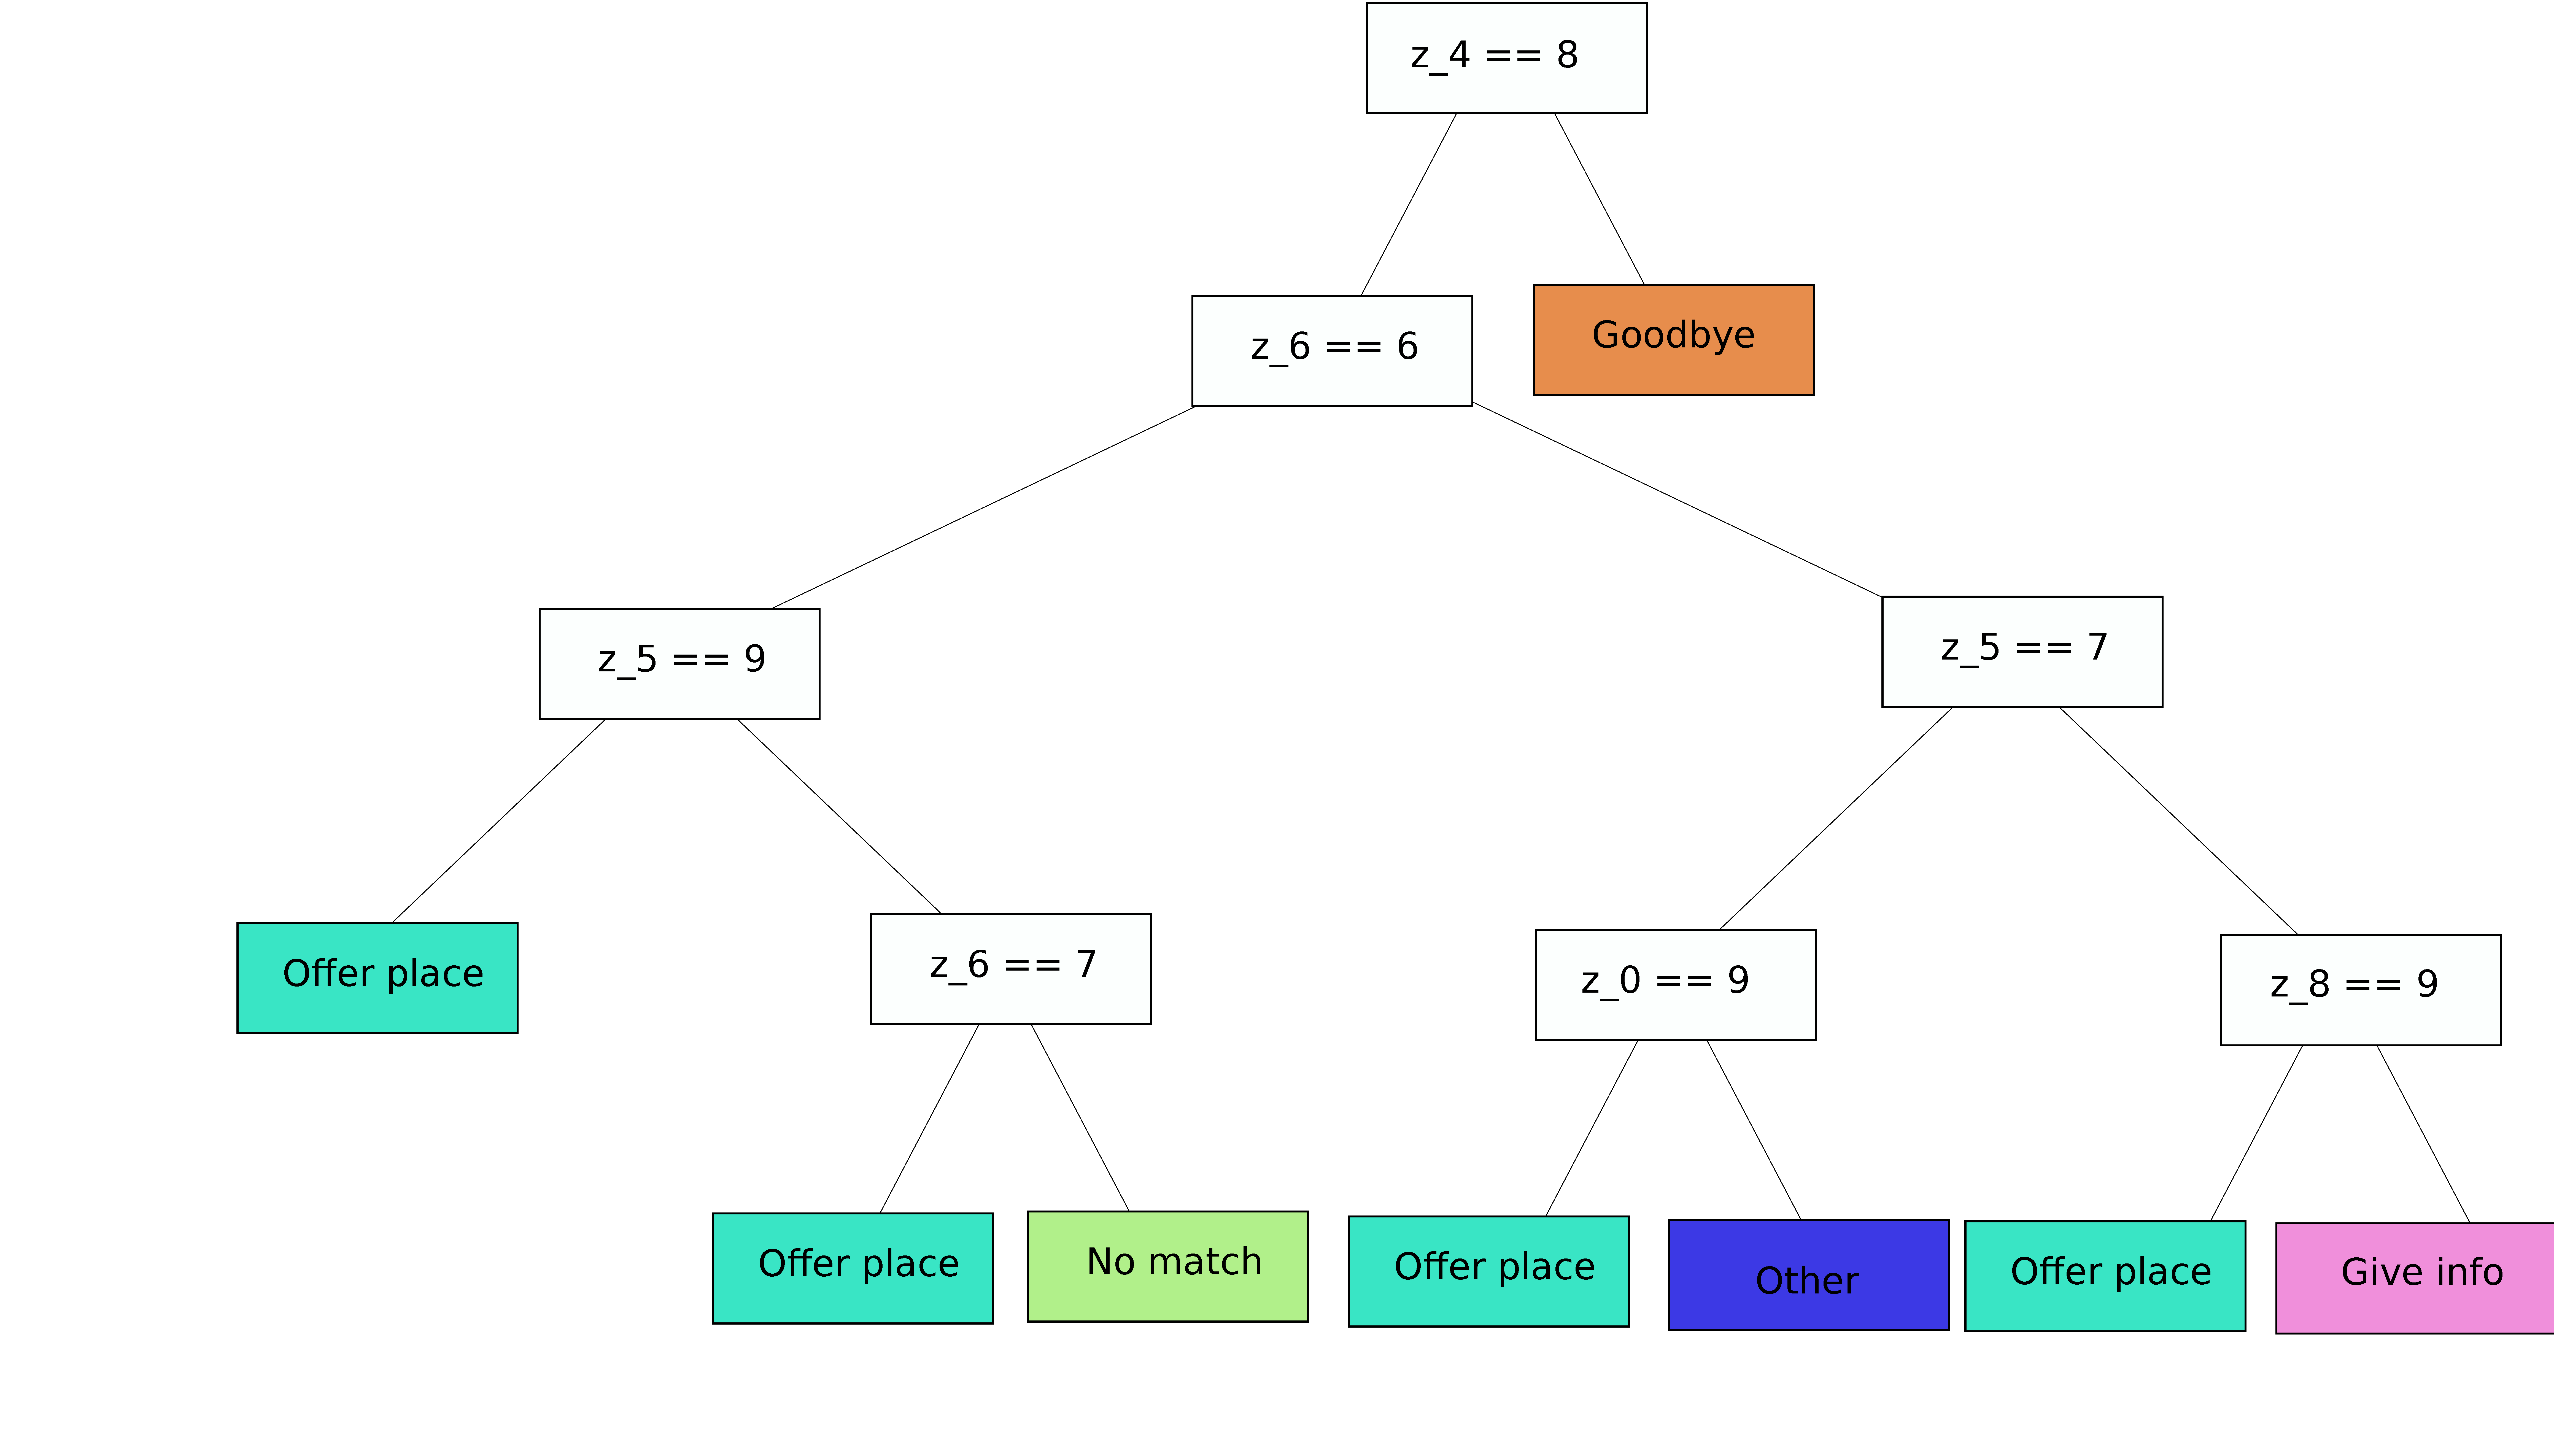
\includegraphics[width=0.70\textwidth]{images/dt2.pdf}
    \vspace{-5mm}
    \caption{A visualization of a decision tree trained on the CamRest676 data to predict a system action from the contents of the latent variables. Each node represents a decision based on one latent variable value, and the leaf node colors represent different system actions. When the condition in a given node is fulfilled, the algorithm proceeds into the right subtree, left otherwise. For clarity, we limit the maximum tree depth to 4. The limit slightly lowers the accuracy -- the pictured tree achieves an accuracy of 73\% on the CamRest676 data.}
    \label{fig:dt}
\end{figure*}

\subsubsection{Predictive power of the variables}
\label{sec:pred_latents}
\begin{table}[tp]
    \centering\small
    \begin{tabular}{l|c|cc}
      \toprule
      config & \textbf{CamRest676} & \multicolumn{2}{c}{\textbf{MultiWOZ 2.1.}} \\
       & gold & domain & action \\
      \midrule
      random  & 0.17 & 0.14 & 0.09 \\
      majority &  0.42 & 0.33 & 0.32 \\\hdashline[0.5pt/2pt]
      HRED & 0.65 & 0.45 & 0.44 \\
      VHRED & 0.52 & 0.36 & 0.32 \\
      GPT-2 & 0.65 & 0.60 & 0.55 \\
      %TO-VRNN-3z & 0.648 & 0.599 & 0.543 \\
      TO-VRNN-attn & 0.63 & 0.68 & 0.66 \\
%     TO-VRNN-5z (LR) & 0.721 &  & \\
      TO-VRNN-noattn & \textbf{0.75} &  \textbf{0.70} & \textbf{0.69} \\\hdashline[0.5pt/2pt]
      TO-VRNN-manual & 0.59 & -- & -- \\
      %10z (DT) & \textbf{0.759} & \textbf{0.641} & \textbf{0.404} \\
      %10z-attn (DT) & 0.597 & 0.460 & 0.296 \\

      \bottomrule
  \end{tabular}
  \caption{Accuracy of the domain and action decision-tree classifiers based on latent variables. 
  For details about the manual annotation process, see Section~\ref{sec:manual}.}
  \label{tab:latent_classification}
\end{table}
To evaluate the predictive power of the obtained latent representations, we train a simple classifier that predicts the system action and current domain, using solely the obtained latent representations as input features.
CamRest676 data does not include system action annotation.
Hence, we manually designed a set of rules to determine system actions.
An example of this rule-based action annotation is shown in Table~\ref{05:tab:example}.
For MultiWOZ, we predict both system action and the domain of the utterance.

To put our results into perspective, we include several baselines: trivial random and majority class baselines and classifiers using representations obtained with other methods (HRED, VHRED, GPT).
We use a decision tree (DT) classifier trained with the CART algorithm\footnote{\url{https://scikit-learn.org/stable/modules/tree.html}} and the \emph{gini} split criterion due to its good interpretability.
The results are shown in Table~\ref{tab:latent_classification}.
Our classifier beats the random and majority baselines in all cases.
It also outperforms classification based on (V)HRED and GPT representations.
This demonstrates that our approach produces high-quality interpretable representations.
We also observe that using attention harms the performance of the action classifier as it makes it possible for the models to bypass the latent variables.
On CamRest676, the latent variables explain most of the annotated actions.
Overall, we can observe that any hidden state taken from some trained model can explain some portion of the data.
However, using our approach seems to perform better in this aspect.
We also notice the influence of the number of latent variables on the performance.
In general, increasing the number of latent variables leads to a substantial performance improvement, which suggests that all the variables contribute with relevant information (see Table~\ref{tab:latent_classification}).

The information about domains and system actions is stored in categorical variables and can be extracted by a simple classification model such as the decision tree, which allows us to interpret and explain the behavior of our model.
For illustration, in Figure \ref{fig:dt}, we plot a DT with limited depth that achieves 73\% accuracy when predicting the system action on the CamRest676 data.
The aim is that latent variables hold high-level information, such as intents, actions, or domains. This helps interpretability but is insufficient for generating appropriate and factually correct responses -- here, we need to incorporate correct slot values.
This detailed information is captured and carried over via the attention mechanism in \emph{TO-VRNN-attn}.
Potential alternatives are copy mechanisms \cite{lei2018} or delexicalization on the generated outputs \cite{henderson_robust_2014,peng2021soloist}.

\subsubsection{Manual interpretation}
\label{sec:manual}
To explore the interpretability of our representations even further, we manually annotate the latent variables to obtain a simple handcrafted classifier.
Specifically, we draw a set of pairs of utterances and corresponding latent representations from the validation set.
We present the discrete representation vectors to an expert annotator to assign an action that each vector represents based on the sampled utterances.
This way, we obtain a mapping from the space of latent vectors to actions.
We then apply this mapping to predict actions on the test set (the \textit{TO-VRNN-manual} entry in Table \ref{tab:latent_classification}).
Note that in this approach, we only allow assigning an action to a whole vector, unlike in the case of a decision tree classifier which can take individual components into account.
As the results show, this approach works well despite the above limitation.

\begin{table}[tp]
    \centering\small
    
\begin{tabular}{l|c|c|c}
      \toprule
      \textbf{Source} &\textbf{ CamRest action} & \textbf{MW action} & \textbf{MW domain} \\
      \midrule
      TO-VRNN-noattn & 0.65 & 0.34 & 0.39 \\
      sent-repr & 0.45 & 0.33 & 0.30 \\
      random & 0.20 & 0.02 & 0.01 \\
      \bottomrule
  \end{tabular}
  \caption{Homogeneity for \emph{TO-VRNN-noattn} configuration using the database vs.~a clustering of sentence representations and random baseline.}
  \label{tab:homo}
\end{table}

\section{Hierarchical Variational Model for TOD (HVTOD)}
A structured representation of utterances in the dialogue with dialogue acts (Chapter~\ref{02:sec:basics}) is hierarchical because it is a composition of several concepts that can constrain each other.
Specifically, each utterance is characterized on the top level by its domain.
Each domain is connected with some intents and system actions, typically further connected with certain slots.
To reflect this hierarchical nature of the dialogue acts, we thus need some model that would structure its representations accordingly.
Since we are interested in latent representations, VAE architecture is a good option thanks to reasons discussed in \ref{05:fig:vrnn_method}.

VAEs for hierarchical architecture were successfully applied in the computer vision domain \cite{vahdat2020nvae,li2020progressive}.
We take inspiration from these works and apply the hierarchical variational autoencoder architecture to the dialogue domain.
We hypothesize that this structure will allow the model to work with different levels of abstraction and thus represent the decision process more accurately and with greater detail.
Note that there is no guarantee that the learned representations in different layers will also differ.
We want to explore this question to see if the model can learn to leverage this structure by itself. 

\subsection{HVTOD model architecture}
\begin{figure}[h]
    \centering
    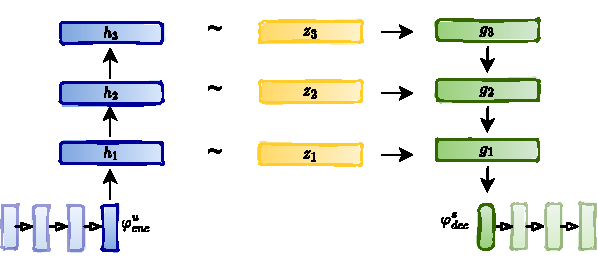
\includegraphics[width=0.9\textwidth]{images/HVTOD-full-noN.pdf}
    \caption{The architecture of our HVTOD model. The dialogue context is first processed with a recurrent network encoder to obtain a hidden representation. This representation then serves as an input to the hierarchical system of variational encoders stacked on each other. The latent variables are merged to form the decoder's initial hidden state.}
    \label{05:fig:HVTOD-full}
\end{figure}
The proposed HVTOD architecture is based on the LAVA framework (\cite{lubis-etal-2022-dialogue}, see Section~\ref{02:sec:lava}).
In LAVA, the authors propose an architecture that uses latent representations of dialogue actions computed with VAE.
They use context encoded with an RNN encoder as an input into the VAE.
We extend the architecture so that instead of just one VAE.
We use a set of VAEs stacked on top of each other to model the latent variables.
The overall model architecture is depicted in Figure~\ref{05:fig:vrnn_method}.
In the input, we have a set of dialogues $\mathcal{D}$ where each dialogue $d$ with $n$ turns consists is represented as a sequence of altering system and user utterances $d = (s_1,u_1,...,s_n,u_n)$.
Similarly to LAVA, our model encodes the context $C^t = (s_1,u_1,...,s_t,u_t)$ with RNN-based utterance encoder to obtain a hidden representation of the context $h_0 = RNN_{\varphi_{enc}^u} (C^t)$.
The obtained representation $h_0$ is subsequently used as input to a hierarchical $L$ variational autoencoder system.
The autoencoders are stacked on each other.
Therefore, we refer to $l-th$ VAE as VAE on level $l$ or sometimes just \emph{layer l}.
Formally, each level $l$ computes parameters of posterior distribution $q(z_l|C^t)$ to sample the latent variable as follows:
\begin{equation}
\begin{split}    
    \mathbf{h}_l = e_l(\mathbf{h}_{l-1}) \\
    \mathbf{z}_l~\mathtt{\sim}~p(\mathbf{z}_l|C^t) = q_l(\mathbf{h}_l) \\
\end{split}
\end{equation}
where $e_l, A_l$ are trainable matrices.
In other words, each latent variable $z_l$ on level $l$ is sampled from a  distribution conditioned on context and preceding VAE layers $q(z_l|C^t,h_1,...,h_{l-1})$.
We use Gumbel-softmax distribution to obtain discrete vectors similar to the previous section.
To form the output, we aggregate the information on each layer in an output variable $g_l$ as follows:
\begin{equation}
\mathbf{g}_l = D_l(z_l) + \alpha \cdot \mathbf{g}_{l+1}, \alpha_l \in [0, 1]
\end{equation}
Where $\alpha_l$ is a scaling coefficient increased during training. All $\alpha_l$ are set to 1 in the trained network.
The output from the bottom hidden layer $g_1$ generates the response $s_{t+1}$  using an RNN decoder parametrized by $\varphi^s_{dec}$.

\subsection{HVTOD training}
In the LAVA framework, there are multiple stages of training.
Here, we want to focus on unsupervised pre-training with an auto-encoding objective.
However, we also evaluate the model performance in a supervised setting to understand the behavior better.
\begin{figure}[h]
    \centering
    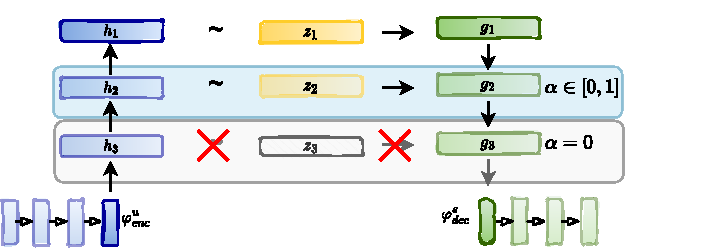
\includegraphics[width=0.9\textwidth]{images/HLAVA-fadein.pdf}
    \caption{Our hierarchical variational model during training. At this stage, the top layer is used completely; the second layer is faded-in with increasing coefficient $\alpha$ while the bottom layer is not used yet, so it is effectively disconnected from the computation graph.}
    \label{05:fig:HVTOD-fadein}
\end{figure}

\subsubsection{Training stages}
We start the training with autoencoding.
For the auto-encoding pre-training, we take an utterance $x$ as input and follow the traditional approach to VAE training.
We minimize the Evidence Lower Bound objective (ELBo), which we extend to reflect multiple levels of VAEs.
The full minimalization objective, therefore, is:
\begin{equation}
    \mathbb{L} = \mathbb{E}_{q(z_1|X^1),...,q(z_L|X^L)}[log~p(x|z_1,...z_L)] - \mathlarger{\mathlarger{\sum}}_{l=0}^L~D_{KL}[q(z_l|X^l)||p(z)]
\end{equation}
Where $X^L = x,z_1,...,z_{L-1}$.

The second stage is fine-tuning the pre-trained model.
We assume that the pre-training task helps to learn the network to create useful representations that can contribute to additional stages of training.
To confirm this, we employ the second stage of training in which we use supervision in the form of belief state labels, which we include in the input.
While in the autoencoding (AE) stage, the model learns to reconstruct the input utterance.
During fine-tuning (FT), the model takes dialogue context and predicts a system response.
FT stage utilizes the decoder pre-trained in the AE stage, and the encoder part is trained from scratch.

\subsubsection{Training specifics}
Training the network comprising multiple VAEs is challenging due to VAE training issues (Section~\ref{02:sec:vae}).
To simplify the training process, we incorporate the layers one by one.
Only the bottom layer is initially trained; more layers are added later.
To achieve this, we introduce a \emph{fade-in coefficient} $\alpha$~\citep{li2020progressive} that is being annealed from $0 \rightarrow 1$ over a predetermined number of steps and serves to incorporate a new layer during training smoothly.
This process is depicted in Figure~\ref{05:fig:HVTOD-fadein}.

Furthermore, we experiment with an additional training objective -- placeholder predictions.
Since we work with delexicalized data, we can train the network to predict which placeholders are present in the utterance.
We include this additional pseudo-supervision in the form of so-called \emph{placeholder loss} $\mathbb{L}_{pl}$, which is computed simply as binary cross-entropy for each placeholder prediction.

\subsection{Experiments}
We are interested in evaluating two aspects of the proposed model.
First, we explore how the multi-layer architecture contributes to the overall performance.
Next, we evaluate the properties of learned latent variables.
We use MultiWOZ 2.1 (See~\ref{02:sec:data-desc}) for training and evaluation.
We delexicalize (see Section~\ref{02:delex}) the utterances for training.

\subsubsection{Unsupervised HVTOD}
The second stage of HVTOD training, the fine-tuning, needs labels as supervision.
We are interested in the task of dialogue response generation when no labels are available.
Therefore, we also train an unsupervised variant of the model.
We base this stage on the auto-encoding objective and employ the same mechanism as auto-encoding but train the model to predict the next response instead of reconstructing it.

\subsubsection{Technical Details}
For training the model, we use a single GPU, NVIDIA A30.
We train the model for 100 epochs using the ADAM optimizer while we observe a decline in the validation loss.
The learning rate is set to $10^{-3}$.
We use discrete latent variables of dimension 20 to represent latent dialogue actions.
We determined the parameters by empirical experiments using grid search.
To get a fair comparison, we adjust the number of latent variables used according to the number of layers in the model hierarchy.
We adjust the number so that each configuration effectively has the same dimension of the latent space.
In the supervised training stage, we represent the belief state as a one-hot discrete vector corresponding to specific slots.

\subsubsection{HVTOD performance}
We evaluate the performance of HVTOD with a different number of layers and with or without the placeholder loss for dialogue response generation in unsupervised (Table~\ref{05:tab:hvtod-unsup}) and supervised (Table~\ref{05:tab:hvtod-ft}) setting.
All variants are first trained with an autoencoding objective.
We also evaluate the model quality after pre-training in Table~\ref{05:tab:hvtod-ae}.

Note that when we increase the number of layers, we decrease the dimension of the latent space accordingly.
Therefore, all the compared models have the same number of parameters.

\paragraph{Autoencoding}
We can see that in the autoencoding setting (Table~\ref{05:tab:hvtod-ae}), the increased number of layers helps to improve the performance concerning dialogue success and BLEU.
Moreover, the dialogue success is also improved by including our additional placeholder loss.

\paragraph{Supervised fine-tuning}
The results of supervised fine-tuning are given in Table~\ref{05:tab:hvtod-ft}.
This way, we achieve much higher scores, as expected.
Also, we can see that the placeholder loss contributes to the overall model performance as does the number of used layers.

\begin{table}[tp]
    \centering
    \begin{tabular}{c|c|c|c}
    \toprule
    \textbf{no layers}& \textbf{placeholder loss} & \textbf{Success-unsup} & \textbf{BLEU-unsup} \\
    \midrule
         1 & \textcolor{red}{\xmark} & 0.20 $\pm$ 0.06 & 15.36 $\pm$ 0.90 \\
         1 & \textcolor{green}{\cmark} & 0.34 $\pm$ 0.06 & 16.43 $\pm$ 0.62 \\
         2 & \textcolor{red}{\xmark} & 0.32 $\pm$ 0.07 & 16.39 $\pm$ 0.67  \\
         2 & \textcolor{green}{\cmark} & 0.33 $\pm$ 0.07 & 16.31 $\pm$ 0.45 \\
         3 & \textcolor{red}{\xmark} & 0.35 $\pm$ 0.03 &  16.67 $\pm$ 0.48 \\
         3 & \textcolor{green}{\cmark} & 0.35 $\pm$ 0.02 & 16.92 $\pm$ 0.84 \\
    \bottomrule
    \end{tabular}
    \caption{The results of HVTOD architecture after fine-tuning on dialogue response generation in an unsupervised setting, i.e. without belief state labels as inputs. We provide means and standard error intervals computed over five runs.}
    \label{05:tab:hvtod-unsup}
\end{table}

\paragraph{Unsupervised response generation}
For the unsupervised response generation (Table~\ref{05:tab:hvtod-unsup}), we observe the benefits of using the placeholder loss when only one-level hierarchy is used.
Surprisingly, we don't observe a similar effect when more layers are employed.
Nevertheless, there are performance gains when using placeholder loss in the supervised setting (Table~\ref{05:tab:hvtod-ft}).
This behavior shows that unsupervised dialogue response generation doesn't benefit from placeholder loss when more layers are employed.
This suggests that one of the layers in a multi-layer hierarchy can capture information that can be gained from placeholder loss.

\subsubsection{Latent space inspection}
We inspect the structure of the learned latent space by transforming the variables using the t-SNE algorithm~\cite{van2008visualizing} into 2-dimensional latent space and plotting them colored by their assignment to respective domains~\cite{lubis-etal-2022-dialogue}.
For autoencoding (Figure~\ref{05:fig:ae-layers}), the placeholder loss shapes the latent space to form more spread homogenous clusters, specifically on layer 1.
The same influence is even more visible when we visualize latent spaces after training the model for dialogue response generation (Figure~\ref{05:fig:ft-layers}).
Although the influence on latent space shape is clear, there is no significant difference in the final performance of the respective models.
We also observe that although each layer contains useful information, there is some overlap between the layers.
This suggests that it might be useful to enforce disentanglement of the latent variables somehow.

\begin{table}[tp]
    \centering
    \begin{tabular}{c|c|c|c}
    \toprule
    \textbf{no layers}& \textbf{placeholder loss} &  \textbf{Success-ft} & \textbf{BLEU-ft} \\
    \midrule
         1 & \textcolor{red}{\xmark} & 0.44 $\pm$ 0.08 & 17.37 $\pm$ 0.53 \\
         1 & \textcolor{green}{\cmark} & 0.52 $\pm$ 0.07 & 18.62 $\pm$ 0.52 \\
         2 & \textcolor{red}{\xmark} & 0.51 $\pm$ 0.03 & 19.17 $\pm$ 0.26 \\
         2 & \textcolor{green}{\cmark} & 0.55 $\pm$ 0.04 & 19.74 $\pm$ 0.36 \\
         3 & \textcolor{red}{\xmark} & 0.52 $\pm$ 0.04 & 19.36 $\pm$ 0.72 \\
         3 & \textcolor{green}{\cmark} & 0.55 $\pm$ 0.04 & 19.63 $\pm$ 0.41 \\
    \bottomrule
    \end{tabular}
    \caption{The results of HVTOD architecture after fine-tuning on dialogue response generation using belief state labels as inputs. We provide means and standard error intervals computed over five runs}
    \label{05:tab:hvtod-ft}
\end{table}

\begin{table}[tp]
    \centering
    \begin{tabular}{c|c|c|c}
    \toprule
    \textbf{No. of layers}& \textbf{placeholder loss}& \textbf{Success} & \textbf{BLEU} \\
    \midrule
         1 & \textcolor{red}{\xmark} & 0.46 $\pm$ 0.02 & 55.39 $\pm$ 1.43 \\
         1 & \textcolor{green}{\cmark} & 0.58 $\pm$ 0.03 & 55.86 $\pm$ 1.17 \\
         2 & \textcolor{red}{\xmark} & 0.50 $\pm$ 0.02 & 59.07 $\pm$ 1.31 \\
         2 & \textcolor{green}{\cmark} & 0.62 $\pm$ 0.01 & 62.42 $\pm$ 1.16 \\
         3 & \textcolor{red}{\xmark} & 0.53 $\pm$ 0.02 & 58.84 $\pm$ 1.46 \\
         3 & \textcolor{green}{\cmark} & \textbf{0.62} $\pm$ 0.01 & \textbf{64.50} $\pm$ 0.96 \\
    \bottomrule
    \end{tabular}
    \caption{The results of HVTOD architecture after pre-training with the unsupervised autoencoding objective. We provide means and standard error intervals computed over five runs. Note that dialogue success, in this case, indicates the reconstruction quality, but the model cannot be used for response dialogue generation since it's only trained on autoencoding.}
    \label{05:tab:hvtod-ae}
\end{table}


\begin{figure}[h]
\centering
\subfloat[level 1]{\label{sfig:a0}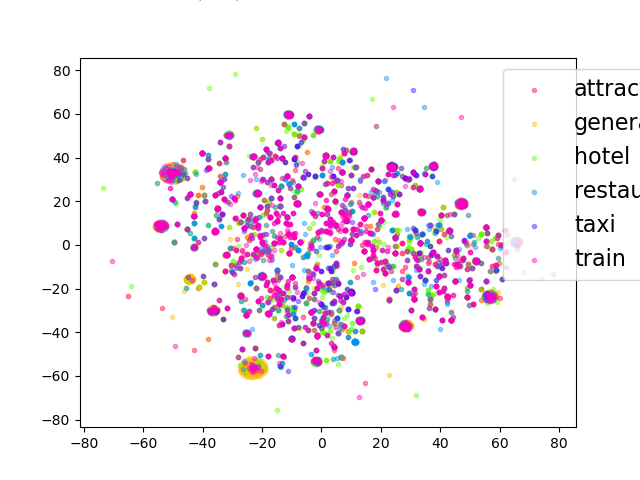
\includegraphics[width=.5\textwidth]{images/lava-tsne/ae-lvl-0-nll.png}}\hfill
\subfloat[level 1 + ph loss]{\label{sfig:b0}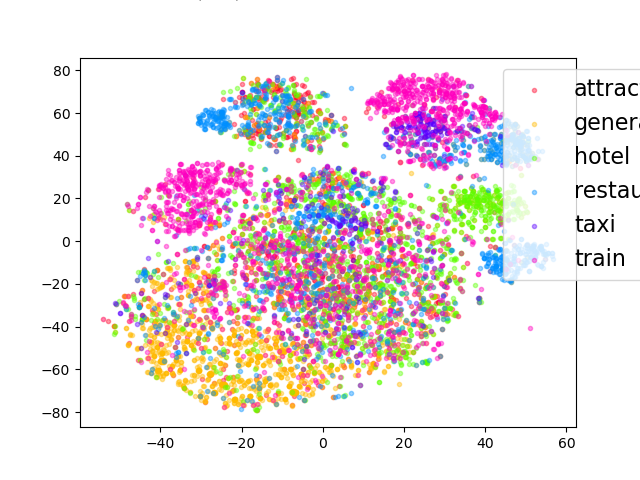
\includegraphics[width=.5\textwidth]{images/lava-tsne/ae-lvl-0-bce.png}}\\

\subfloat[level 2]{\label{sfig:a1}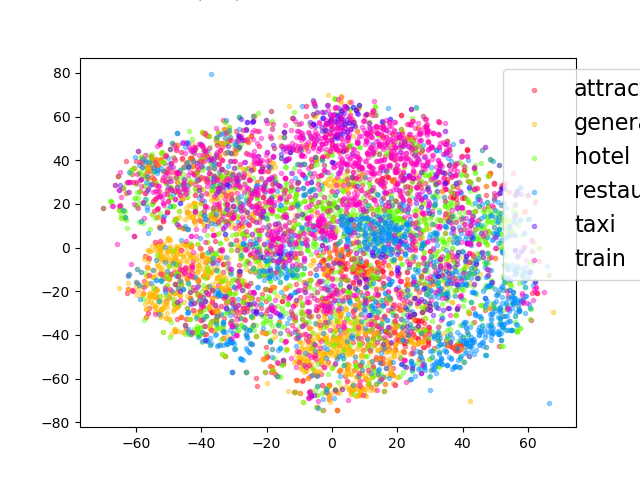
\includegraphics[width=.5\textwidth]{images/lava-tsne/ae-lvl-1-nll.png}}\hfill
\subfloat[level 2 + ph loss]{\label{sfig:b1}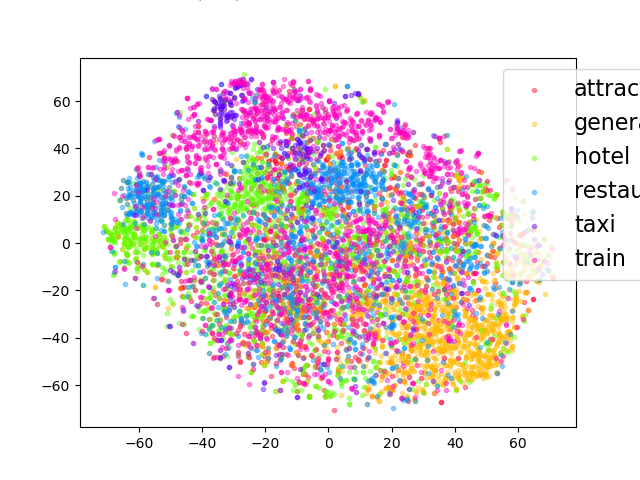
\includegraphics[width=.5\textwidth]{images/lava-tsne/ae-lvl-1-bce.png}}\\

\subfloat[level 3]{\label{sfig:a2}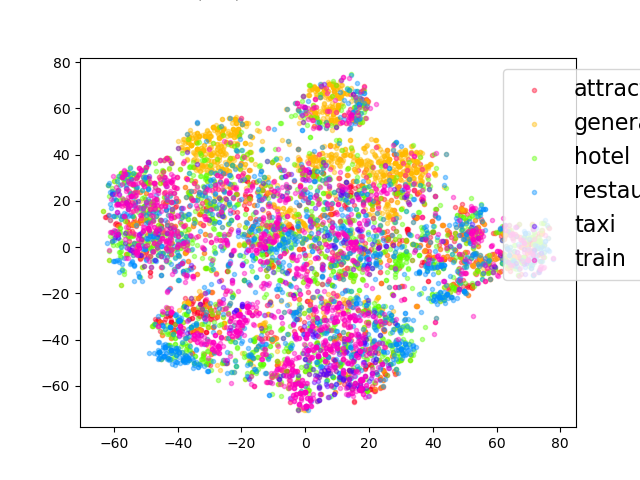
\includegraphics[width=.5\textwidth]{images/lava-tsne/ae-lvl-2-nll.png}}\hfill
\subfloat[level 3 + ph loss]{\label{sfig:b2}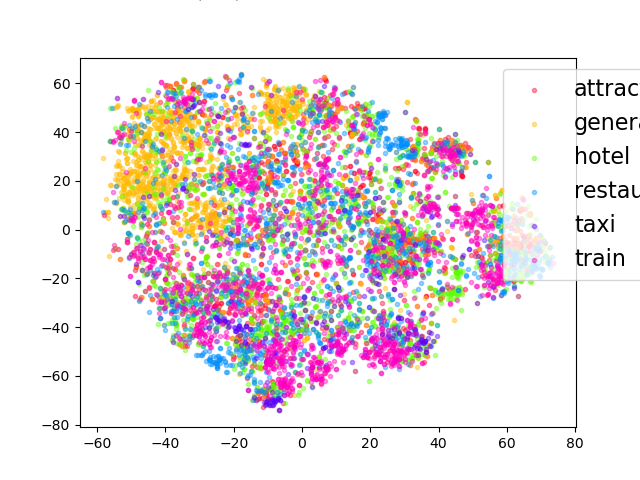
\includegraphics[width=.5\textwidth]{images/lava-tsne/ae-lvl-2-bce.png}}\\
\caption{Visualization of t-SNE projections of latent variables after the autoencoding stage, sorted left-to-right. In the bottom row, we have a version using the additional placeholder loss. The colors correspond to respective domains.}
\label{05:fig:ae-layers}
\end{figure}

\begin{figure}[h]
\centering
\subfloat[level 1]{\label{sfig:c0}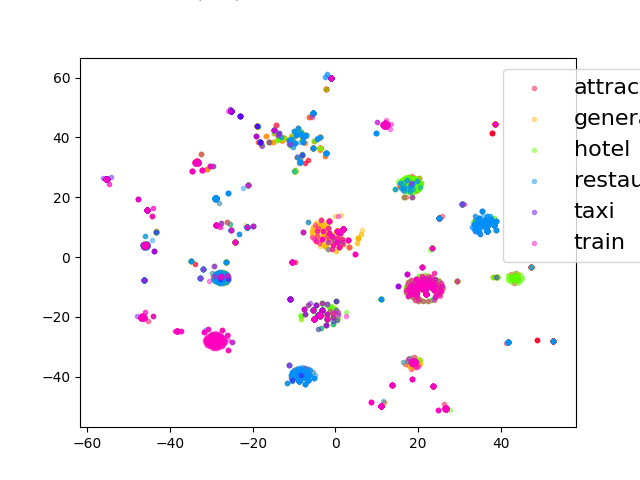
\includegraphics[width=.5\textwidth]{images/lava-tsne/ft-lvl-0-nll.png}}\hfill
\subfloat[level 1 + ph loss]{\label{sfig:d0}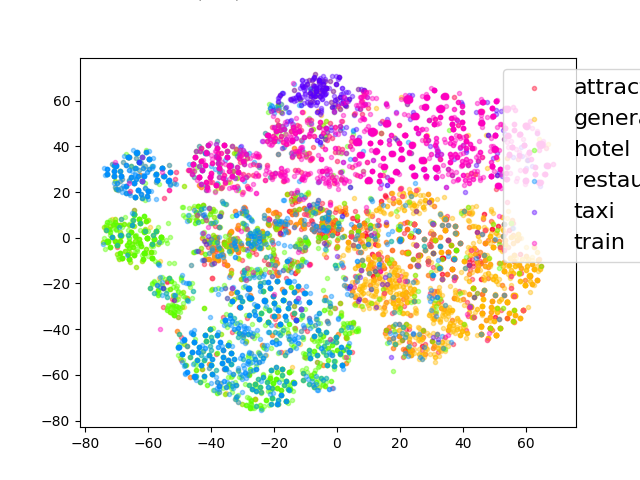
\includegraphics[width=.5\textwidth]{images/lava-tsne/ft-lvl-0-bce.png}}\\

\subfloat[level 2]{\label{sfig:c1}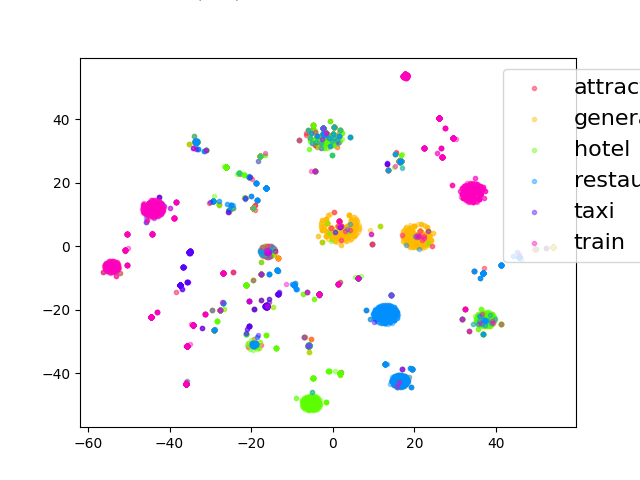
\includegraphics[width=.5\textwidth]{images/lava-tsne/ft-lvl-1-nll.png}}\hfill
\subfloat[level 2 + ph loss]{\label{sfig:d1}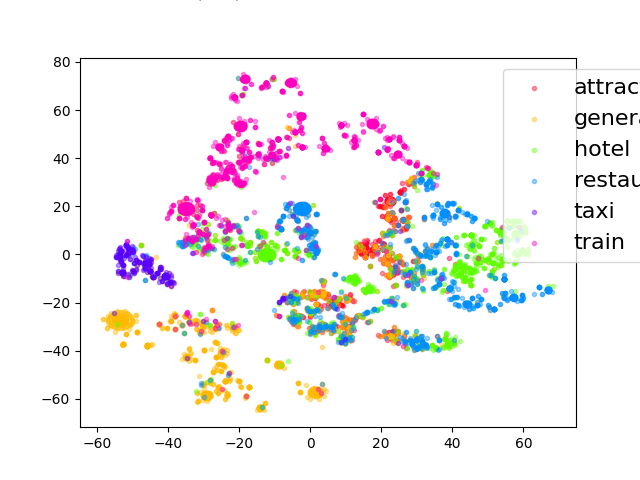
\includegraphics[width=.5\textwidth]{images/lava-tsne/ft-lvl-1-bce.png}}\\

\subfloat[level 3]{\label{sfig:c2}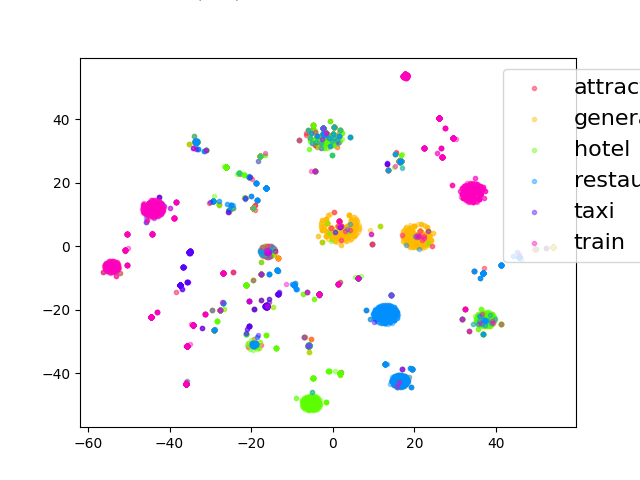
\includegraphics[width=.5\textwidth]{images/lava-tsne/ft-lvl-2-nll.png}}\hfill
\subfloat[level 3 + ph loss]{\label{sfig:d2}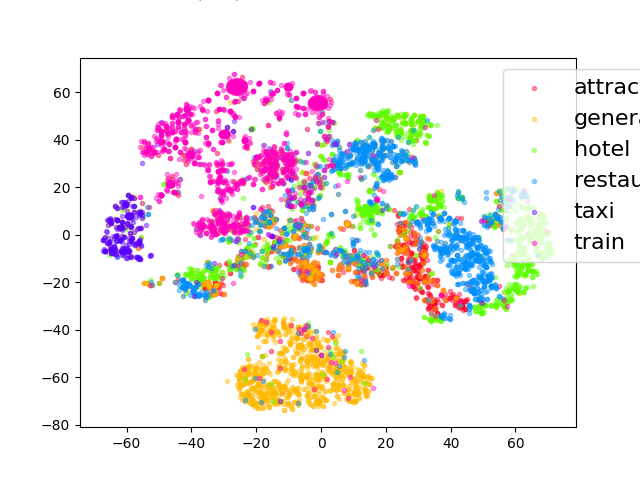
\includegraphics[width=.5\textwidth]{images/lava-tsne/ft-lvl-2-bce.png}}\\
\caption{Visualization of t-SNE projections of latent variables after training for unsupervised dialogue response generation, sorted left-to-right. In the bottom row, we have a version using the additional placeholder loss. The colors correspond to respective domains.}
\label{05:fig:ft-layers}
\end{figure}

\subsection{Conclusion}
In this section, we introduced HVTOD, a hierarchical variational model for task-oriented dialogue.
We wanted to assess the contributions of hierarchical structure to the overall model performance.
Although the layer representations are not guaranteed to be distinct, we show that the model can leverage the benefits introduced by hierarchical structure since the variant with more layers outperforms the baseline (1-layer) variant with the same number of parameters.
The visualizations of latent spaces also uncover that the learned representations are structurally different.
%%%%%%%%%%%%%%%%%%%%%%%%%%%%%%%%%%%%%%%%%%%%%%%%%%%%%%%%%%%%%%%%%%%%%%%%%%%%%
\chapter{Sequence-to-Sequence Task-Oriented Dialogue Modeling}
\label{06:chap:lm-tod}
%%%%%%%%%%%%%%%%%%%%%%%%%%%%%%%%%%%%%%%%%%%%%%%%%%%%%%%%%%%%%%%%%%%%%%%%%%%%%
Using end-to-end trainable models instead of modular architectures (see Section~\ref{02:sec:basics}) can address transferring the learned behavior since we use only a single step and, therefore, can be adjusted to different domains and use cases more easily.
In task-oriented dialogue, end-to-end implementations are dominated by sequence-to-sequence architectures based on language models (LM, Section~\ref{relwork:end-to-end}).
The LM-based approaches have taken over the benchmarks, \footnote{\url{https://github.com/budzianowski/multiwoz\#trophy-benchmarks}}demonstrating state-of-the-art performance.
However, these competitive models are fine-tuned on a single training set.
In this chapter, we raise the question of how well these models can transfer the obtained skill of leading the dialogue to other domains.
In other words, we want to discover if the models learn useful skills that can be beneficial in other domains or if the demonstrated behavior merely reproduces the patterns seen in the training portion of the data.
We hypothesize that pre-training of these models can help to improve the performance.
To confirm this hypothesis, we first describe our approach to end-to-end modeling with the AuGPT model \cite{kulhanek-etal-2021-augpt} in Section~\ref{06:augpt}.
We then describe our data in Section~\ref{06:sec:diaser} and conduct experiments (see Section~\ref{06:expe}).

The work presented in this chapter was published at the LREC conference and covered by~\citet{hudecek-etal-2022-unifying}.
\footnote{This was a joint effort in which we focused on the data preparation pipelines and AuGPT model training.}
For modeling, we use the AuGPT model \cite{kulhanek-etal-2021-augpt} to the development we contributed to during this work.
The experiments published in \citet{hudecek-etal-2022-unifying} are further extended to determine if the model can learn from smaller training sets (\ref{tab:exp-results-seed}).

\section{AuGPT Model Description}
\label{06:augpt}
We choose the AuGPT model introduced by \citet{kulhanek-etal-2021-augpt}.
The architecture utilizes the GPT-2 model~\cite{radford2019language} for both belief state prediction and response generation, following the two-step method described in Section~\ref{background:2stage-lm-modeling}.
GPT-2 is a pre-trained language model based on a Transformer decoder.
Therefore, it is suitable for modeling sequences in natural language.
When evaluated with automatic measures, the model performs well, and it showed promising behavior in human-judged interactive evaluation during the DSTC 9 \citep{gunasekara2020overview} challenge. 
AuGPT directly builds on the \emph{small} version of the model, resulting in a 124M parameter model.
Additionally, AuGPT introduces multiple training improvements.
Instead of solely using cross-entropy loss for language modeling, AuGPT uses an additional training objective for state corruption detection.
During training, the model is randomly presented with corrupted versions of the belief state~\citep{peng2021soloist}.
For corruption, portions of the belief state are replaced with random values.
Several strategies can be used to create the corrupted versions; AuGPT corrupts half of the samples by randomly applying one or more of the following modifications:
\begin{itemize}
    \item Replace the belief state $b$ with another belief state, sampled uniformly randomly from the training data.
    \item Replace the delexicalized response $\bar{r}$ with a different randomly chosen one. If this change is combined with the first one, the delexicalized response and the belief state are taken from the same random sample.
    \item A different valid value is uniformly sampled for each slot in the belief state. In this case, the domain names and order are unchanged (i.e., the active domain is the same).
\end{itemize}
The model learns to predict if the presented belief state corresponds to the respective context in the training example.
This modification aims to improve the robustness of the belief state prediction.
Since GPT can work with any natural language sentences, applying this model to our dialogue datasets is straightforward.

\section{Diaser corpus introduction}
\label{06:sec:diaser}
Motivated by the questions raised in this chapter, we created a collection of several well-established task-oriented dialogue datasets spanning several domains to yield one larger multi-domain corpus which we call \emph{Diaser}.
Specifically, we used: \textbf{MultiWOZ 2.2} (MultiWOZ), \textbf{Schema-guided dialogue} (SGD), \textbf{DSTC2} (DSTC) and \textbf{CamRest676} (CamRest).
For more details about the aforementioned datasets, please refer to Section~\ref{02:sec:input-data-desc}.
The merging process yields a dataset with over 37,000 dialogues, comprising more than 660,000 turns.

\subsection{Theoretical motivation}
We aim to cover as many domains as possible in a unified corpus.
Our source dataset choice is thus mainly based on the level of annotation available -- all source datasets include semantic annotation on the turn level and explicit database interaction. 
Despite the dataset similarities, important differences need to be resolved.

The main task when merging datasets is to unify the different domain-specific ontologies, i.e., the different sets of concepts included in the dialogue acts.
More precisely, the unified dataset ontology contains all the possible domains with corresponding slots and associated value sets.
We cannot consider the slots independently from the domain they belong to.
Indeed, a slot that represents the \textit{price range} will not have the same range of values when relating to a restaurant or a flight ticket.
We identified two main problems related to this issue:
\begin{enumerate}
    \item \textbf{Name reference ambiguities}
    We must design the final ontology so that different slot names refer to different concepts (with due precaution for label choice) and merge different slot names associated with the same value set under a single label.
    For example, in MultiWOZ, there are two different slot names \textit{day} and \textit{book-day} for the same value set (weekdays) and usage contexts.
    But in SGD, these slot names may be misleading since we can find a slot named \textit{start-day} and another called \textit{day}; the former refers to a calendar date while the latter refers to a weekday.
    
    \item \textbf{Absence of ontology/database} When the SGD dataset was collected, the authors used API calls instead of a database lookup.
    They also didn't provide an overall ontology.
    Therefore, no database-related metadata was released with the corpus, forcing us to create an ontology and a database for the data based on values occurring in the conversations.
\end{enumerate}

\subsection{Details of the merging approach}
\begin{table}[tp]
    \centering\footnotesize
    \begin{tabular}{l@{\hspace{0.8em}}r@{\hspace{0.3em}}r@{\hspace{0.3em}}r@{\hspace{0.3em}}r@{\hspace{2em}}r}
        \toprule
        \textbf{Data}         & \textbf{SGD} & \textbf{MultiWOZ} & \textbf{DSTC} & \textbf{CamRest} & \textbf{Total} \\ \midrule
        \textbf{Domains}        & 18        &    7        &      1        &      1      &    19$^{\ast}$ \\
        \textbf{Slots}        & 145       &    29       &     10        &      7      & 166$^{\ast}$ \\
        \textbf{Dialogues$^{\ast\ast}$}       & 22.8    & 10.4     &    3.2     &      0.7   & 37.1\\
        \textbf{Turns$^{\ast\ast}$}        & 463.3   & 143.0     &    51.0  &     5.5   & 662.8\\
        \textbf{Turns/Dial.}   & 20.30     & 13.71       &   15.77        &     8.12    & 17.83 \\
        \textbf{Avg. utt. length} & 9.86      &  13.23      &   8.47        &  10.71       & 10.49 \\
        \textbf{Unique Words}$^{\ast\ast}$ & 32.3 & 23.2 & 1.3 & 1.7 & 49.9 \\
        \textbf{Shannon ent.} & 8.96 & 8.54 & 7.04 & 7.69 & 9.01 \\
        \textbf{Cond. ent.} & 4.76 & 4.41 & 2.14 & 2.95 & 4.83 \\

     \bottomrule
    \end{tabular}
    \caption{Composition of our dataset, with basic statistics, overall and for individual sources (number of domains and slots, total numbers of dialogues and turns, average number of turns per dialogue, and average utterance length in terms of words. $^{\ast}$ is not a sum due to ontology merging. $^{\ast\ast}$ in thousands.}
    \label{06:tab:final_data_stats}
\end{table}
Here, we present details on how we merged the data into a common format, including handling different ontologies.
Quantitative statistics of the final dataset are shown in Table~\ref{06:tab:final_data_stats}.
Full technical documentation can be found in the data repository.\footnote{\url{https://github.com/ufal/diaser}}
Here we list an overview of all the required merging steps:

\paragraph{Matching belief representations.} In DSTC and CamRest, belief state annotations are extracted from the user and the system utterance.
In contrast, in the MultiWOZ and SGD datasets, the belief state is only extracted from the user utterance.
We had to filter automatically the annotations from DSTC and CamRest until they matched the MultiWOZ belief state representation. 
    
\paragraph{Adding meta features} from the original datasets. DSTC2, CamRest, and MultiWOZ contain the \emph{goal} of the dialogue (also called task) as a dialogue act with the constraints (e.g. expensive restaurant south) and the information the user needs to obtain from the system (e.g. phone number and address). They also contain a short text summarizing this goal for crowd workers. We include both versions of the task description with each dialogue.
    
\paragraph{Unifying annotation structure.} The final dataset structure is similar to the structure of SGD and MultiWOZ 2.2. We create a \textit{Turn} object that contains either the user utterance and dialogue acts or the system utterance.
Two consecutive entries for the user and system share the same turn number -- we consider a \textit{Turn} as an exchange between the user and the system (i.e. a pair or utterances). 

\paragraph{Ontology unification.}   
One of the most difficult parts of this work was unifying the ontologies of each original dataset because they were not built on the same dimensions.
This concerns slot, domain, and intent names.

After indexing all annotations from the different datasets, we merged them manually using MultiWOZ as a golden reference to create the mapping.
We always check the meaning in context and match slots/intents with the same semantics.

% In addition to unifying the naming, we also needed to address that the ontologies distinguish between two kinds of slots: informable and requestable (see Section\ref{02:ds-background}).We use this distinction to also assign slots in the other two datasets into one of these two groups.

\paragraph{Slot co-reference}
Some source corpora (MultiWOZ and SGD) include co-reference between slots.
For example, \textit{start-time} can take the value “sooner than that” or the slot \emph{hotel-name} can take the value “event you mentioned earlier”.
This is a problem if we assume a self-contained ontology that captures all the possible values from the corpus.
However, as these co-references are impossible to include in the ontology easily, we leave these values unchanged and the slot co-references are carried over to the unified data.

\begin{table}[tp]
    \centering\footnotesize
    \begin{tabular}{l>{\hspace{-3mm}}r>{\hspace{-2mm}}rrr>{\hspace{-2mm}}r}
        \toprule
        \bf Intent &
        \textbf{SGD} & 
        \textbf{MultiWOZ} &
        \textbf{DSTC} &
        \textbf{CamRest} &
         \textbf{all}\\ \midrule
        \textbf{inform} & 151,467 & 84,259 & 33,451 & 5,786 & 274,963\\ 
        \textbf{request} & 81,786 & 31,888 & 13,620 & 1,516 & 128,810\\ 
        \textbf{offer} & 67,095 & 4,497 & 23,763 & 0 & 95,355\\ 
        \textbf{bye} & 35,089 & 12,380 & 0 & 0 & 47,469\\ 
        \textbf{else}& 31,030 & 13,779 & 0 & 0 & 44,809 \\ 
        \textbf{select}& 33,820 & 2,834 & 243 & 0 & 36,897\\ 
        \textbf{confirm}& 30,327 & 0 & 5,756 & 0 & 36,083\\
        \textbf{thank}& 23,172 & 9,064 & 0 & 0 & 32,326\\ 
        \textbf{negate}& 132,01 & 4,399 & 4,413 & 0 & 22,023\\ 
        \midrule
        \textbf{total}& 435,957 & 163,100 & 81,346 & 7,312 & 718,645\\
        \bottomrule
    \end{tabular}
    \caption{Most frequent intents in our unified schema, for each source dataset individually and overall (with absolute numbers of occurrences).}
    \label{tab:intents}
\end{table}

\begin{table}[tp]
    \centering\footnotesize
    \begin{tabular}{l>{\hspace{-2mm}}rrrrr}
        \toprule
        \bf Slot &
        \textbf{SGD} & 
        \textbf{MultiWOZ} &
        \textbf{DSTC} &
        \textbf{CamRest} &
         \textbf{all}\\ \midrule
        \textbf{name} & 65,999 & 42,215 & 3,135 & 2 & 111,351\\ 
        \textbf{area} & 8,133 & 48,285 & 37,697 & 4,178 & 98,293 \\ 
        \textbf{date} & 81,600 & 20,872 & 0 & 0 & 102,472\\
        \textbf{price} & 1,950 & 33,084 & 32,267 & 4,032 & 71,333\\
        \textbf{type}& 41,146 & 28,562 & 0 & 0 & 69,708\\
        \textbf{leave}& 32,625 & 26,684 & 0 & 0 & 59,309\\
        \textbf{arrive}& 26,180 & 26,228 & 0 & 0 & 52,408\\
        \textbf{food}& 13,501 & 20,963 & 3,007 & 571 & 38,042\\
        \textbf{book}& 17,618 & 11,723 & 0 & 0 & 29,341\\
        \midrule
        \textbf{total}& 298,752 & 232,388 & 76,106 & 8,783 & 532,257\\
        \bottomrule
    \end{tabular}
    \caption{Most frequent slots in our unified schema, for each source dataset individually and overall (with absolute numbers of occurrences).}
    \label{tab:slots}
\end{table}

\section{Experiments}
\label{06:expe}

In this chapter, we want to explore if sequence-to-sequence LM-based architectures can robustly learn the dialogue modeling capabilities and how well they can transfer them to other domains.
To answer these questions, we conduct a series of experiments to train the model using only a small portion of the training data or even a different dataset with shared characteristics such as a task-oriented approach, regular user-system interaction, etc.

We divide the results into two sections.
First, we describe the performance of the AuGPT model when trained and evaluated on various datasets.
In the second section, we show the results when the model is pre-trained on a certain dataset and then fine-tuned using only a small portion of training data from the target dataset.

We are interested in the overall performance of the models.
Therefore, we measure Joint Goal Accuracy and Slot-F1 and BLEU for response generation (see Section~\ref{02:sec:eval_metrics}).
We do not compute the dialogue success as it is not well-defined on all the sub-datasets.

\subsection{Exerimental setup}
For training, we follow~\citep{kulhanek-etal-2021-augpt} with the training setup --
We use PyTorch framework \cite{pytorch} and run the training for 8 epochs on the MultiWOZ data when all the training examples are used.
The AuGPT model described in Section~\ref{06:augpt} consists of 12 transformer blocks with a model layer size equal to 768, having 124 million parameters in total.
For the state corruption detection task, we use a dropout of 0.1 with label smoothing of 0.1.
We use the AdamW optimizer \cite{DBLP:conf/iclr/LoshchilovH19} and employ mixed-precision training \cite{micikevicius2017mixed}.

For the data, we follow the dataset discussed in Section~\ref{06:sec:diaser}.
We use different subsets for training and testing the model, as described for each experiment individually.

\subsection{Influence of training data on the target performance}
\begin{table*}[tp]
    \centering \small
    \begin{tabular}{ccc >{\hspace{1em}} ccc >{\hspace{1em}} ccc}
      \toprule
       \multicolumn{3}{c}{training} & \multicolumn{3}{c}{evaluation} & \multicolumn{3}{c}{metrics}\\
       \textbf{DSTC} & \textbf{MW} & \textbf{SGD} & \textbf{DSTC} & \textbf{MW} & \textbf{SGD} & \textbf{Slot F1} & \textbf{JGA} & \textbf{BLEU} \\
       %========================================================
       \midrule
       %========================================================
       % mwoz-mwoz
       {\textcolor{red} \xmark} & {\textcolor{green} \cmark} & {\textcolor{red} \xmark} & {\textcolor{red} \xmark} & {\textcolor{green} \cmark} & {\textcolor{red} \xmark} & 0.89 & 0.53 & 18.61 \\
       % schema-mwoz
       {\textcolor{red} \xmark} & {\textcolor{red} \xmark} & {\textcolor{green} \cmark} & {\textcolor{red} \xmark}  & {\textcolor{green} \cmark} & {\textcolor{red} \xmark} & 0.16 & 0.02 & 4.01 \\
       % dsctmwoz-mwoz
       {\textcolor{green} \cmark} & {\textcolor{green} \cmark} & {\textcolor{red} \xmark} & {\textcolor{red} \xmark}  & {\textcolor{green} \cmark} & {\textcolor{red} \xmark} & 0.89 & {0.55} & 19.67 \\
       % dstcschema-mwoz
       {\textcolor{green} \cmark} & {\textcolor{red} \xmark} & {\textcolor{green} \cmark} & {\textcolor{red} \xmark}  & {\textcolor{green} \cmark} & {\textcolor{red} \xmark} & 0.17 & 0.03 & 5.68 \\
       % mwozschema-mwoz
       {\textcolor{red} \xmark} & {\textcolor{green} \cmark} & {\textcolor{green} \cmark} & {\textcolor{red} \xmark}  & {\textcolor{green} \cmark} & {\textcolor{red} \xmark} & 0.89 & 0.52 & 19.92 \\
       % all-mwoz
       {\textcolor{green} \cmark} & {\textcolor{green} \cmark} & {\textcolor{green} \cmark} & {\textcolor{red} \xmark}  & {\textcolor{green} \cmark} & {\textcolor{red} \xmark} &  0.90 & 0.54 & 21.09 \\
       %========================================================
       \midrule
       %========================================================
       % mwoz-schema
       {\textcolor{red} \xmark} & {\textcolor{green} \cmark} & {\textcolor{red} \xmark} & {\textcolor{red} \xmark} & {\textcolor{red} \xmark} & {\textcolor{green} \cmark} & 0.04 & 0.01 & 5.63 \\
       % schema-schema
       {\textcolor{red} \xmark} & {\textcolor{red} \xmark} & {\textcolor{green} \cmark} & {\textcolor{red} \xmark}  & {\textcolor{red} \xmark} & {\textcolor{green} \cmark} & 0.59 & 0.21 & {28.17} \\
       % dstcmwoz-schema
       {\textcolor{green} \cmark} & {\textcolor{green} \cmark} & {\textcolor{red} \xmark} & {\textcolor{red} \xmark}  & {\textcolor{red} \xmark} & {\textcolor{green} \cmark} & 0.03 & 0.01 & 5.51 \\
       % dstcschema-schema
       {\textcolor{green} \cmark} & {\textcolor{red} \xmark} & {\textcolor{green} \cmark} & {\textcolor{red} \xmark}  & {\textcolor{red} \xmark} & {\textcolor{green} \cmark} & 0.58 & 0.21 & 27.96 \\
       % mwozschema-schema
       {\textcolor{red} \xmark} & {\textcolor{green} \cmark} & {\textcolor{green} \cmark} & {\textcolor{red} \xmark}  & {\textcolor{red} \xmark} & {\textcolor{green} \cmark} & 0.63 & 0.23 & 27.54 \\
       % all-schema
       {\textcolor{green} \cmark} & {\textcolor{green} \cmark} & {\textcolor{green} \cmark} & {\textcolor{red} \xmark}  & {\textcolor{red} \xmark} & {\textcolor{green} \cmark} & 0.63 & 0.22 & 27.72 \\
       %========================================================
       \midrule
       %========================================================
       % dstcmwoz-all
       {\textcolor{green} \cmark} & {\textcolor{green} \cmark} & {\textcolor{red} \xmark} & {\textcolor{green} \cmark} & {\textcolor{green} \cmark} & {\textcolor{green} \cmark} & 0.28 & 0.12 & 15.30 \\
       % dstcschema-all
       {\textcolor{green} \cmark} & {\textcolor{red} \xmark} & {\textcolor{green} \cmark} & {\textcolor{green} \cmark} & {\textcolor{green} \cmark} & {\textcolor{green} \cmark} &  0.55 & 0.22 & 27.28 \\
       % mwozschema-all
       {\textcolor{red} \xmark} & {\textcolor{green} \cmark} & {\textcolor{green} \cmark} & {\textcolor{green} \cmark} & {\textcolor{green} \cmark} & {\textcolor{green} \cmark} & 0.65 & 0.25 & 25.13 \\
       % all-all
       {\textcolor{green} \cmark} & {\textcolor{green} \cmark} & {\textcolor{green} \cmark} & {\textcolor{green} \cmark} & {\textcolor{green} \cmark} & {\textcolor{green} \cmark} & 0.70 & 0.28 & \textbf{29.73} \\

      \bottomrule
  \end{tabular}
  \caption{Performance of the AuGPT model trained and evaluated on various subsets of the unified dataset, namely DSTC, MultiWOZ (MW), and SGD. We omit CamRest since the data are very similar to DSTC.}
  \label{06:tab:exp-results-diaser}
\end{table*}

In Table~\ref{06:tab:exp-results-diaser}, we can see a general pattern in the results, suggesting that the model fails to generalize across different datasets when a subset of data we evaluate is not included in the training. A significant drop in performance can be observed across all recorded metrics.
We use  DSTC, MultiWOZ (MW), and SGD. We omit CamRest since the data are very similar to DSTC.

Let us first observe some global properties.
Regarding the $F_1$ slot score and joint goal accuracy, the explanation for the poor model's accuracy can be found in a substantially different distribution of slots across SGD/MultiWOZ datasets and DSTC.
Some slots are present in just one of the datasets, others are mentioned in different contexts or with different frequencies.
Training on MultiWOZ provides us with the highest scores on slot $F_1$ and joint goal accuracy.
Training on both SGD and MultiWOZ brings only a very marginal improvement.
The large difference in performance can also be seen in terms of BLEU, which suggests a vastly different language used in each dataset.

The performance of the model evaluated on MultiWOZ is analogous.
Training the model solely on SGD gives us a model that cannot generalize to MultiWOZ data.
Concatenating the MultiWOZ datasets with SGD/DSTC, or both during training, leads to a little improvement, predominantly in terms of BLEU score.
We get the best results when using all three datasets for training and obtain the model with better generalizing capabilities supported by the BLEU score of 21.09.

The model evaluation on SGD data mostly follows the same pattern. However, in this case, it is quite interesting to observe that training the model on all three datasets is not beneficial, and the performance stagnates, although the training set is much larger.

Finally, if we evaluate all three datasets, it is clear that the best-performing model is obtained when we train it on the full data.
Table \ref{tab:exp-results-diaser} shows that including SGD data is crucial for achieving higher BLEU values while training on MultiWOZ helps the model predict slot values.

\subsection{Domain adaptation with a small in-domain set}
Table~\ref{tab:exp-results-seed} presents results for domain adaptation experiments.
We first train the AuGPT model on the MultiWOZ dataset and then use a small portion of the SGD data to adapt the model to this different dataset.
The results show that although on MultiWOZ helps slightly to improve the final BLEU score, the performance of belief state tracking is not significantly improved, and the results are overall rather negative.

\begin{table*}[tp]
    \centering \small
    \begin{tabular}{cccccc}
      \toprule
       pre-training & fine-tuning & ft-ratio & \textbf{Slot-F1} & \textbf{JGA} & \textbf{BLEU} \\
        \midrule
       -- & SGD & 100\% & 0.59 & 0.21 & 28.17 \\
       -- & SGD & 10\% & 0.47 & 0.15 & 20.13 \\
       MultiWOZ & SGD & 10\% & 0.46 & 0.16 & 19.46 \\
       -- & SGD & 5\% & 0.29 & 0.08 & 14.65 \\
       MultiWOZ & SGD & 5\% & 0.29 & 0.12 & 15.16 \\
       -- & SGD & 1\% & 0.07 & 0.03 & 6.37\\
       MultiWOZ & SGD & 1\% & 0.06 & 0.01 & 8.40 \\
       -- & SGD & 0.5\% & 0.04 & 0.04 & 3.43 \\
       MultiWOZ & SGD & 0.5\% & 0.04 & 0.02 & 5.95 \\
       %========================================================
       \midrule
       %=======================================================
      \bottomrule
  \end{tabular}
  \caption{Performance of the AuGPT model trained and evaluated on various subsets of the unified dataset.}
  \label{tab:exp-results-seed}
\end{table*}


\subsection{Dynamics of Successful and Failed Dialogues}
We also perform a detailed quantitative analysis of errors made by the trained models.
We evaluated the AuGPT model trained on the MultiWOZ data with respect to the dialogue success rates.
We only chose the MultiWOZ data due to the additional annotation available in MultiWOZ.
Specifically, MultiWOZ also has user and system dialogues act annotated, which we use in this analysis.
We consider dialogue success as defined in Section~\ref{02:sec:eval_metrics}.

In Figure~\ref{fig:error_distr}, we provide a histogram of dialogue state tracking errors in successful and failed dialogues.
We further identify four reasons that can cause an error:
\begin{enumerate}
    \item A \emph{domain} is wrongly identified.
    \item An \emph{intent} is detected wrongly.
    \item An \emph{inform} value is captured incorrectly.
    \item A \emph{request} was not answered.
\end{enumerate}
We go turn by turn and identify the errors in the dialogue state predicted by the system compared to the expected state.
``All failed" and ``all success" correspond to failed and successful dialogues.
It is thus an evaluation concerning the dialogue as a whole, unlike the turn-level methods, such as evaluating the system's response generation.
In particular, we show the count of cases where some information is understood wrongly by the system (positive values) or is missing completely (negative values).
We can see that in successful dialogues, the system might make some mistakes at first but can recover eventually.
On the other hand, most dialogue failures are caused by missing information in the second half of the dialogue, which suggests that the recovery is not certain.

We made some observations:
\begin{itemize}
    \item For both successful and unsuccessful dialogues, the first turn concentrates the most errors.
    
    \item Generally speaking, the failed dialogues show much superfluous information in the first five speech turns, especially regarding the user's intent. On the other hand, from approximately the fourth speech turn onwards, there is a lot of missing information, especially at the level of the dialogue domain. If we add the missing information with the superfluous information, the error distribution peaks between turns three and seven of the dialogue. 
\end{itemize}

\begin{figure}[tp]
    \centering  \small
    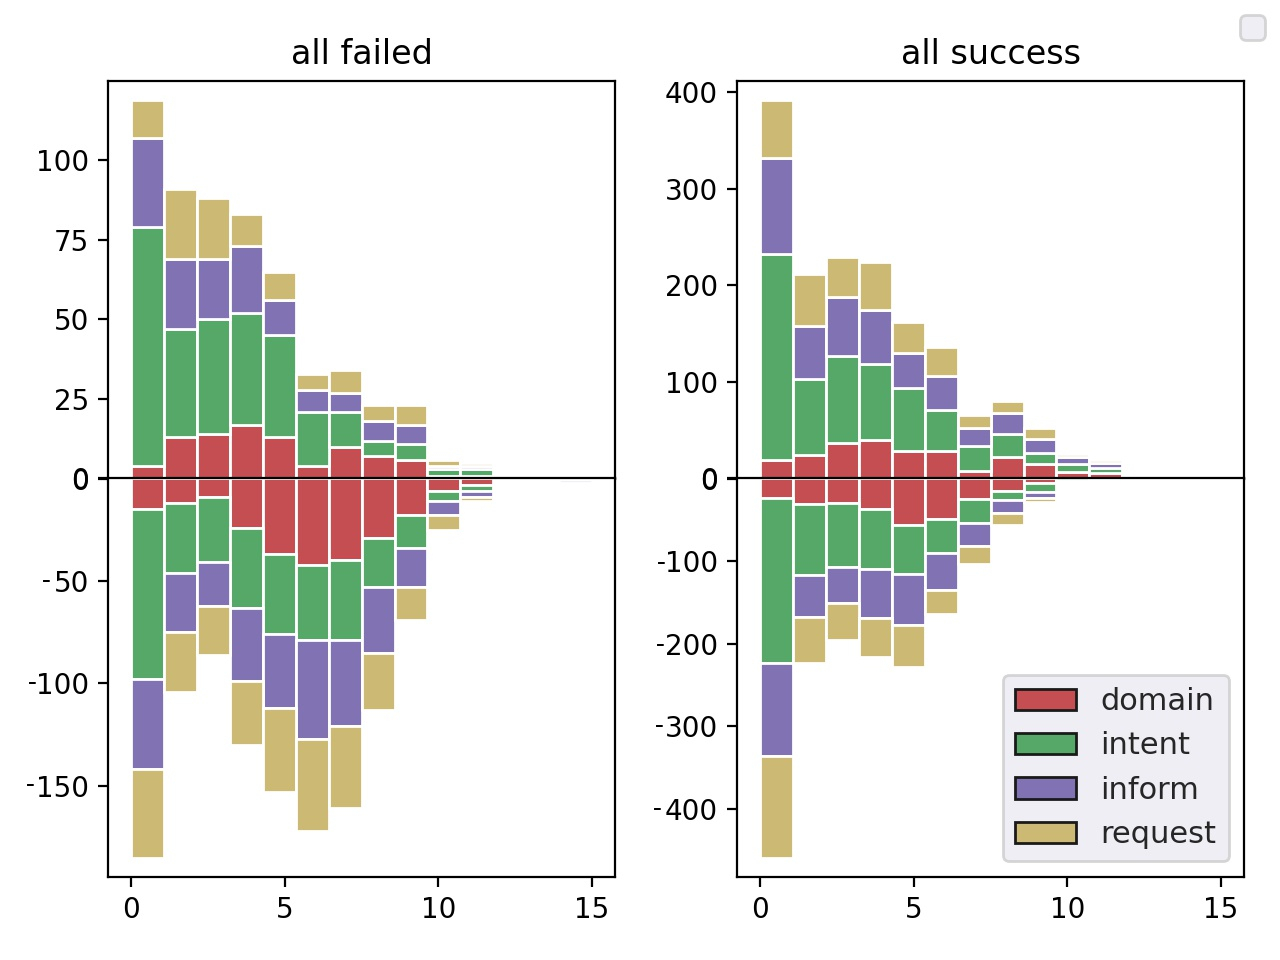
\includegraphics[width=0.49\textwidth]{images/hist-vert-True-gpt.jpg}
    \caption{Distribution and types of dialogue failures that occurred with the GPT2-based model on the MultiWOZ data.
    The horizontal axis corresponds to turn numbers. Positive values represent cases where the information is captured wrongly, while negative values represent cases where particular information is missing.
    The source of error (incorrect domain or intent, missing information, or not providing a request) is depicted as color-coded.}
    \label{fig:error_distr}
\end{figure}



\section{Conclusion}
In this work, we unified a large task-oriented dialogue corpora at both data and annotation levels, which requires a complex process of merging ontologies. 
We showed that additional data from other sources helps train LM-based end-to-end dialogue models when converted to a unified format in specific cases.
However, it is not a general rule.
Although the new dataset is still far from perfect coverage, it is a step towards wider and more authentic data.
We also performed experiments to explore the ability of LM-based systems to adapt to new domains easily with a small number of in-domain examples.
The negative results suggest that using in-domain data for domain adaptation is not straightforward.
%%%%%%%%%%%%%%%%%%%%%%%%%%%%%%%%%%%%%%%%%%%%%%%%%%%%%%%%%%%%%%%%%%%%%%%%%%%%
\chapter{Large Language Models for Task-Oriented Dialogue}
\label{chap:llms}
%%%%%%%%%%%%%%%%%%%%%%%%%%%%%%%%%%%%%%%%%%%%%%%%%%%%%%%%%%%%%%%%%%%%%%%%%%%%

\label{07:sec:intro}
As described in the previous chapter, pre-trained Language Models perform very well in end-to-end dialogue modeling.
Despite this success, the widely used approach of fine-tuning pre-trained LM on a particular dataset still does not guarantee easy transferability of the learned knowledge.
Large Language Models (LLMs) increased the model size by an order of magnitude compared to the previous generation of pre-trained LMs.
Undeniably, LLMs have transformed the NLP field,
showing outstanding performance across many NLP benchmarks such as Winograd Challenge \cite{levesque2012winograd} or GLUE \cite{wang2018glue}.
Instruction fine-tuning of LLMs can align the model outputs with human preferences \cite{ouyang2022training,supernaturalinstructions} and improve the LLMs' communication capabilities substantially.

State-of-the-art LLMs are good at understanding user needs and can provide relevant answers.
Consequently, we have seen many chatbot applications both inside and outside academia (ChatGPT\footnote{\url{https://openai.com/blog/chatgpt}}, Claude\footnote{\url{https://www.anthropic.com/index/introducing-claude}} or Bard\footnote{\url{https://blog.google/technology/ai/bard-google-ai-search-updates/}}) which build upon the raw power of instruction-fine-tuned LLMs.

In this chapter, we explore the abilities of LLM to model task-oriented dialogue using in-context learning.
We evaluate the performance regarding response generation and dialogue success.
To obtain more insights, we also perform a human evaluation to test more real-world scenarios.
We introduce an LLM-based TOD conversation pipeline and evaluate its performance concerning commonly used task-oriented metrics such as Joint Goal Accuracy, Slot F1, and Dialogue Success \cite{rastogi_multi-task_2018,budzianowski_multiwoz_2018}, see also Section~\ref{02:sec:eval_metrics}.
Our pipeline resembles other approaches based on LMs \cite{peng-etal-2021-soloist,yang2021ubar}, using state tracking and response generation as two main, separate steps while keeping the role of a dialogue policy implicit (see also Sections~\ref{background:2stage-lm-modeling},\ref{06:augpt}).
However, instead of fine-tuning LMs, it intentionally relies almost exclusively on using pre-trained LLMs as-is so we can test their out-of-the-box capabilities.
The dialogue context and domain description are introduced to the model only by including them in the input prompt.
We experiment with zero-shot and few-shot approaches (see Section~\ref{02:in-context}).
In the zero-shot setting, the model receives a domain description only; in the few-shot setting, it additionally uses a few retrieved examples (see Section~\ref{07:sec:method} for details).
This work was published at the SIGDial 2023 conference~\cite{hudecek-dusek-2023-large} and was extended in this chapter with more details and additional experiments.

\section{Motivation}
Given the millions of daily interactions with LLM-based chatbots, these models can handle users' needs satisfactorily, at least to some extent.
However, these chatbots are tuned using unstructured open-domain conversations.
We aim to evaluate these systems on task-oriented dialogues, where the system has to follow a predetermined structure and handle external sources of information, such as APIs or databases.
We ask to what extent LLMs can handle these applications off-the-shelf, i.e., without fine-tuning.
This approach, frequently referred to as \emph{in-context learning} or \emph{prompting}, is a common way to work with LLMs and offers competitive performance.
Moreover, TOD systems output in-domain information with a predetermined structure and lend itself well to evaluation, thanks to pre-existing annotated data sets.
We avoid fine-tuning techniques and focus on zero-shot or few-shot settings using in-context learning, as this approach has lower hardware requirements and barrier of entry and better flexibility or even performance in certain tasks \cite{su2022selective}.
It is important to note that we cannot exclude the possibility that some models were exposed to our selected datasets during training~\citep{golchin2023time}.
However, evaluating this setting is important as the real-world use cases might largely rely on this approach.


Our experiments show that LLMs are not very good at state tracking, and their performance falls behind state-of-the-art, task-specific trackers.
However, if provided with correct belief states, some yield interesting response generation performance comparable to earlier fine-tuned state-of-the-art models.
Moreover, our human evaluation experiments show that LLMs are generally good with human interactions, and their performance cannot be assessed only based on automatic evaluations.

\section{Method}
\label{07:sec:method}
\begin{figure}[t]
    \centering
    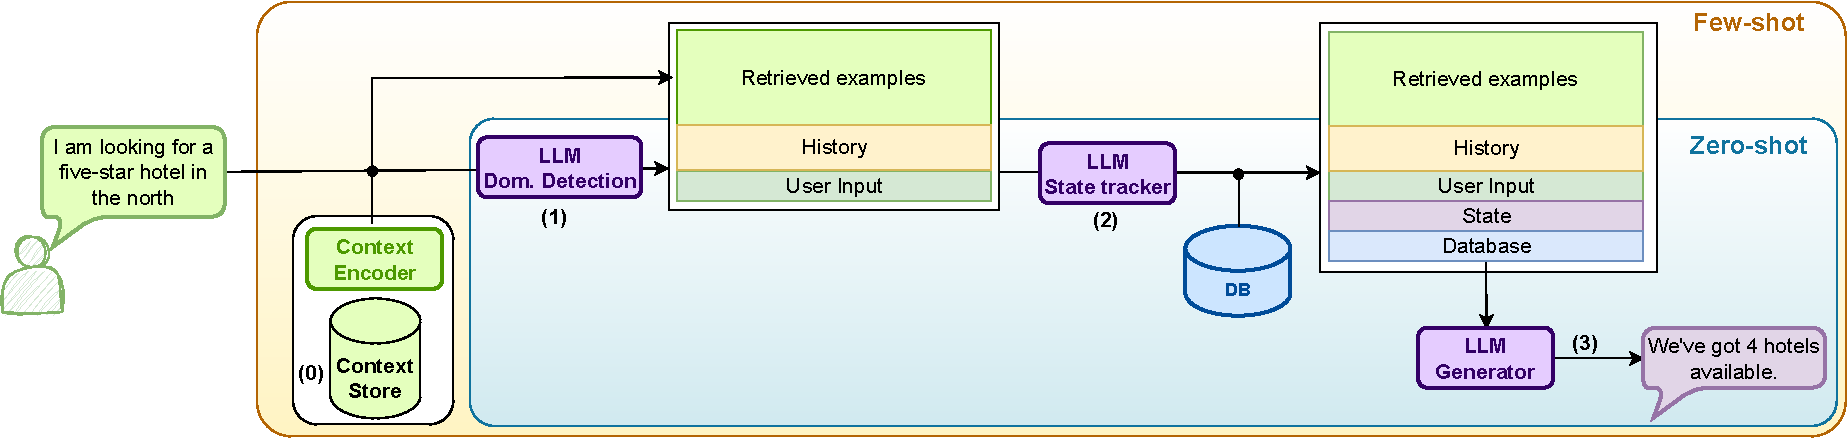
\includegraphics[width=\textwidth]{images/llm-chatbot-v3.pdf}
    \caption{A detailed description of our proposed pipeline. (0) As a preprocessing step, we encode a subset of the training set that will be used to retrieve few-shot examples.
    Given a user input, we: (1) Detect the domain, retrieve relevant examples (in the few-shot setting), and construct an initial prompt. (2) Infer the belief state using LLM. Based on that, we retrieve database information and construct another prompt that includes the state and database results. (3) We ask the LLM to provide a final response.}
    \label{07:fig:overview_low_level}
\end{figure}
An overall description of the proposed pipeline is shown in Figure~\ref{07:fig:overview_low_level}.
The system consists of a pre-trained LLM and an (optional) context store in a vector database.
Three LLM calls are performed in each dialogue turn, with specific prompts (see Section~\ref{07:sec:prompts}).
First, the LLM performs domain detection and state tracking (Section~\ref{07:sec:state-tracking}).
The updated belief state informs a database query, the results of which are used in the subsequent LLM-based response generation step~\ref{07:sec:response}.
In the few-shot setting, the context store stores a limited number of examples from the training set, which are retrieved based on similarity with the conversation context and included in LLM prompts (see Section~\ref{07:sec:context-store}).


\subsection{Prompt construction}
\label{07:sec:prompts}
We aim to compare the raw capabilities of the selected LLMs.
Therefore, we do not focus on prompt engineering techniques and choose universal prompts for all LLMs in this work.
We choose simple, plain language statements as prompts, with no specific vocabulary, based only on a few preliminary tests.
We define a single \textbf{domain detection prompt} (Table~\ref{07_tab:domain}) for all examples, plus a pair of prompts for each domain in the given dataset: a \textbf{state tracking prompt} (Table~\ref{07_tab:zero-shot-state}) and a \textbf{response prompt} (Table~\ref{07_tab:zero-shot-response}).

The domain detection prompt includes a task description and two static examples of domain detection.
In addition to general instructions, each state tracking prompt contains a domain description, a list of relevant slots, the dialogue history, and the current user utterance.
The response prompts do not contain the per-domain slot list but include the current belief state and database results.
In the few-shot setting, each tracking and response prompt contains positive and negative examples retrieved from the context store (see Section~\ref{07:sec:context-store}).

\begin{table}[tp]
    \centering\small
    \begin{tabular}{rl}
      \toprule
      \textbf{Prompt} & \texttt{{\color{cyan!80!yellow!80!black!100 } Determine which domain is considered in the following}}\\
      & \texttt{{\color{cyan!80!yellow!80!black!100 }dialogue situation. }}\\
      & \texttt{ {\color{green!100!yellow!70!black!100 } Choose exactly one domain from this list:}}\\
      & \texttt{ {\color{green!100!yellow!70!black!100 }restaurant, hotel, attraction, taxi, train }} \\
      & \texttt{ {\color{cyan!80!yellow!80!black!100 } Answer with only one word, the selected domain from the list. }}\\
      & \texttt{ {\color{cyan!80!yellow!80!black!100 }You have to always select the most probable domain.}} \\
& \texttt{{\color{red!50!yellow!90!black!100!}  ------- Example 1: -------- }} \\
& \texttt{{\color{red!50!yellow!90!black!100!} Customer: I need a cheap place to eat}} \\
&\texttt{ {\color{red!50!yellow!90!black!100!} Assistant: We have several not expensive places available. }} \\
& \texttt{ {\color{red!50!yellow!90!black!100!}What food are you interested in?}} \\
& \texttt{{\color{red!50!yellow!90!black!100!} Customer: Chinese food.}} \\
& \texttt{{\color{red!50!yellow!90!black!100!}Domain: restaurant}} \\
& \texttt{{\color{red!50!yellow!90!black!100!} ------ Example 2: -------- } }\\
& \texttt{{\color{red!50!yellow!90!black!100!} Customer: What is the address?} } \\
&\texttt{{\color{red!50!yellow!90!black!100!} Assistant: It's 123 Northfolk Road. }} \\
& \texttt{ {\color{red!50!yellow!90!black!100!} Customer: That's all. I also need a train from London. }} \\
&  \texttt{{\color{red!50!yellow!90!black!100!} Domain: train }}\\
& \texttt{{\color{red!50!yellow!90!black!100!} ----------- }} \\
& \texttt{{\color{cyan!80!yellow!80!black!100 } Now complete the following example:}} \\
& \texttt{{\color{orange!50!yellow!90!black!100!} Customer: I am looking for a cheap place to stay. }}\\
& \texttt{Domain:} \\
      \midrule
      \textbf{Output:} & \texttt{hotel} \\
      \bottomrule
  \end{tabular}
    \caption{A prompt used for domain detection for MultiWOZ.
  It contains {\color{cyan!80!yellow!80!black!100} task definition},  {\color{green!100!yellow!70!black!100!}domains description}, {\color{red!50!yellow!90!black!100!} static examples} and {\color{orange!50!yellow!90!black!100!} user utterance}, coded by respective colors.}
  \label{07_tab:domain}
\end{table}

\begin{table}[tp]
    \centering\small
    \begin{tabular}{rl}
      \toprule
      \textbf{Prompt} & \texttt{{\color{cyan!80!yellow!80!black!100 }Definition: Capture entity values from last utterance}}\\
      & \texttt{{\color{cyan!80!yellow!80!black!100 }of the conversation according to examples.}} \\
    & \texttt{{\color{cyan!80!yellow!80!black!100 } Capture pair "entity:value" separated by colon and no spaces}}\\ 
    & \texttt{{\color{cyan!80!yellow!80!black!100 }in between. Separate entity:value pairs by hyphens.}} \\
      & \texttt{{\color{cyan!80!yellow!80!black!100!} If not specified, leave the value empty.}}\\ 
      & \texttt{{\color{cyan!80!yellow!80!black!100!} Values that should be captured are: }} \\
      & \texttt{{\color{green!100!yellow!70!black!100!} - "pricerange": the price of the hotel} }\\
      & \texttt{{\color{green!100!yellow!70!black!100!} - "area" that specifies the area where the hotel is located}} \\
      & \texttt{{\color{green!100!yellow!70!black!100!}
      (north/east/west/south/centre)}} \\
      & \texttt{{\color{green!100!yellow!70!black!100!} - "internet" that specifies if the hotel has internet (yes/no)}} \\
      & \texttt{{\color{green!100!yellow!70!black!100!} - "parking" that specifies if the hotel has parking (yes/no)}} \\
      & \texttt{{\color{green!100!yellow!70!black!100!}- "stars" that specifies the quality of the hotel (1/2/3/4/5)}} \\
      & \texttt{{\color{green!100!yellow!70!black!100!} - "type" that specifies the type of the hotel}}\\
      & \texttt{{\color{green!100!yellow!70!black!100!}(hotel/bed and breakfast/guest house)}} \\
      & \texttt{{\color{red!100!yellow!70!black!100!}[history] }} \\
      &  \texttt{{\color{orange!50!yellow!90!black!100!}Customer: "I want a cheap place to stay." }}\\
      \midrule
      \textbf{Output:} & \texttt{pricerange:"cheap"}\\
      \bottomrule
  \end{tabular}
  \caption{A zero-shot version of the prompt used for state update prediction for MultiWOZ 2.2.
  It contains {\color{cyan!80!yellow!80!black!100} task definition},  {\color{green!100!yellow!70!black!100!}domain description}, {\color{red!100!yellow!70!black!100!} dialogue history} and {\color{orange!50!yellow!90!black!100!} user utterance}, coded by respective colors.}
  \label{07_tab:zero-shot-state}
\end{table}

\begin{table}[tp]
    \centering\small
    \begin{tabular}{rl}
      \toprule
      \textbf{Prompt} & \texttt{{\color{cyan!80!yellow!80!black!100 }Definition: You are an assistant that helps people}} \\
      & \texttt{{\color{cyan!80!yellow!80!black!100} to book a hotel.}} \\
& \texttt{{\color{green!100!yellow!70!black!100 }The user can ask for a hotel by name, area, parking, }}\\
& \texttt{{\color{green!100!yellow!70!black!100 }internet availability, or price.}} \\
& \texttt{{\color{green!100!yellow!70!black!100 } There is also a number of hotel in the database currently }} \\
& \texttt{{\color{green!100!yellow!70!black!100 }corresponding to the user's request. }}\\
& \texttt{{\color{green!100!yellow!70!black!100 } If you find a hotel, provide [hotel\_name], [hotel\_address], }} \\
& \texttt{{\color{green!100!yellow!70!black!100 }[hotel\_phone] or [hotel\_postcode]}} \\
& \texttt{{\color{green!100!yellow!70!black!100 }Do not provide real entities in the response! Just provide}}\\
& \texttt{{\color{green!100!yellow!70!black!100 } entity name in brackets, like [name] or [address].} }\\
& \texttt{{\color{cyan!80!yellow!80!black!100 } If booking, provide [reference] in the answer. }} \\
& \texttt{{\color{red!100!yellow!70!black!100!}[history] }} \\
& \texttt{{\color{orange!50!yellow!90!black!100!}Customer: "I want a cheap place to stay." }}\\
& \texttt{{\color{magenta!100!yellow!70!black!100!}State: hotel \{ pricerange: "cheap"\} }} \\
& \texttt{{\color{magenta!100!yellow!70!black!100!} Database: hotels: 23 }}\\
      \midrule
      \textbf{Output:} & \texttt{We have 23 [pricerange] hotels available,} \\
      & \texttt{do you have a location preference?} \\
      \bottomrule
  \end{tabular}
  \caption{A zero-shot version of the prompt for response prediction for MultiWOZ 2.2.
  It contains {\color{cyan!80!yellow!80!black!100} task definition},  {\color{green!100!yellow!70!black!100!}domain description}, {\color{red!100!yellow!70!black!100!} dialogue history}, {\color{orange!50!yellow!90!black!100!} user utterance} and {\color{magenta!100!yellow!70!black!100!} belief state with database results}, coded by respective colors}
  \label{07_tab:zero-shot-response}
\end{table}
\subsection{Domain Detection and State Tracking}
\label{07:sec:state-tracking}

We prompt the LM twice at each turn during state tracking, first to detect the active domain and then to output a belief state update. We then use the outputs to update the accumulated global belief state.

The two prompting steps are used since 
we need the models to operate in a multi-domain setting, i.e., handle conversations spanning multiple domains.
Therefore, we need to be able to detect the current active domain.
We achieve this by first prompting the LLM with a domain detection prompt (using a single prompt for all examples).
This prompt (see Table~\ref{07_tab:domain}) is static, i.e., it remains the same for each example.

Once we obtain the active domain prediction, we can include manually designed domain descriptions in a second prompt that handles belief state prediction.
We ask the model to predict values that changed or appeared in the current turn.
An example of a prompt used for state tracking is provided in Table~\ref{07_tab:zero-shot-state}.
For the few-shot variants, we retrieve few-shot examples from the context store (Section~\ref{07:sec:context-store}), limited to the active domain.
For this purpose, each conversation snippet contained in the context store comes from a single-domain conversation.

Our preliminary experiments showed that LLMs consistently struggle to output all active slot values at every turn.
Therefore, we model only state updates, following the MinTL approach \cite{lin-etal-2020-mintl}.
Here, the model only generates the slot-value pairs that have changed in the current turn.
The global belief state is then accumulated using these turn-level updates.
To obtain machine-readable outputs useful for database queries or API calls,
we specify in the prompt that the model should provide JSON outputs, and any provided few-shot examples are formatted accordingly. 
The current belief state is used to query the database for entries matching all user-specified slots in the active domain. Given the belief state and database results, the response generation is straightforward.
The prompt for the LLM includes dialogue history, user utterance, belief state, and database results (and retrieved examples in the few-shot setting).
It requests the model to provide a fitting system response.
We generate delexicalized responses (see Section~\ref{02:delex}).

In addition to simplifying the task for the model, delexicalized outputs allow us to evaluate the success rate and compare it to previous works.
The prompt specifies that the model should provide entity values as delexicalized placeholders, and any few-shot examples are constructed accordingly.

\subsection{Context Storage}
\label{07:sec:context-store}
It has been shown that enriching prompts with specific examples (i.e. \emph{few-shot prompting}) boosts LM performance \cite{madotto2020language,brown2020language}.
To apply this knowledge efficiently in our pipeline, we introduce a storage that contains encoded dialogue contexts.
This context storage is optional and is only required for the few-shot prompting variant.
We use dialogue context taken from a fixed-length history window as the key to be encoded in the vector database.
Once the relevant examples are retrieved, we include them in the prompt to guide the model better.
Some LLMs rely on negative (counter-) examples as well \cite{supernaturalinstructions}.
Therefore, we follow \citet{peng-etal-2021-soloist}'s consistency classification task approach to produce negative examples: We take some of the retrieved belief state examples, corrupt them by replacing some of the correct slot values with random values, and present them as negative in the prompt for the Tk-Instruct model.
When constructing the context store, we employ only a few training examples, ensuring we evaluate in a truly few-shot setting.

\subsection{Response Generation}
\label{07:sec:response}
The prompt used for the final response generation in a zero-shot version is depicted in~\ref{07_tab:zero-shot-response}.
In the few-shot version, examples are also included.
The model is instructed to provide delexicalized responses (see Section~\ref{02:delex}) to be able to place correct values from database results.
Also, the standardized evaluation scripts work with delexicalized utterances.
\ref{07_tab:zero-shot-response}

\section{Experimental Setup}
\label{07:sec:experiments}

To obtain a broad overview of the current LLMs' capabilities, we compare several models spanning different numbers of trainable parameters and different training methods. 
We also experiment with four variants of the base setup, using either zero-shot or few-shot operations and either predicted or oracle belief states.

\subsection{Tested Models}
We chose the following five instruction-tuned models for our experiments, spanning different sizes (within the limitations of hardware available) and using freely available models and the paid ChatGPT API.
We directly indicate the model name's specific model variant (i.e., model size, given by the number of parameters).
\label{07:sec:par:models}
\begin{itemize}
    \item \textbf{Tk-Instruct-11B}\footnote{\url{https://huggingface.co/allenai/tk-instruct-11b-def-pos-neg-expl}} \cite{supernaturalinstructions} is based on the T5 encoder-decoder architecture \cite{2020t5}. It was tuned on a dataset of over 5M task instances with instructions.
    \item \textbf{ChatGPT} is a product introduced by OpenAI.\footnote{\url{https://openai.com/blog/chatgpt}} Although the exact training process and architectures were not published, it most probably uses a similar architecture and fine-tuning techniques as InstructGPT \cite{ouyang2022training}, with additional human feedback.
    We use the \emph{gpt-3.5-turbo} model and API version \texttt{0301}.
    \item \textbf{Alpaca-LoRA-7B} \footnote{\url{https://huggingface.co/tloen/alpaca-lora-7b}} is a version of the LLaMa model \cite{touvron2023llama} using the LoRA method \cite{hu2021lora} for fine-tuning on the Stanford Alpaca project data \cite{alpaca}. LoRa keeps the base model parameters frozen but adds smaller weight matrices to transform its outputs.
    \item \textbf{GPT-NeoXT-Chat-Base-20B}\footnote{\url{https://huggingface.co/EleutherAI/gpt-neox-20b}} is based on the GPT-NeoX open-source language model \cite{black2022gpt} and fine-tuned with over 40M dialogue-style instructions.
    \item \textbf{OPT-IML-30B}\footnote{\url{https://huggingface.co/facebook/opt-iml-30b}} \cite{iyer2022opt} is based on the Transformer decoder OPT model \cite{zhang2022opt} and trained with a custom set of instructions, including the fine-tuning set from the Tk-Instruct model.
\end{itemize}

\subsection{Evaluated variants}
We test four setup variants for each pair of model and dataset.
Specifically, we use zero-shot (without examples) or few-shot (including examples) prompts (\emph{-zs-} vs. \emph{-fs-}) and either generated or oracle belief states (\emph{-gbs} vs. \emph{-obs}).
For retrieval in the few-shot setting, we store just 10 examples per domain in the context store by default. We experiment with increasing this number in Section~\ref{07:sec:dialogue-performance}.
Using the oracle belief state allows us to focus on evaluating the LLM's ability to guide the dialogue.

\subsection{Experiment Details}
\label{subsec:exp-details}
Due to the expensiveness of the LLM runs (hardware requirements for the freely available models and actual cost for ChatGPT), we did not perform a grid search but used a limited set of preliminary experiments to determine hyperparameters.
Based on this, we used the context of two preceding utterances (one user + one system) as the context store keys (cf.~Section~\ref{07:sec:context-store}).
We retrieve two examples for few-shot prompts and make one corrupted variant for negative examples.
To corrupt an example, we randomly switch some of the slot values, similarly to \citet{kulhanek-etal-2021-augpt}, Section~\ref{06:augpt}.
In the context store, we encode few-shot examples using the multilingual embedding model provided by \citet{reimers-2020-multilingual-sentence-bert}\footnote{\url{https://huggingface.co/sentence-transformers/all-mpnet-base-v2}} and store them in the FAISS database \cite{johnson2019billion}.
To perform the LLM calls, we use the Huggingface library\footnote{\url{https://huggingface.co}} and the OpenAI API.\footnote{\url{https://platform.openai.com}}

\subsection{Evaluation Measures}

We evaluate the system outputs on multiple levels using automatic metrics and human evaluation. Results are given in Sections~\ref{07:sec:results} and~\ref{07:sec:analysis}, respectively.

\subsubsection*{Automatic Metrics}
We first follow the LLM calls in automatic evaluation and evaluate domain detection, state tracking, and response generation.
We also evaluate the overall dialogue-level performance.
Please see Section~\ref{02:sec:eval_metrics} for details about the used metrics.

For \emph{domain detection}, we compute \textbf{detection accuracy}.
For \emph{state tracking}, we compute \textbf{micro-F1} score and \textbf{Joint Goal Accuracy} (JGA).
To evaluate \emph{response generation}, we follow related works and use \textbf{BLEU score}.
The main \emph{overall measure} for evaluating a task-oriented dialogue is the dialogue \textbf{success rate} \cite{deriu_survey_2021}.

\subsubsection*{Human Evaluation}
For human evaluation, we perform a small-scale in-house interaction study on MultiWOZ.
The annotators were given goal descriptions sampled from the MultiWOZ test set and concise instructions on how to proceed.
Since the MultiWOZ goal often involves tasks in multiple domains, we ask annotators to evaluate each domain in the dialogue distinctly.
At the end of each dialogue, the annotators are asked to answer these questions:
\begin{enumerate}
    \item \emph{How many of the sub dialogues/domains were handled successfully?} (corresponding to dialogue success)
    \item \emph{How many clarifications or corrections were needed?}
    \item \emph{Was all the provided information captured correctly?} (corresponding to JGA)
\end{enumerate}
More details on the annotation process and instructions are given in Section~\ref{07:sec:human}

\begin{figure}[h]
    \centering
    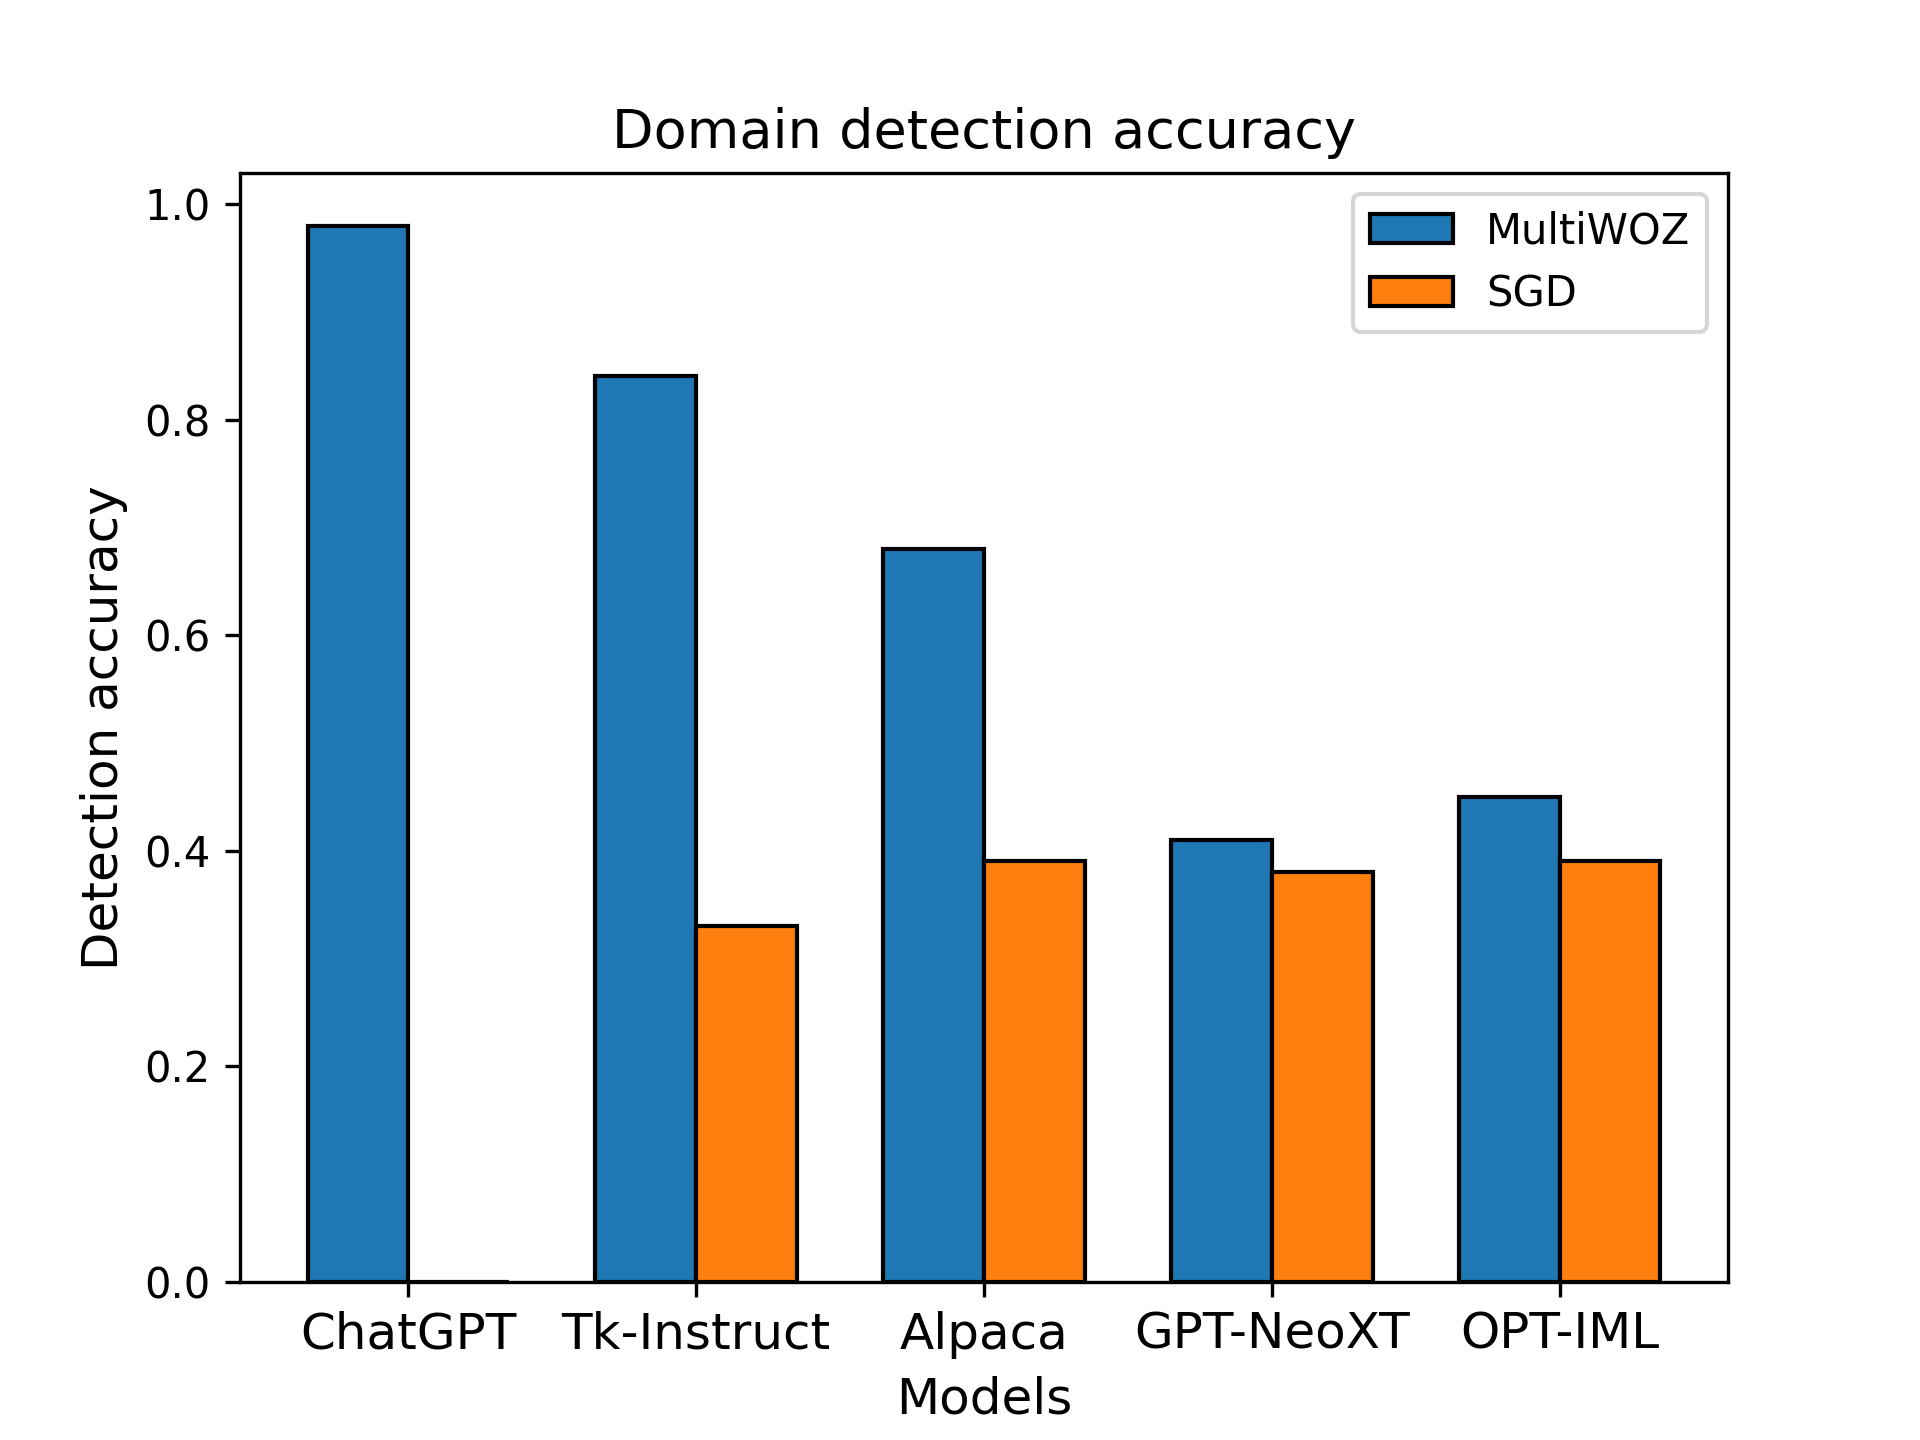
\includegraphics[width=0.49\textwidth]{images/domain-detections.png}
    \caption{Domain detection accuracy concerning different models for MultiWOZ 2.2 and SGD data, which consist of 7 and 18 domains, respectively.}
    \label{07:fig:domains}
\end{figure}


\section{Automatic Metrics Results}
\label{07:sec:results}

\subsection{Domain detection}
\label{subsec:domain}
We report the domain detection accuracy on MultiWOZ and SGD
in Figure~\ref{07:fig:domains}.
We observe that the domain detection accuracy varies quite a lot for most models.
This presumably affects the quality of the retrieved few-shot examples and the appropriateness of the subsequent prompts.
However, it is important to note that domain detection is turn-based, and arguably, some situations (e.g., providing an address, saying goodbye, etc.) are always handled similarly, even though they belong to different domains.
Therefore, not all the retrieved examples from misclassified domains necessarily contain unrelated contexts.
To explore this, we measure the performance of all models in case an oracle domain is given to them (Figure \ref{fig:oracle_domains}).
Interestingly, using the Oracle domain did not improve performance; it even worsened in some cases.
This suggests that the model-predicted domain is generally good enough, and additionally, providing the domain information does not contribute to the final system performance.
The negative influence on performance might be caused by forcing the system to filter out relevant examples.
The conversation snippets are domain-independent in multiple cases so that the retrieval might perform better even with a wrongly selected domain.
Forcing the ground truth domain examples in these cases can be potentially harmful.

%%%%%%%%%%%%%%%%%%%%%%%%%
% FIG 4 - oracle domain
%%%%%%%%%%%%%%%%%%%%%%%%%
\begin{figure}[h]
    \centering
    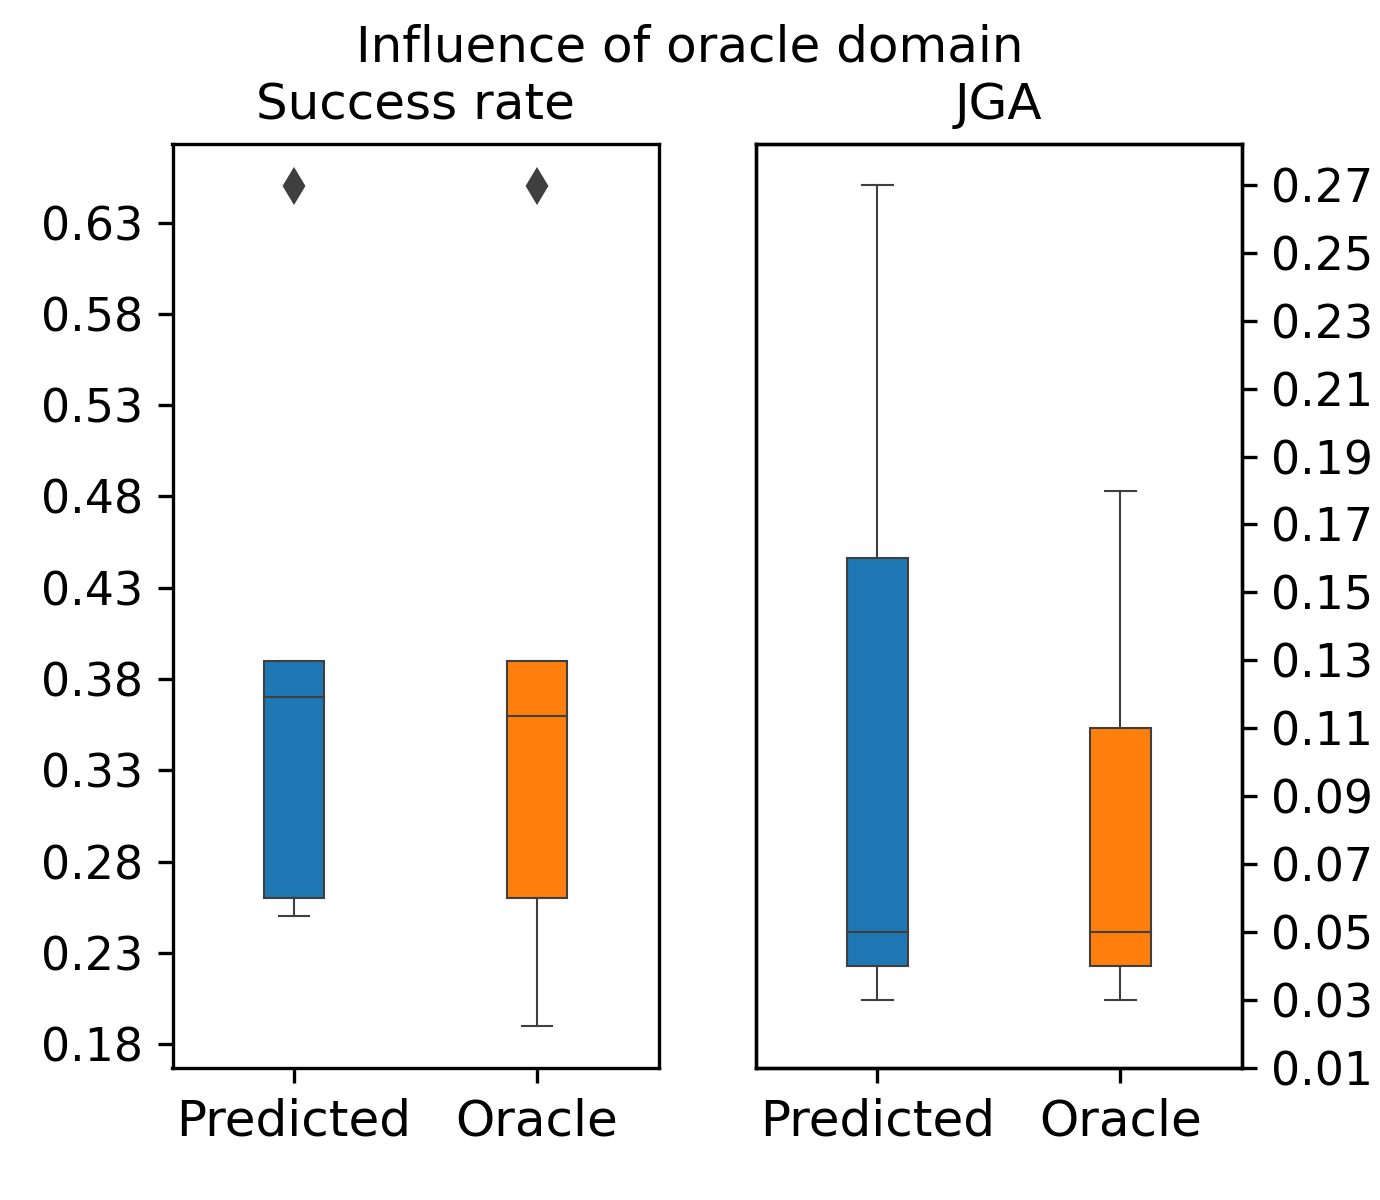
\includegraphics[width=0.49\textwidth]{images/oracle_domains.png}
    \caption{The influence of using oracle domain to retrieve examples. Interestingly, the oracle domain does not improve the performance, suggesting that the model-based detection is good enough for retrieval.}
    \label{fig:oracle_domains}
\end{figure}

\begin{table}[tp]
    \centering\small
    \begin{tabular}{l|c|c|ccc>{\hspace{-2mm}}c}
      \toprule
      model & few & oracle & \multicolumn{4}{c}{\textbf{MultiWOZ 2.2}} \\
      & shot & BS & BLEU & JGA & Slot-F1 & Success \\
      \midrule
      % Baselines
      Supervised SotA & \textcolor{red}{\xmark} & \textcolor{red}{\xmark} & 19.90$^\clubsuit$ & 0.60$^\diamondsuit$ & -- & 0.82$^\heartsuit$ \\
      % few-shot SotA & \textcolor{green}{\cmark} & \textcolor{red}{\xmark} & --& -- & -- & -- & BLEU & JGA & Slot-F1 & Success \\
      \midrule
      % ZS-GBS
      \rowcolor{tablegray}
      Alpaca-LoRA-7B-\emph{zs-gbs} & \textcolor{red}{\xmark} & \textcolor{red}{\xmark} & 1.61 & 0.06 & 0.07 & 0.04 \\
      \rowcolor{tablegray}
      Tk-Instruct-11B\emph{-zs-gbs} & \textcolor{red}{\xmark} & \textcolor{red}{\xmark} & 2.48 & 0.04 & 0.04 & 0.04 \\
      \rowcolor{tablegray}
      GPT-NeoXT-20B\emph{-zs-gbs} & \textcolor{red}{\xmark} & \textcolor{red}{\xmark} & 0.52 & 0.03 & 0.02 & 0.04 \\
      \rowcolor{tablegray}
      OPT-IML-30B\emph{-zs-gbs} & \textcolor{red}{\xmark} & \textcolor{red}{\xmark} & 0.56 & 0.02 & 0.04 & 0.03 \\
      \rowcolor{tablegray}
      ChatGPT\emph{-zs-gbs} & \textcolor{red}{\xmark} & \textcolor{red}{\xmark} & 4.17 & 0.13 & 0.40 & 0.31 \\ 

      % ZS-OBS
      Alpaca-LoRA-7B\emph{-zs-obs} & \textcolor{red}{\xmark} & \textcolor{green}{\cmark} & 1.73 & -- & -- & 0.08 \\
      Tk-Instruct-11B\emph{-zs-obs} & \textcolor{red}{\xmark} & \textcolor{green}{\cmark} & 2.66 & -- & -- & 0.18 \\
      GPT-NeoXT-20B\emph{-zs-obs} & \textcolor{red}{\xmark} & \textcolor{green}{\cmark} & 0.60 & -- & -- & 0.06 \\
      OPT-IML-30B\emph{-zs-obs} & \textcolor{red}{\xmark} & \textcolor{green}{\cmark} & 0.54 & -- & -- & 0.06 \\
      ChatGPT\emph{-zs-obs} & \textcolor{red}{\xmark} & \textcolor{green}{\cmark} & 3.76 & -- & -- & 0.47 \\ \midrule

      % FS- GBS
      \rowcolor{tablegray}
      Alpaca-LoRA-7B\emph{-fs-gbs} & \textcolor{green}{\cmark} & \textcolor{red}{\xmark} & 5.53 & 0.06 & 0.08 & 0.06\\
      \rowcolor{tablegray}
      Tk-Instruct-11B\emph{-fs-gbs} & \textcolor{green}{\cmark} & \textcolor{red}{\xmark} & 6.56 & 0.16 & 0.33 & 0.19 \\
      \rowcolor{tablegray}
      GPT-NeoXT-20B\emph{-fs-gbs} & \textcolor{green}{\cmark} & \textcolor{red}{\xmark} & 2.73 & 0.05 & 0.04 & 0.05 \\
      \rowcolor{tablegray}
      OPT-IML-30B\emph{-fs-gbs} & \textcolor{green}{\cmark} & \textcolor{red}{\xmark} & 4.40 & 0.03 & 0.03 & 0.04 \\
      \rowcolor{tablegray}
      ChatGPT\emph{-fs-gbs} & \textcolor{green}{\cmark} & \textcolor{red}{\xmark} & 6.77 & \textbf{0.27} & \textbf{0.51} & 0.44 \\

      % FS-OBS
      Alpaca-LoRA-7B\emph{-fs-obs} & \textcolor{green}{\cmark} & \textcolor{green}{\cmark} & 5.96 & -- & -- & 0.41 \\
      Tk-Instruct-11B\emph{-fs-obs} & \textcolor{green}{\cmark} & \textcolor{green}{\cmark} & \textbf{6.91} & -- & -- & 0.46 \\
      GPT-NeoXT-20B\emph{-fs-obs} & \textcolor{green}{\cmark} & \textcolor{green}{\cmark} & 2.92 & -- & -- & 0.28 \\
      OPT-IML-30B\emph{-fs-obs} & \textcolor{green}{\cmark} & \textcolor{green}{\cmark} & 5.40 & -- & -- & 0.28 \\
      ChatGPT\emph{-fs-obs} & \textcolor{green}{\cmark} & \textcolor{green}{\cmark} & 6.84 & -- & -- & \textbf{0.68} \\
     
    \bottomrule
  \end{tabular}
  \caption{
  Evaluation of the chosen LLMs concerning widely used TOD measures on the MultiWOZ dataset. For each model, we provide multiple variants. We use either zero-shot or few-shot prompts (\emph{-zs-} vs. \emph{-fs-}) and either generated or oracle belief state (\emph{-gbs} vs. \emph{-obs}).
  The few-shot variants use 10 examples per domain in the context storage, two selected for the prompts.  We also provide supervised state-of-the-art results to put the numbers in context: $^\clubsuit$\citet{sun2022mars}, $^\diamondsuit$\citet{huangrobustness}, $^\heartsuit$\citet{feng2023fantastic}. }
  \label{tab:res_overall_1}
\end{table}

\subsection{Response Generation}
BLEU scores are low overall, far below the supervised state-of-the-art.
Tk-Instruct and ChatGPT are the strongest here and perform roughly on par.
This behavior is likely because the models were not fine-tuned on the particular datasets, therefore they do not resemble the wording and phrasing used in this data.
Nevertheless, this observation does not necessary imply that the generated responses are incorrect.


\subsection{Belief State Tracking}
\label{subsec:dst}
The belief state tracking results overview is given in Tables \ref{tab:res_overall_1} and \ref{tab:res_overall_2} (\emph{JGA} and \emph{Slot-F1}).
A huge gap exists between the state-of-the-art supervised fine-tuned models' performance and the LLM results.
Also, our instruction-tuned LLMs fall short compared to \citet{hu-etal-2022-context}, who used few-shot in-context learning to formulate state tracking prompts for big LLMs such as OpenAI \texttt{davinci-codex}~\citep{chen2021evaluating} with 175B parameters and reported JGA 43.13\% with a comparable number of examples used for few-shot retrieval.
However, our models are generally an order of magnitude smaller, and we also use fewer examples in the prompt.
We hypothesize that the performance could be further improved by careful model-specific prompt customization and perhaps task re-formulation; nevertheless, this is not the goal of this work.
We intentionally focus on the universal framing of the task since we want to explore the general ability of the models to follow instructions.

When comparing the results among the models, ChatGPT outperforms the rest of the models by a large margin. 
Interestingly, the few-shot vs. zero-shot setting does not influence the results much for tracking, except for the GPT-NeoXT model.

\begin{table}[tp]
    \centering\small
    \begin{tabular}{l|c|c|ccc>{\hspace{-2mm}}c}
      \toprule
      model & few & oracle & \multicolumn{4}{c}{\textbf{Schema Guided Dialogues}} \\
      & shot & BS & BLEU & JGA & Slot-F1 & Success  \\
      \midrule
      % Baselines
      Supervised SotA & \textcolor{red}{\xmark} & \textcolor{red}{\xmark} & 29.90$^\ast$ & 0.30$^\dagger$ & 0.60$^\ast$ & --  \\
      % few-shot SotA & \textcolor{green}{\cmark} & \textcolor{red}{\xmark} & --& -- & -- & -- & BLEU & JGA & Slot-F1 & Success \\
      \midrule
      % ZS-GBS
      \rowcolor{tablegray}
      Alpaca-LoRA-7B\emph{-zs-gbs} & \textcolor{red}{\xmark} & \textcolor{red}{\xmark} & 2.79 & 0.02 & 0.01 & 0.11  \\
      \rowcolor{tablegray}
      Tk-Instruct-11B\emph{-zs-gbs} & \textcolor{red}{\xmark} & \textcolor{red}{\xmark} & 4.16 & 0.05 & 0.03 & 0.10  \\
      \rowcolor{tablegray}
      GPT-NeoXT-20B\emph{-zs-gbs} & \textcolor{red}{\xmark} & \textcolor{red}{\xmark} & 0.45 & 0.01 & 0.01 & 0.17 \\
      \rowcolor{tablegray}
      OPT-IML-30B\emph{-zs-gbs} & \textcolor{red}{\xmark} & \textcolor{red}{\xmark} & 1.63 & 0.01 & 0.01 & 0.17 \\
      \rowcolor{tablegray}
      % \emph{ChatGPT-zs-gbs} & \textcolor{red}{\xmark} & \textcolor{red}{\xmark} & -- & -- & -- & --  \\ 

      % ZS-OBS
      Alpaca-LoRA-7B\emph{-zs-obs} & \textcolor{red}{\xmark} & \textcolor{green}{\cmark} & 2.76 & -- & -- & 0.23  \\
      Tk-Instruct-11B\emph{-zs-obs} & \textcolor{red}{\xmark} & \textcolor{green}{\cmark} & 5.21 & -- & -- & 0.24  \\
      GPT-NeoXT-20B\emph{-zs-obs} & \textcolor{red}{\xmark} & \textcolor{green}{\cmark} & 0.83 & -- & -- & 0.22  \\
      OPT-IML-30B\emph{-zs-obs} & \textcolor{red}{\xmark} & \textcolor{green}{\cmark} & 1.94 & -- & -- & 0.22  \\
      % \emph{ChatGPT-zs-obs} & \textcolor{red}{\xmark} & \textcolor{green}{\cmark} & -- & -- & -- & --  \\ \midrule

      % FS- GBS
      \rowcolor{tablegray}
      Alpaca-LoRA-7B\emph{-fs-gbs} & \textcolor{green}{\cmark} & \textcolor{red}{\xmark} & 6.32 & 0.04 & 0.01 & 0.09 \\
      \rowcolor{tablegray}
      Tk-Instruct-11B\emph{-fs-gbs} & \textcolor{green}{\cmark} & \textcolor{red}{\xmark} & 6.66 & 0.06 & 0.05 & 0.10 \\
      \rowcolor{tablegray}
      GPT-NeoXT-20B\emph{-fs-gbs} & \textcolor{green}{\cmark} & \textcolor{red}{\xmark} & 1.62 & 0.04 & 0.02 & 0.09  \\
      \rowcolor{tablegray}
      OPT-IML-30B\emph{-fs-gbs} & \textcolor{green}{\cmark} & \textcolor{red}{\xmark} & 0.82 & \textbf{0.06} & \textbf{0.07} & 0.08  \\
      \rowcolor{tablegray}
      % \emph{ChatGPT-fs-gbs} & \textcolor{green}{\cmark} & \textcolor{red}{\xmark} & -- & -- & -- & --  \\

      % FS-OBS
      Alpaca-LoRA-7B\emph{-fs-obs} & \textcolor{green}{\cmark} & \textcolor{green}{\cmark} & 6.99 & -- & -- & \textbf{0.25} \\
      Tk-Instruct-11B\emph{-fs-obs} & \textcolor{green}{\cmark} & \textcolor{green}{\cmark} & \textbf{8.56} & -- & -- & \textbf{0.25} \\
      GPT-NeoXT-20B\emph{-fs-obs} & \textcolor{green}{\cmark} & \textcolor{green}{\cmark} & 1.97 & -- & -- & 0.24 \\
      OPT-IML-30B\emph{-fs-obs} & \textcolor{green}{\cmark} & \textcolor{green}{\cmark} & 0.56 & -- & -- & 0.22 \\
      % \emph{ChatGPT-fs-obs} & \textcolor{green}{\cmark} & \textcolor{green}{\cmark} & -- & -- & -- & -- \\

    \bottomrule
  \end{tabular}
  \caption{
  Evaluation of the chosen LLMs concerning widely used TOD measures on the SGD dataset. For each model, we provide multiple variants, as described in Table~\ref{tab:res_overall_1}.
  We also provide supervised state-of-the-art results to put the numbers in context: $^\ast$\citet{zhu2022convlab3}, $^\dagger$\citet{feng-etal-2021-sequence}. }
  \label{tab:res_overall_2}
\end{table}

\subsection{Dialogue-level performance}
\label{07:sec:dialogue-performance}
\begin{figure}[t]
    \centering
    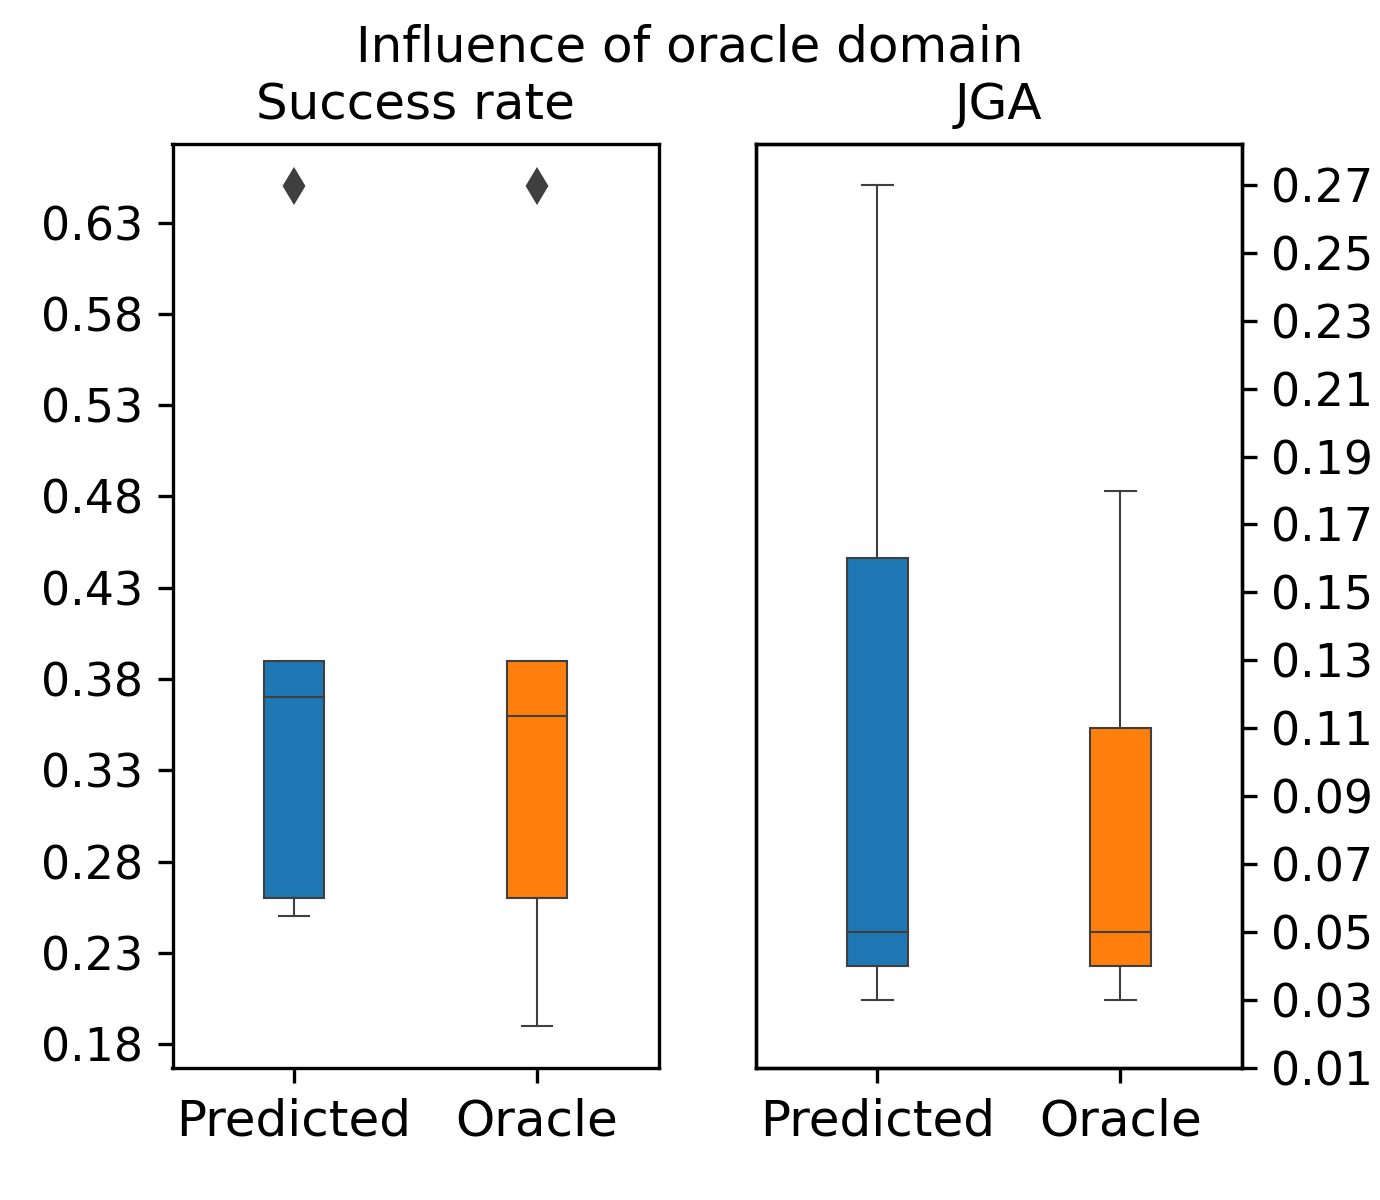
\includegraphics[width=0.49\textwidth]{images/oracle_domains.png}
    \caption{The influence of using oracle domain to retrieve examples. Interestingly, the oracle domain does not improve the performance, suggesting that the model-based detection is good enough for retrieval.}
    \label{07:fig:oracle_domains}
\end{figure}
%The ultimate measure to evaluate a task-oriented dialogue model is dialogue success.
Results for dialogue success are provided in Tables~\ref{tab:res_overall_1} and \ref{tab:res_overall_2}, and there is again a large gap between prompted LLMs and supervised custom models' performance.
ChatGPT seems to outperform other models, similarly to state tracking (cf.~Section~\ref{subsec:dst}).
In most cases, adding the retrieved few-shot examples helps.
The contribution of retrieved examples is more obvious when we supply the oracle belief state, which helps consistently for all the models.

We also explore the influence of the context storage size on the dialogue success rate.
The results are given in Figure~\ref{07:fig:shots}.
The biggest improvement can be achieved by supplying just a few examples instead of zero-shot prompting, but increasing the size of the example pool for retrieval does not yield further performance gains.
\begin{figure}[h]
    \centering
    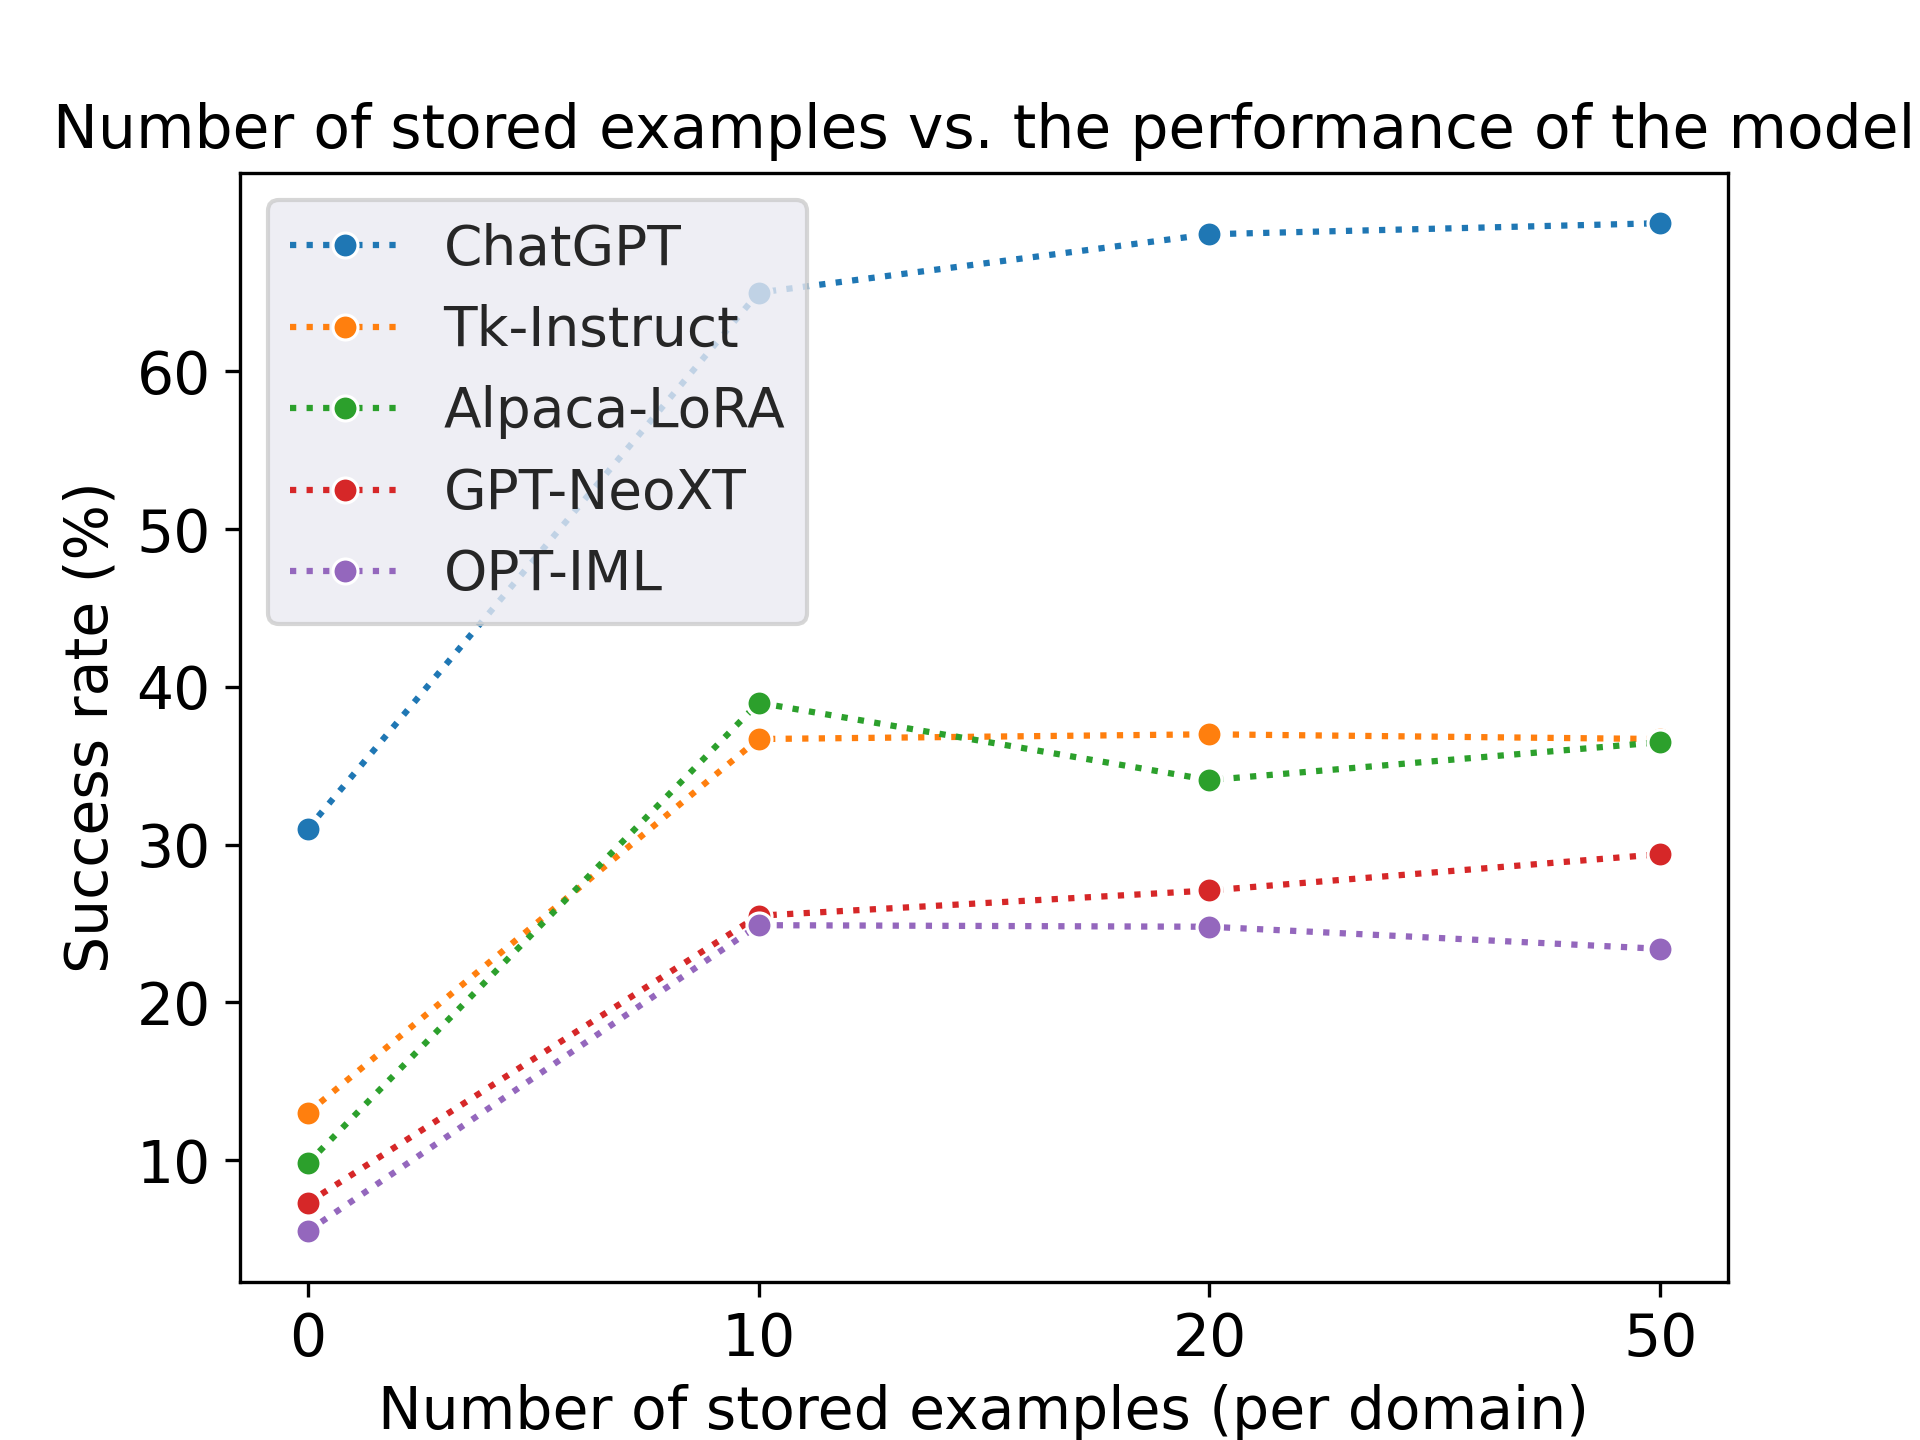
\includegraphics[width=0.9\textwidth]{images/shots.png}
    \caption{The influence of the number of examples per domain available for few-shot retrieval and response generation performance of the model in terms of the dialogue success on MultiWOZ 2.2 data with the oracle state supplied. Note that this does not represent the number of examples selected for the prompt, which is fixed to two.}
    \label{07:fig:shots}
\end{figure}

\subsection{Single-domain performance}
We evaluated the performance of the ChatGPT model when restricted to single-domain dialogues on MultiWOZ in Table~\ref{tab:single-domain}.
The average success rate is 0.76, which performs better then in case of the automatic metrics.
This outcome is expected as single-domain dialogues are typically shorter and easier to manage.
However, this observation can also give us interesting insights into the different performance values on the individual domains, which does not necessarily correlate with the number of slots or average dialogue length.
\begin{table}[tp]
    \centering
    \begin{tabular}{lccccc}
    \toprule
       domain  &  \textbf{Attraction} & \textbf{Taxi} & \textbf{Train} & \textbf{Hotel} & \textbf{Restaurant} \\ 
    \midrule
        success & 0.65 & 0.81 & 0.86 & 0.64 & 0.82 \\
    \bottomrule
    \end{tabular}
    \caption{Dialogue success of ChatGPT model when restricted to single domain dialogues in MultiWoz.}
    \label{tab:single-domain}
\end{table}
\section{Model Analysis}
\label{07:sec:analysis}

\subsection{Human Evaluation}
\label{07:sec:human}
We employed 6 annotators with a background in linguistics and NLP and let them interact with the two strongest models in terms of automatic metrics: ChatGPT and Tk-Instruct.
We present the results in Table~\ref{tab:human}.
We can see that in a real interaction with a human user and allowing for clarification or correction, the models perform better than the strict automatic evaluation.
Furthermore, the models are often successful in multiple sub-dialogues, even if a part of the dialogue fails.
The experiment also confirms the superior performance of ChatGPT on dialogue success and JGA.
Not surprisingly, given the above results, conversations with ChatGPT also required fewer clarification turns than with Tk-Instruct.

\begin{table}[tp]
    \centering
    \begin{tabular}{r|l}
    \toprule
         \textbf{Goal} & \texttt{You are looking for a train.}\\
         & \texttt{The train should depart from {\color{cyan!80!yellow!80!black!100 }Cambridge} and should leave} \\
         & \texttt{{\color{cyan!80!yellow!80!black!100 }after 9pm} on {\color{cyan!80!yellow!80!black!100 }thursday} and should go to {\color{cyan!80!yellow!80!black!100 }Stansted Airport}.} \\
         & \texttt{Once you find the train you want to} \\
         & \texttt{make a {\color{orange!50!yellow!90!black!100!}booking for 2 people}}\\
         & \texttt{Make sure you get the {\color{orange!50!yellow!90!black!100!}reference number}} \\
         \midrule
         \textbf{Customer} & \texttt{i need to find a train} \\
         & \texttt{from {\color{cyan!80!yellow!80!black!100 }cambridge} to {\color{cyan!80!yellow!80!black!100 }stansted airport}} \\
         \textbf{Assistant} & \texttt{what day will you be leaving?}\\
         \textbf{Customer} & \texttt{i need to leave on {\color{cyan!80!yellow!80!black!100 }thursday} {\color{cyan!80!yellow!80!black!100 }after 9pm.}}\\
         \textbf{Assistant} & \texttt{there is one on Thursday at {\color{orange!50!yellow!90!black!100!}21:08},}\\
         & \texttt{would you like me to book it for you?}\\
         \textbf{Customer} & \texttt{yes please, for 2 people} \\
         \textbf{Assistant} & \texttt{{\color{red!100!yellow!90!black!100!}Okay a honda will pick you up, the contact is [phone].}} \\
         & \texttt{Do you need anything else?} \\
         \textbf{Customer} & \texttt{i need to book the train for 2 people} \\
         \textbf{Assistant} & \texttt{{\color{red!100!yellow!90!black!100!}a honda will pick you up from cambridge }}\\
         & \texttt{{\color{red!100!yellow!90!black!100!}and the contact number is [phone].}}\\
         \textbf{Customer} & \texttt{i need a {\color{orange!50!yellow!90!black!100!}reference number} for the train} \\
         \textbf{Assistant} & \texttt{{\color{red!100!yellow!90!black!100!}TR8383 leaves Cambridge at 21:08 and}} \\
         & \texttt{{\color{red!100!yellow!90!black!100!}arrives at Stansted Airport at 21:36}.}\\
         \bottomrule
    \end{tabular}
    \caption{A sample evaluation conversation between human and LLM-based (ChatGPT) agent. The sample includes a textual goal description that instructs the user. The slot values are lexicalized in the assistant's responses. Here, the system {\color{red!100!yellow!90!black!100!} fails} to provide the requested information due to irrelevant examples (from taxi domain) in the retrieved context. The slot values are highlighted for both {\color{cyan!80!yellow!80!black!100 }informed} and {\color{orange!50!yellow!90!black!100!}requested} values.}
    \label{07:tab:human-2}
\end{table}
\subsection{Error Analysis}

To better understand the models' behavior, we manually inspect a random sample of ca.~20 dialogues for each model, chosen from cases where the automatic success metric was not satisfied. 
In general, we can split most erroneous behaviors into two distinct groups, which we call \emph{prompt-recoverable} and \emph{inherent}.

\paragraph{Prompt-recoverable errors} can be likely fixed by specific prompt engineering with some effort.
These kinds of errors happen with all of the tested models.
Examples of such errors are invalid structure of the generated dialogue state, copying slot values instead of using canonical values from the ontology, failure to delexicalize some of the values, etc.
Most of these errors can also be fixed in postprocessing -- for example, we can employ more robust parsers or fuzzy matching of slot values.

\paragraph{Inherent errors,} on the other hand, are likely not easily fixable by prompt modifications.
They are not distributed evenly across the tested models and seem to constitute a more challenging problem.

Perhaps the most important error, common to all the models, is hallucination, i.e., the model's output responses are not grounded in the context (such as offering entities that are not included in the database results). This happens in about 10-20\% of the inspected dialogues.
Some models (\emph{GPT-NeoXT, OPT-IML}) tend to generate more content than requested.
This happens in more than 50\% of their failed dialogues.
This sometimes means continuing the conversation for a few more turns (including hallucinating user turns), but the models also often generate unrelated text or even code snippets, see Table~\ref{07:tab:human-2}.
With \emph{Tk-Instruct}, we observed that in ca.~10\% cases, it copies the belief state from the example given in the prompt instead of generating a relevant one.
Another issue is that the models tend to repeat their previous responses as illustrated in Table~\ref{07:tab:human-1}.
\begin{table}[tp]
    \centering\small
    \begin{tabular}{l|r|r}
    \toprule
    & \textbf{ChatGPT} & \textbf{Tk-Instruct} \\
    \midrule
    dialogues & 25 & 25 \\
    subdialogues & 52 & 48 \\
    clarify / dial & 1.08 & 1.68 \\
    succesful subdialogues & 81\% & 71\% \\
    succesful dialogues & 76\% & 64\% \\
    correctly captured & 88\% & 66\% \\
    \bottomrule
    
    
    \end{tabular}
    \caption{Human evaluation results for ChatGPT and Tk-Instruct-11B models. We evaluate the conversation on the sub-dialogue level i.e. each domain in the dialogue is evaluated separately. }
    \label{tab:human}
\end{table}

\begin{table}[tp]
    \centering
    \begin{tabular}{r|l}
    \toprule
        \textbf{Goal} & \texttt{You are looking for information in Cambridge }\\
        & \texttt{You are looking for places to go in town.} \\
        & \texttt{The attraction should be a {\color{cyan!80!yellow!80!black!100 }swimming pool} and } \\
        & \texttt{should be {\color{cyan!80!yellow!80!black!100 }in the north.} }\\
        & \texttt{Make sure you get {\color{orange!50!yellow!90!black!100!}entrance fee.}}\\
        & \texttt{You are also looking for a train.}\\
        & \texttt{The train should go to {\color{cyan!80!yellow!80!black!100 }Cambridge} and {\color{cyan!80!yellow!80!black!100 }leave on Saturday.}}\\
        & \texttt{The train should depart from {\color{cyan!80!yellow!80!black!100 }London Liverpool Street}}\\
        & \texttt{and should {\color{cyan!80!yellow!80!black!100 }arrive by 20:00.}} \\
        & \texttt{Make sure you get {\color{orange!50!yellow!90!black!100!}travel time} and {\color{orange!50!yellow!90!black!100!}train ID}}.\\
        \midrule
        \textbf{Customer} & \texttt{I would like to {\color{cyan!80!yellow!80!black!100 }go swimming} in the {\color{cyan!80!yellow!80!black!100 }northern} cambridge}\\
        \textbf{Assistant} & \texttt{There is a swimming pool in the north.} \\
        & \texttt{Would you like more information on it?} \\
        \textbf{Customer} &\texttt{I would like to know the {\color{orange!50!yellow!90!black!100!}entrance fee}} \\
        \textbf{Assistant} & \texttt{The entrance fee for the pool is {\color{orange!50!yellow!90!black!100!}4 GBP}.} \\
        & \texttt{Can i help you with anything else?}\\
        \textbf{Customer} & \texttt{I am looking for a train from} \\
        & \texttt{{\color{cyan!80!yellow!80!black!100 }london liverpool street} to {\color{cyan!80!yellow!80!black!100 }cambridge}.} \\
        & \texttt{i would like to get there by {\color{cyan!80!yellow!80!black!100 }sunday 20:00}} \\
        \textbf{Assistant} & \texttt{you can take train which arrives at Cambridge at  {\color{orange!50!yellow!90!black!100!}19:07}} \\
        & \texttt{The price of the ticket is {\color{orange!50!yellow!90!black!100!}3 GBP}.} \\
        \textbf{Customer} & \texttt{what is the {\color{orange!50!yellow!90!black!100!}train id} and the {\color{orange!50!yellow!90!black!100!}travel time?}} \\
        \textbf{Assistant} & \texttt{{\color{orange!50!yellow!90!black!100!}TR2855} arrives at Cambridge at 19:07 on sunday.} \\
        \textbf{Customer} & \texttt{and the travel time} \\
        \textbf{Assistant} & \texttt{{\color{red!100!yellow!90!black!100!}TR2855 arrives at Cambridge at 19:07 on sunday.}} \\
        \textbf{Customer} & \texttt{how long will it take?} \\
        \textbf{Assistant} & \texttt{it will take you {\color{orange!50!yellow!90!black!100!}88 minutes} to get there. }\\
        \bottomrule
    \end{tabular}
    \caption{A sample evaluation conversation between human and LLM-based (ChatGPT) agent. The sample includes a textual goal description that instructs the user. The slot values are lexicalized in the assistant's responses. Although the systems {\color{red!100!yellow!90!black!100!}fails initially} and the customer needs to ask repeatedly about the duration of travel, it can get the desired information in the end. The slot values are highlighted for both {\color{cyan!80!yellow!80!black!100 }informed} and {\color{orange!50!yellow!90!black!100!}requested} values.}
    \label{07:tab:human-1}
\end{table}
%%%%%%%%%%%%%%%%%%%%%%%%%
% CONCLUSION
%%%%%%%%%%%%%%%%%%%%%%%%%
\section{Discussion}
We present an experimental evaluation of instruction-tuned LLMs applied to the established task of task-oriented dialogue modeling, with five LLMs evaluated on two datasets.
We find that current LLMs have difficulties concerning belief state tracking.
The LLM-based state trackers struggle even when provided with in-context few-shot examples.
Some problems arise because the LLM might not provide correctly formatted outputs.
These errors might be accounted for by restricting the decoding techniques and robust parsing mechanisms.
On the other hand, a non-trivial portion of errors come from hallucinated slot values that are not present in the conversation.
This behavior is harder to address successfully.

If provided with a correct belief state, the models can interact with the user well, provide useful information, and fulfill the user's needs.
While the performance does not match the supervised state of the art on the evaluated datasets, it is important to note that these models were not fine-tuned on in-domain data and work with just a domain description or a few examples (which improves performance). 
Moreover, few-shot examples improve the model performance and access to the oracle belief state.
Therefore, carefully picking representative examples and combining the LLM with an in-domain belief tracker can be a viable choice for a task-oriented dialogue pipeline.
Also, our evaluation experiments suggest that LLM-based systems are surprisingly good in human interaction, surpassing the results suggested by the corpus-based automatic evaluation metrics.

\paragraph{Limitations}
One of the drawbacks of our work is the reproducibility.
Closed models like ChatGPT are available only via API, and their behavior can change with time as out-of-date model are deprecated, making the experiments impossible to reproduce.
To address this, we include more models for the evaluation.
Another problem is the rapid development in this field of study.
New and stronger LLMs frequently appear, quickly making some of our results obsolete.
However, our experiments aim to put the LLM performance in context and show that despite their great capabilities, the approach of in-context learning is unlikely to solve the problem of task-oriented dialogues in the near future.

It would also be desirable to focus more on prompt engineering techniques since the LLMs are arguably sensitive to the choice of the right prompt, which is model-specific.

%%%%%%%%%%%%%%%%%%%%%%%%%%%%%%%%%%%%%%%%%%%%%%%%%%%%%%%%%%%%%%%%%%%%%%%%%%%%%
\chapter{Conclusion}
\label{chap:conclusion}
%%%%%%%%%%%%%%%%%%%%%%%%%%%%%%%%%%%%%%%%%%%%%%%%%%%%%%%%%%%%%%%%%%%%%%%%%%%%%
In this work, we discuss the problems of data annotation needed for task-oriented dialogue modeling.
We propose multiple approaches to tackle this issue.
In the following, we summarize our findings and formulate some of the conclusions we draw from the experiments.
Finally, we also discuss possible future research directions in this field.

\section{Unsupervised techniques for automatic data annotation}
Automatic data labeling procedures are desirable since they can save expensive resources by providing valuable insights into the gathered conversation data.
In Chapter~\ref{chap:data_analysis}, we propose a pipeline method for the unsupervised discovery of dialogue slot schema and automatic labeling.
The pipeline is generic because it can take an arbitrary set of input candidates, regardless of the candidate identification method.
We show that the method can successfully exploit the inputs and refine the initial candidate pool.
Moreover, we have shown that the outputs of our pipeline can be used as a noisy supervision for training task-oriented dialogue system models.

\section{Less supervision for end-to-end TOD models}
The ultimate goal is to be able to train task-oriented dialogue models solely from an unlabeled input corpus.
As an intermediate step toward this goal, we introduce a novel usage of latent variable models for TOD generation in Chapter~\ref{chap:modeling}.
In particular, we focus on latent system action modeling and providing the model with a means to communicate with external interfaces using only sparse annotations.
Modeling task-oriented dialogue this way is challenging, and achieving competitive performance with SoTA supervised models is hard.
However, our latent action models based on variational training show some promising properties and have the potential for interoperability.

Another direction is to use full supervision but minimize the amount of required training data.
We explore this path in Chapters~\ref{chap:lm-tod}~and~\ref{chap:llms}.
The power of pre-trained language models is great, and they can achieve good performance with only a fraction of the training set available to them.
Although they seem to struggle with the belief state tracking task, this can likely be fixed with fine-tuning techniques, and, according to our findings, the usage of large language models promises to bridge the gap between academic datasets and real-world use cases as they can handle various conversation behaviors very well. 

\section{Future research directions}
Unsupervised dialogue modeling will likely improve a lot in the future thanks to the tremendous progress in the field of large language models pre-training and applications.
LLMs can be used to obtain better representations and, together with contrastive learning objectives, achieve unseen performance in dialogue structure discovery and schema induction.
The modeling capabilities of the Transformer-based models will likely achieve significant improvements in human-machine interaction with little to no need to provide in-domain data examples.
Moreover, we might see a paradigm shift when instead of explicitly modeling the belief state, the models will communicate with APIs directly via in-line function calls.

%
% TEXT END
%

\renewcommand{\chapterheadstartvskip}{\vspace*{0mm}} % chapter spacing

\cleardoublepage{}
\bibliographystyle{csplainnat}
\addcontentsline{toc}{chapter}{Bibliography}
{\small \bibliography{references,anthology}}

\cleardoublepage{}
\addcontentsline{toc}{chapter}{List of Abbreviations}
\renewcommand*{\acronymname}{List of Abbreviations}
\printglossary[type=\acronymtype,style=index]

\addcontentsline{toc}{chapter}{List of Tables}
{\small \listoftables\par}

\addcontentsline{toc}{chapter}{List of Figures}
{\small \listoffigures\par}

\cleardoublepage{}
\addcontentsline{toc}{chapter}{List of Publications}
\chapter*{List of Publications}

\phantom{\nobibliography*{references}}
\noindent We first present list of publications in which the author of this thesis is the main author, followed with more publications to which the author contributed. The number of citations was computed using Google Scholar.

Total number of citations: 112 


\vfill

% -----------------------------------------------------------------------------
\noindent\bibentry{hudecek-etal-2021-discovering}
\begin{itemize}[noitemsep,topsep=0pt]

\item This work presents pipeline method for unsupervised slot discovery.
\item Citations: 20

\end{itemize}\vspace{.5\baselineskip}

% -----------------------------------------------------------------------------
\noindent\bibentry{hudecek-dusek-2023-large}
\begin{itemize}[noitemsep,topsep=0pt]

\item In this work we use large language models and in-context learning to model task-oriented dialogue.

\item Citations: 8
\end{itemize}\vspace{.5\baselineskip}


% -----------------------------------------------------------------------------
\noindent\bibentry{hudecek-dusek-2022-learning}
\begin{itemize}[noitemsep,topsep=0pt]

\item In this publication we introduce our dialogue model with variational training and discrete latent space.
\item Citations: 1

\end{itemize}\vspace{.5\baselineskip}

% -----------------------------------------------------------------------------
\noindent\bibentry{hudecek-etal-2022-unifying}
\begin{itemize}[noitemsep,topsep=0pt]

\item In this work we present novel dialogue corpus and related experiments.
\item Citations: 0

\end{itemize}\vspace{.5\baselineskip}


% -----------------------------------------------------------------------------
\noindent\bibentry{kulhanek-etal-2021-augpt}
\begin{itemize}[noitemsep,topsep=0pt]

\item This work presents the AuGPT model and related experiments. It also describes the DSTC 8 challenge participation.
\item Citations: 44

\end{itemize}\vspace{.5\baselineskip}

% -----------------------------------------------------------------------------
\noindent\bibentry{straka-etal-2018-sumeczech}
\begin{itemize}[noitemsep,topsep=0pt]

\item This publication describes a dataset that can be used for training of summarization models of news in Czech language and related experiments.
\item Citations: 22

\end{itemize}\vspace{.5\baselineskip}

% -----------------------------------------------------------------------------
\noindent\bibentry{platek2016recurrent}
\begin{itemize}[noitemsep,topsep=0pt]

\item In this publication we introduce an RNN-based model used to dialogue state tracking as a sequence modeling task.

\item Citations: 11

\end{itemize}\vspace{.5\baselineskip}

% -----------------------------------------------------------------------------
\noindent\bibentry{schaub-etal-2021-definition}
\begin{itemize}[noitemsep,topsep=0pt]

\item This work discusses the inconsistencies and problems found in dialogue corpora
\item Citations: 5

\end{itemize}\vspace{.5\baselineskip}

% -----------------------------------------------------------------------------
\noindent\bibentry{mukherjee2023polite}
\begin{itemize}[noitemsep,topsep=0pt]

\item In this work we explore the abilities of language models for text style transfer.
\item Citations: 1

\end{itemize}\vspace{.5\baselineskip}

% -----------------------------------------------------------------------------
\noindent\bibentry{platek2023three}
\begin{itemize}[noitemsep,topsep=0pt]

\item In this work we propose ways of evaluating dialogue qualities with large language models and describe our submission to the DSTC 11 challenge.
\item Citations: 0

\end{itemize}\vspace{.5\baselineskip}

\end{document}
